\chapter{Modular, Automorphic, \& Maass Forms}\label{ch:Modular_Maass_Automorphic_forms}
  Modular forms and Maass forms are special classes of functions on the upper-half space $\H$ of the complex plane. The former are holomorphic, have a transformation law with respect to a subgroup of $\PSL_{2}(\Z)$, and satisfy a growth condition. The latter are real-analytic, eigenfunctions with respect to the Laplace operator, invariant with respect to a subgroup of $\PSL_{2}(\Z)$, and satisfty a growth condition. We will introduce both of these forms in a general context as well as the more general automorphic forms. Before we introduce the forms themselves however, it is useful to discuss some of the theory about congruence subgroups of $\PSL_{2}(\Z)$ and modular curves. This small discussion will make the setup of modular, Maass, and automorphic forms more natural.
  \section{Congruence Subgroups \& Modular Curves}
    \subsection*{Congruence Subgroups}
      The \textbf{modular group}\index{modular group} is $\PSL_{2}(\Z) = \SL_{2}(\Z)/\{\pm I\}$. That is, the modular group is the set of matrices with integer entries and of determinant $1$ determined up to sign. The reason we are only interested in these matrices up to sign is because the modular group has a natural action on the upper-half space $\H$ and this action will be invariant under a change in sign. The first result usually proved about the modular group is that it is generated by two matrices:

      \begin{proposition}\label{prop:PSL_generator}
          \[
            \PSL_{2}(\Z) = \left\<\begin{pmatrix} 0 &-1 \\ 1 & 0 \end{pmatrix},\begin{pmatrix} 1 & 1 \\ 0 & 1 \end{pmatrix} \right\>.
          \]
      \end{proposition}
      \begin{proof}
        Set $S$ and $T$ to be the first and second generators respectively. Clearly they belong to $\PSL_{2}(\Z)$. Also, $S$ and $T^{n}$ for $n \in \Z$ acts on $\g = \begin{psmallmatrix} a & b \\ c & d \end{psmallmatrix} \in \PSL_{2}(\Z)$ by
        \[
          S\g = S\begin{pmatrix} a & b \\ c & d \end{pmatrix} = \begin{pmatrix} -c & -d \\ a & b \end{pmatrix} \quad \text{and} \quad T^{n}\g = T^{n}\begin{pmatrix} a & b \\ c & d \end{pmatrix} = \begin{pmatrix} a+nc & b+nd \\ c & d \end{pmatrix}.
        \]
        In particular, $S$ interchanges the upper left and lower left entries of $\g$ up to sign and $T^{n}$ adds an $n$ multiple of the lower left entry to the upper left entry. We have to show $\g \in \<S,T\>$ and we will acomplish this by showing that the inverse is in $\<S,T\>$. If $|c| = 0$ then $\g$ is the identity since $\det(\g) = 1$ so suppose $|c| \neq 0$. By Euclidean division we can write $a = qc+r$ for some $q \in \Z$ and $|r| < |c|$. Then
        \[
          T^{-q}\g = \begin{pmatrix} a-qc & b-qd \\ c & d \end{pmatrix} = \begin{pmatrix} r & b-qd \\ c & d \end{pmatrix}.
        \]
        Multiplying by $S$ yields
        \[
          ST^{-q}\g = S\begin{pmatrix} r & b-qd \\ c & d \end{pmatrix} = \begin{pmatrix} -c & -d \\ r & b-qd \end{pmatrix},
        \]
        and this matrix has the upper left entry at least as large as the lower left entry in norm. Actually the upper left entry is strictly larger since $|c| > |r|$ by Euclidean divison. Therefore if we repeatedly apply this procedure, it must terminate with the lower left entry vanishing. But then we have reached the identity matrix. Therefore we have show $\g$ has an inverse in $\<S,T\>$.
      \end{proof}

      We will also be intersted in special subgroups of the modular group defined by congruence conditions on their entries. For $N \ge 1$, set
      \[
        \G(N) = \left\{\begin{pmatrix} a & b \\ c & d \end{pmatrix} \in \PSL_{2}(\Z):\begin{pmatrix} a & b \\ c & d \end{pmatrix} \equiv \begin{pmatrix} 1 & 0 \\ 0 & 1 \end{pmatrix} \tmod{N}\right\}.
      \]
      Then $\G(N)$ is the kernel of the natural homomorphism $\PSL_{2}(\Z) \to \PSL_{2}(\Z/N\Z)$ so it is a normal subgroup with finite index. We call $\G(N)$ the \textbf{principal congruence subgroup}\index{principal congruence subgroup} of level $N$. For $\G \le \PSL_{2}(\Z)$, we say $\G$ is a \textbf{congruence subgroup}\index{congruence subgroup} if $\G(N) \le \G$ for some $N$ and the minimal such $N$ is called the \textbf{level}\index{level} of $\G$. Note that if $M \mid N$, then $\G(N) \le \G(M)$. Thus if $\G$ is a congruence subgroup of level $N$, then $\G(kN) \le \G$ for all $k \ge 1$. This implies that congruence subgroups are closed under intersection. Also, it turns out that the natural homomorphism $\PSL_{2}(\Z) \to \PSL_{2}(\Z/N\Z)$ is surjective:

      \begin{proposition}\label{prop:surjective_modulo_N_for_modular_group}
        The natural homomorphism $\PSL_{2}(\Z) \to \PSL_{2}(\Z/N\Z)$ is surjective.
      \end{proposition}
      \begin{proof}
        Suppose $\begin{psmallmatrix} \conj{a} & \conj{b} \\ \conj{c} & \conj{d} \end{psmallmatrix} \in \SL_{2}(\Z/N\Z)$. Then $\conj{a}\conj{d}-\conj{b}\conj{c} \equiv 1 \tmod{N}$ so by B\'ezout's identity (generalized to three integers) $(\conj{c},\conj{d},N) = 1$. We claim that there exists $s$ and $t$ such that $c = \conj{c}+sN$, $d = \conj{d}+tN$ with $(c,d) = 1$. Set $g = (\conj{c},\conj{d})$. Then $(g,N) = 1$ because $(\conj{c},\conj{d},N) = 1$. If $\conj{c} = 0$ then set $s = 0$ so $c = 0$ and choose $t$ such that $t \equiv 1 \tmod{p}$ for any prime $p \mid g$ and $t \equiv 0 \tmod{p}$ for any prime $p \nmid g$ and $p \mid \conj{d}$. Such a $t$ exists by the Chinese remainder theorem. Now if $p \mid (c,d)$, then either $p \mid g$ or $p \nmid g$. If $p \mid g$, then $p \mid d-\conj{d} = tN$ which is absurd since $t \equiv 1 \tmod{p}$ and $(t,N) = 1$. If $p \nmid g$, then $p \nmid d-\conj{d} = tN$ but this is also absurd since $t \equiv 0 \tmod{p}$. Therefore $(c,d) = 1$ as claimed. If $\conj{c} = 0$ then $\conj{d} \neq 0$, and we can proceed similarly. Since $(c,d) = 1$ there exists $a$ and $b$ such that $ad-bc = 1$. Then $\begin{psmallmatrix} a & b \\ c & d \end{psmallmatrix} \in \SL_{2}(\Z)$ and maps onto $\begin{psmallmatrix} \conj{a} & \conj{b} \\ \conj{c} & \conj{d} \end{psmallmatrix}$. This proves surjectivity.
      \end{proof}
      
        By \cref{prop:surjective_modulo_N_for_modular_group}, $[\PSL_{2}(Z):\G(N)] = |\PSL_{2}(\Z/N\Z)|$. Since $\G(N) \le \G$ and $\G(N)$ has finite index in $\PSL_{2}(\Z)$ so does $\G$. The subgroups
      \[
        \G_{1}(N) = \left\{\begin{pmatrix} a & b \\ c & d \end{pmatrix} \in \PSL_{2}(\Z):\begin{pmatrix} a & b \\ c & d \end{pmatrix} \equiv \begin{pmatrix} 1 & \ast \\ 0 & 1 \end{pmatrix} \tmod{N}\right\},
      \]
      and
      \[
        \G_{0}(N) = \left\{\begin{pmatrix} a & b \\ c & d \end{pmatrix} \in \PSL_{2}(\Z):\begin{pmatrix} a & b \\ c & d \end{pmatrix} \equiv \begin{pmatrix} \ast & \ast \\ 0 & \ast \end{pmatrix} \tmod{N}\right\},
      \]
      are particularly important and are congruence subgroups of level $N$. The latter subgroup is called the \textbf{Hecke congruence subgroup}\index{Hecke congruence subgroup} of level $N$. Note that $\G(N) \le \G_{1}(N) \le \G_{0}(N)$. If $\G$ is a general congruence subgroup, it is useful to find a generating set for $\G$ in order to reduce results about $\G$ to that of the generators. This is usually achieved by performing some sort of Euclidean division argument on the enrties of a matrix $\g \in \G$ using the supposed generating set to construct the inverse for $\g$. For example, this was the proof stragety employed in \cref{prop:PSL_generator}.
    \subsection*{Modular Curves}
      The modular group naturally acts on the Riemann sphere $\hat{\C}$ by M\"obius transformations (sometimes called fractional linear transformations). Explicitly, any $\g = \begin{psmallmatrix} a & b \\ c & d \end{psmallmatrix} \in \PSL_{2}(\Z)$ acts on $z \in \hat{\C}$ by
      \[
        \g z = \frac{az+b}{cz+d},
      \]
      where $\g \infty = \frac{a}{c}$ and $\g\left(-\frac{d}{c}\right) = \infty$. These are automorphisms of $\hat{\C}$. Now observe
      \[
        \Im(\g z) = \Im\left(\frac{az+b}{cz+d}\right) = \Im\left(\frac{az+b}{cz+d}\frac{c\conj{z}+d}{c\conj{z}+d}\right) = \Im\left(\frac{ac|z|^{2}+adz+bc\conj{z}+bd}{|cz+d|^{2}}\right) = \frac{\Im(z)}{|cz+d|^{2}},
      \]
      where the last equality follows because $\Im(\conj{z}) = -\Im(z)$ and $\det(\g) = ad-bc = 1$. Since $|cz+d|^{2} > 0$, this means that $\g$ preserves the sign of the imaginary part of $z$. So $\g$ preserves the upper half-space $\H$, the lower half-space $\conj{\H}$, and the extended real line $\hat{\R}$ respectively. In particular, $\g$ restricts to an automorphism on these subspaces. The first and last of these three is the most important for the theory of modular and Maass forms.

      We will also breifly discuss a property of the action of a congruence subgroup $\G$ on $\H$. A \textbf{Fushian group}\index{Fushian group} is any subgroup of $\PSL_{2}(\R)$ that acts properly discontinuously on $\H$. It turns out that the modular group is a Fushian group (see \cite{diamond2005first} for a proof):

      \begin{proposition}\label{prop:modular_group_is_Fushian}
        The modular group is a Fushian group.
      \end{proposition}

      Note that \cref{prop:modular_group_is_Fushian} immediately implies that any subgroup of the modular group is also Fushian. In particular, all congruence subgroups are Fushian. This lets us say a little more about the action of a congruence subgroup $\G$ on $\H$. Indeed, points in $\H$ are closed since $\H$ is Hausdorff. Now $\G$ is a Fushian group so it acts properly discontinuously on $\H$. These two facts together imply that the $\G$-orbit of any point in $\H$ is a discrete set. We will make use of this property later on, but for now we are ready to introduce modular curves.

      A \textbf{modular curve}\index{modular curve} is a quotient $\GH$ of the upper half-space $\H$ by a congruence subgroup $\G$. We give $\GH$ the quotient topology induced from $\H$ as a subset of the Riemann sphere $\hat{\C}$. This gives $\GH$ some nice topological properties (see \cite{diamond2005first} for a proof):
      
      \begin{proposition}\label{prop:modular_curves_topological_properties}
        For any congruence subgroup $\G$, the modular curve $\GH$ is connected and Hausdorff.
      \end{proposition}

      A \textbf{fundamental domain}\index{fundamental domain} for $\GH$ is a closed set $\mc{F}_{\G} \subseteq \H$ satisfing the following conditions:
      \begin{enumerate}[label=(\roman*)]
        \item Any point in $\H$ is $\G$-equivalent to a point in $\mc{F}_{\G}$.
        \item If two points in $\mc{F}_{\G}$ are $\G$-equivalent via a non-identity element, then they lie on the boundary of $\mc{F}_{\G}$.
        \item The interior of $\mc{F}_{\G}$ is a domain.
      \end{enumerate}
      In other words, $\mc{F}_{\G}$ is a complete set of representatives (possibly with overlap on the boundary) for $\GH$ that has a nice topological structure with respect to $\H$. Note that if $\mc{F}_{\G}$ is a fundamental domain then so is $\g\mc{F}_{\G}$ for any $\g \in \G$ and moreover $\H = \bigcup_{\g \in \G}\g\mc{F}_{\G}$. So the choice of $\mc{F}_{\G}$ is not unique. Intuitively, a fundamental domain is a geometric realization of $\GH$ which is often more fruitful than thinking of $\GH$ as an abstract set of equivalence classes. Moreover, it's suggestive that we can give $\GH$ a geometric structure and indeed we can (see \cite{diamond2005first} for more). Property (iii) is usually not included in the definition of a fundamental domain for many authors. The reason that we impose this additional property is because we will integrate over $\mc{F}_{\G}$ and so we want $\mc{F}_{\G}$ to genuinely represent a domain as a subset of $\H$. Our choice of measure will be the \textbf{hyperbolic measure}\index{hyperbolic measure} $d\mu = \frac{dx\,dy}{y^{2}}$ (see \cite{diamond2005first} for more). In any case, the prototypical fundamental domain is the following one for the modular group:

      \begin{proposition}\label{prop:fundamental_domain_modular_group}
        \[
          \mc{F} = \left\{z \in \H:|\Re(z)| \le \frac{1}{2}, |z| \ge 1\right\},
        \]
        is a fundamental domain for $\PSL_{2}(\Z)$.
      \end{proposition}
      \begin{proof}
        Set $\PSL_{2}(\Z) = \<S,T\>$ where $S$ and $T$ are as in \cref{prop:PSL_generator}. We first show any point in $\H$ is $\PSL_{2}(\Z)$-equivaent to a point in $\mc{F}$. Let $z = x+iy \in \H$. Then for any $\g = \begin{psmallmatrix} a & b \\ c & d \end{psmallmatrix} \in \PSL_{2}(\Z)$, we have
        \[
          \Im(\g z) = \frac{\Im(z)}{|cz+d|^{2}} = \frac{y}{(cx+d)^{2}+(cy)^{2}}.
        \]
        Since $\det(\g) = 1$ we cannot have $c = d = 0$. Then as $y \neq 0$, $|cz+d|^{2}$ is bounded away from zero and moreover there are finitely many pairs $(c,d)$ such that $|cz+d|^{2}$ is less than any given upper bound. Therefore there exists $\g_{0} \in \PSL_{2}(\Z)$ that minimizes $|cz+d|^{2}$ and hence maximizes $\Im(\g_{0}z)$. In particular,
        \[
          \Im(S\g_{0}z) = \frac{\Im(\g_{0}z)}{|\g_{0}z|^{2}} \le \Im(\g_{0}z).
        \]
        The inequality above implies $|\g_{0}z| \ge 1$. Since $\Im(T^{n}\g_{0}z) = \Im(\g_{0}z)$ for all $n \in \Z$, repeating the argument above with $T^{n}\g_{0}$ in place of $\g_{0}$, we see that $|T^{n}\g_{0}z| \ge 1$. But $T$ shifts the real part by $1$ so we can choose $n$ such that $|\Re(T^{n}\g_{0}z)| \le \frac{1}{2}$. Therefore $T^{n}\g_{0} \in \PSL_{2}(\Z)$ sends $z$ into $\mc{F}$ as desired. We will now show that if two points in $\mc{F}$ are $\PSL_{2}(\Z)$-equivalent via a non-identity element, then they lie on the boundary of $\mc{F}$. Since $\PSL_{2}(\Z)$ acts on $\H$ by automorphisms, by \cref{prop:PSL_generator} it suffices to show that $S$ and $T$ map $\mc{F}$ outside of $\mc{F}$ except for possibly the boundary. This is clear for $T$ since it maps the left boundary line $\{z:\Re(z) = -\frac{1}{2},|z| \ge 1\}$ to the right boundary line $\{z:\Re(z) = \frac{1}{2},|z| \ge 1\}$ and every other point of $\mc{F}$ is mapped to the right of this line. For $S$, note that it maps the semicircle $\{z:|z| = 1\}$ to itself (although not identically) and maps $\infty$ to zero. Since M\"obius transformations send circles to circles and lines to lines it follows that every other point of $\mc{F}$ is taken to a point enclosed by the semicircle $\{z:|z| = 1\}$. Lastly, the interior of $\mc{F}$ is a domain since it is open and path-connected. This finishes the proof.
      \end{proof}

      \begin{figure}[ht]
        \centering
        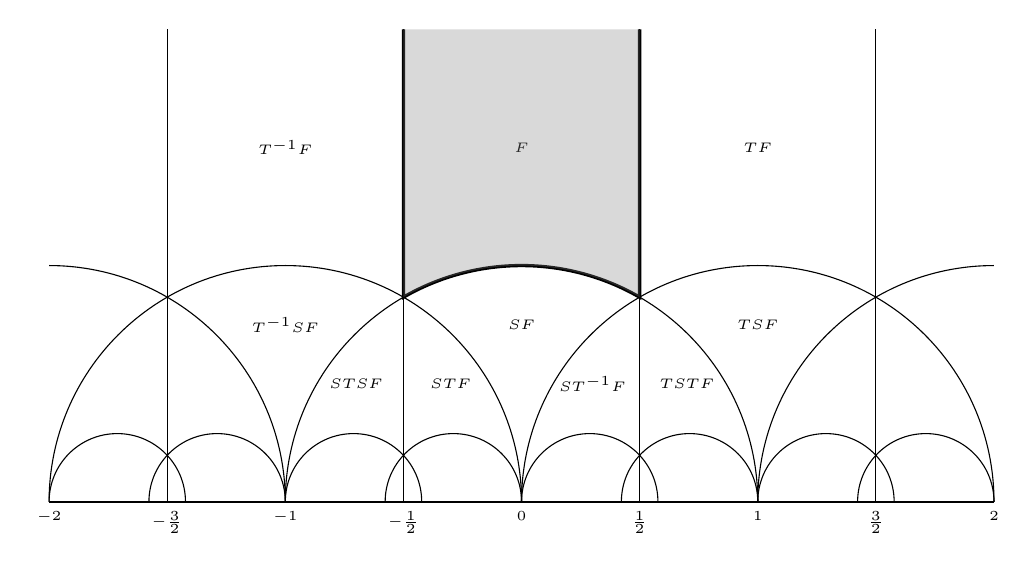
\begin{tikzpicture}[scale=3]
          \def\xmin{-2} \def\xmax{2}
          \def\ymin{0} \def\ymax{2}
          \draw[thick] (\xmin,0) -- (\xmax,0);

          \draw[very thick] (0.5,\ymax) -- (0.5,{sqrt(3)/2}) arc (60:120:1) -- (-0.5,\ymax);

          \node at (-0.5,0) [below] {\tiny{$-\frac{1}{2}$}};
          \node at (0.5,0) [below] {\tiny{$\frac{1}{2}$}};
          \node at (-1.5,0) [below] {\tiny{$-\frac{3}{2}$}};
          \node at (1.5,0) [below] {\tiny{$\frac{3}{2}$}};
          \node at (0,0) [below] {\tiny{$0$}};
          \node at (-1,0) [below] {\tiny{$-1$}};
          \node at (1,0) [below] {\tiny{$1$}};
          \node at (-2,0) [below] {\tiny{$-2$}};
          \node at (2,0) [below] {\tiny{$2$}};

          \draw[thin] (0.5,0) -- (0.5,\ymax);
          \draw[thin] (-0.5,0) -- (-0.5,\ymax);
          \draw[thin] (1.5,0) -- (1.5,\ymax);
          \draw[thin] (-1.5,0) -- (-1.5,\ymax);

          \draw (1,0) arc (0:180:1);
          \draw (-1,0) arc (0:90:1);
          \draw (2,1) arc (90:180:1);

          \draw (0,0) arc (0:180:1);
          \draw (2,0) arc (0:180:1);

          \draw (1,0) arc (0:180:{sqrt(3)/6});
          \draw ({sqrt(3)/3},0) arc (0:180:{sqrt(3)/6});

          \draw (2,0) arc (0:180:{sqrt(3)/6});
          \draw ({1+sqrt(3)/3},0) arc (0:180:{sqrt(3)/6});

          \draw (0,0) arc (0:180:{sqrt(3)/6});
          \draw ({(sqrt(3)/3)-1},0) arc (0:180:{sqrt(3)/6});

          \draw (-1,0) arc (0:180:{sqrt(3)/6});
          \draw ({(sqrt(3)/3)-2},0) arc (0:180:{sqrt(3)/6});

          \node at (0,1.5) {\tiny{$\mc{F}$}};
          \node at (-1,1.5) {\tiny{$T^{-1}\mc{F}$}};
          \node at (1,1.5) {\tiny{$T\mc{F}$}};
          \node at (0,0.75) {\tiny{$S\mc{F}$}};
          \node at (-1,0.75) {\tiny{$T^{-1}S\mc{F}$}};
          \node at (1,0.75) {\tiny{$TS\mc{F}$}};
          \node at (-0.7,0.5) {\tiny{$STS\mc{F}$}};
          \node at (-0.3,0.5) {\tiny{$ST\mc{F}$}};
          \node at (0.3,0.5) {\tiny{$ST^{-1}\mc{F}$}};
          \node at (0.7,0.5) {\tiny{$TST\mc{F}$}};

          \begin{scope}
            \path[clip] (0.5,\ymax) -- (0.5,{sqrt(3)/2}) arc (60:120:1) -- (-0.5,\ymax) -- cycle;
            \fill[gray,opacity=0.3] (-0.5,0) rectangle (0.5,\ymax);
          \end{scope}
        \end{tikzpicture}
        \caption{The standard fundamental domain for $\PSL_{2}(\Z)\backslash\H$.} \label{fig:fundamental_domain_modular_group}
      \end{figure}
      
      The shaded region in \cref{fig:fundamental_domain_modular_group} is the fundamental domain in \cref{prop:fundamental_domain_modular_group} and we call it the \textbf{standard fundamental domain}\index{standard fundamental domain}. \cref{fig:fundamental_domain_modular_group} also displays how this fundamental domain changes under the actions of the generators of $\PSL_{2}(\Z)$ as in \cref{prop:PSL_generator}. A fundamental domain for any other modular curve can be built from the standard fundamental domain as the following proposition shows (see \cite{kilford2015modular} for a proof):

      \begin{proposition}\label{prop:fundamental_domain_congruence_subgroup}
        Let $\G$ be any congruence subgroup. Then
        \[
          \mc{F}_{\G} = \bigcup_{\g \in \G\backslash\PSL_{2}(\Z)}\g\mc{F},
        \]
        is a fundamental domain for $\G\backslash\H$.
      \end{proposition}

      We might notice that $\mc{F}$ in \cref{fig:fundamental_domain_modular_group} is unbounded as it doesnt contain the point $\infty$. However, if we consider $\mc{F} \cup \{\infty\}$ then it would appear that this space is compact. The point $\infty$ is an example of a cusp and we now make this idea precise. Since any $\g \in \PSL_{2}(\Z)$ preserves $\hat{\R}$ and $\g$ has integer entries, $\g$ also preserves $\Q \cup \{\infty\}$. A \textbf{cusp}\index{cusp} of $\GH$ is an element of of $\G\backslash(\Q \cup \{\infty\})$. As $\G$ has finite index in the modular group, there can only be finitely many cusps and the number of cusps is at most the index of $\G$. In particular, the $\G$-orbit of $\infty$ is a cusp of $\GH$. We denote cusps by gothic characters $\mf{a},\mf{b},\mf{c},\ldots$ or by representatives of their equivalence classes. For example, we let $\infty$ denote the cusp $\G\infty$.

      \begin{remark}
        It turns out that the cusps can be represented as the points needed to make a fundmantal domain $\mc{F}_{\G}$ compact as a subset of $\hat{\C}$. To see this, suppose $\mf{a}$ is a limit point of $\mc{F}_{\G}$ that does not belong to $\mc{F}_{\G}$. Then $\mf{a} \in \hat{\R}$. In the case of the standard fundmantal domain $\mc{F}$, $\mf{a} = \infty$ which is a cusp. Otherwise, $\mc{F}_{\G}$ is a union of images of $\mc{F}$ by \cref{prop:fundamental_domain_congruence_subgroup} and since $\PSL_{2}(\Z)\infty = \Q \cup \{\infty\}$, we find that $\mf{a} \in \Q \cup \{\infty\}$.
      \end{remark}

      Let $\G_{\mf{a}} \le \G$ denote the stabilizer subgroup of the cusp $\mf{a}$. For the $\infty$ cusp, we can describe $\G_{\infty}$ explicitly. If $\g = \begin{psmallmatrix} a & b \\ c & d \end{psmallmatrix} \in \G$ stabilizes $\infty$, then necessarily $c = 0$ and since $\det(\g) = 1$ we must have $a = d = 1$. Therefore $\g = \begin{psmallmatrix} 1 & b \\ 0 & 1 \end{psmallmatrix}$ for some $b \in \Z$ and $\g$ acts on $\H$ by translation by $b$. Of course, not every translation is guaranteed to belong to $\G$. Letting $t$ be the smallest positive integer such that $\begin{psmallmatrix} 1 & t \\ 0 & 1 \end{psmallmatrix} \in \G$, we have $\G_{\infty} = \left\<\begin{psmallmatrix} 1 & t \\ 0 & 1 \end{psmallmatrix}\right\>$. In particular, $\G_{\infty}$ is an infinite cyclic group. We say that $\G$ is \textbf{reduced at infinity}\index{reduced at infinity} if $t = 1$ so that $\G_{\infty} = \left\<\begin{psmallmatrix} 1 & 1 \\ 0 & 1 \end{psmallmatrix}\right\>$. In particular, $\G_{0}(N)$ is reduced at infinity. In particular, $\G_{1}(N)$ and $\G_{0}(N)$ are reduced at infinity.
      
      \begin{remark}
        If $\G$ is of level $N$, then $N$ is the smallest positive integer such that $\G(N) \le \G$ so that $\begin{psmallmatrix} 1 & N \\ 0 & 1 \end{psmallmatrix}$ is the minimal translation guaranteed to belong to $\G$. However, there may be smaller translations so in general $t \le N$.
      \end{remark}
      
      Actually, for any cusp $\mf{a}$, $\G_{\mf{a}}$ is also an infinite cyclic group. To see this, if $\mf{a} = \frac{a}{c}$ with $(a,c) = 1$ is a cusp of $\GH$ not equivaent to $\infty$, then there exists an $\s_{\mf{a}} \in \PSL_{2}(\Z)$ such that $\s_{\mf{a}}\infty = \mf{a}$. Indeed, there exists integers $d$ and $b$ such that $ad-bc = 1$ by B\'ezout's identity and then $\s_{\mf{a}} = \begin{psmallmatrix} a & b \\ c & d \end{psmallmatrix}$ is such a matrix. It follows that $\G_{\mf{a}} = \s_{\mf{a}}\G_{\infty}\s_{\mf{a}}^{-1}$ and since $\G_{\infty}$ is infinite cyclic so is $\G_{\mf{a}}$. We call any matrix $\s_{\mf{a}} \in \PSL_{2}(\Z)$ such that $\s_{\mf{a}}\infty = \mf{a}$ a \textbf{scaling matrix}\index{scaling matrix} for the cusp $\mf{a}$. Note that $\s_{\mf{a}}$ is determined up to composition on the right by an element of $\G_{\infty}$ or composition on the left by an element of $\G_{\mf{a}}$. Scaling matrices are useful because they allow us to transfer information at the cusp $\mf{a}$ to the cusp at $\infty$. 

      Let $\mf{a}$ and $\mf{b}$ be cusps of $\GH$ with scaling matrices $\s_{\mf{a}}$ and $\s_{\mf{b}}$ respectively. When investigating modular forms, it will be useful to have a double coset decomposition for sets of the form $\s_{\mf{a}}^{-1}\G\s_{\mf{b}}$. This is referred to as the \textbf{Bruhat decomposition}\index{Bruhat decomposition} for $\G$:

      \begin{theorem}[Bruhat decomposition]
        Let $\G$ be any congruence subgroup and let $\mf{a}$ and $\mf{b}$ be cusps of $\GH$ with scaling matrices $\s_{\mf{a}}$ and $\s_{\mf{b}}$ respectively. Then we have the disjoint decomposition
        \[
          \s_{\mf{a}}^{-1}\G\s_{\mf{b}} = \d_{\mf{a},\mf{b}}\W_{\infty}\cup\bigcup_{\substack{c \ge 1 \\ d \tmod{c}}}\W_{d/c},
        \]
        where
        \[
        \W_{\infty} = \left\{\begin{pmatrix} \ast & b \\ 0 & \ast \end{pmatrix}:\begin{pmatrix} \ast & b \\ 0 & \ast \end{pmatrix} \in \s_{\mf{a}}^{-1}\G\s_{\mf{b}}\right\},
        \]
        and
        \[
          \W_{d/c} = \G_{\infty}\w_{d/c}\G_{\infty},
        \]
        for some $\w_{d/c} = \begin{psmallmatrix} \ast & \ast \\ c & d \end{psmallmatrix} \in \s_{\mf{a}}^{-1}\G\s_{\mf{b}}$ with $c \ge 1$.
      \end{theorem}
      \begin{proof}
        We first show that $\W_{\infty}$ is nonempty if and only if $\mf{a} = \mf{b}$. Indeed, if $\w_{\infty} \in \W_{\infty}$ then $\w_{\infty} = \s_{\mf{a}}^{-1}\g\s_{\mf{b}}$ for some $\g \in \G$. Then
        \[
          \g\mf{b} = \s_{\mf{a}}\w_{\infty}\s_{\mf{b}}^{-1}\mf{b} = \s_{\mf{a}}\w_{\infty}\infty = \s_{\mf{a}}\infty = \mf{a}.
        \]
        This shows that $\mf{a} = \mf{b}$. Conversely, suppose $\mf{a} = \mf{b}$. Then $\s_{\mf{a}}^{-1}\G\s_{\mf{b}}$ contains $\s_{\mf{a}}^{-1}\G_{\mf{a}}\s_{\mf{a}} = \G_{\infty}$ so that $\W_{\infty}$ is nonempty. So $\W_{\infty}$ is nonempty if and only if $\mf{a} = \mf{b}$. In this case, for any two elements $\w_{\infty} = \s_{\mf{a}}^{-1}\g\s_{\mf{a}}$ and $\w'_{\infty} = \s_{\mf{a}}^{-1}\g'\s_{\mf{a}}$ of $\W_{\infty}$, we have
        \[
          \g'\g^{-1}\mf{a} = \s_{\mf{a}}\w'_{\infty}w_{\infty}^{-1}\s_{\mf{a}}^{-1}\mf{a} = \s_{\mf{a}}\w'_{\infty}w_{\infty}^{-1}\infty = \s_{\mf{a}}\mf{a}.
        \]
        Hence $\g'\g^{-1} \in \G_{\mf{a}}$ which implies $\w'_{\infty}w_{\infty}^{-1} = \s_{\mf{a}}^{-1}\g'\g^{-1}\s_{\mf{a}} \in \s_{\mf{a}}^{-1}\G_{\mf{a}}\s_{\mf{a}} = \G_{\infty}$. Therefore
        \[
          \W_{\infty} = \G_{\infty}w_{\infty} = w_{\infty}\G_{\infty} = \G_{\infty}w_{\infty}\G_{\infty},
        \]
        where the latter two equalities hold because $w_{\infty}$ is a translation and translations commute. Every other element of $\s_{\mf{a}}^{-1}\g\s_{\mf{b}}$ belongs to one of the double cosets $\W_{d/c}$ with $c \ge 1$ (since we are working in $\PSL_{2}(\Z)$). The relation
        \[
          \begin{pmatrix} 1 & n \\ 0 & 1 \end{pmatrix}\begin{pmatrix} \ast & \ast \\ c & d \end{pmatrix}\begin{pmatrix} 1 & m \\ 0 & 1 \end{pmatrix} = \begin{pmatrix} \ast & \ast \\ c & d+cm \end{pmatrix},
        \]
        shows that $\W_{d/c}$ is determined uniquely by $c$ and $d \tmod{c}$. This completes the proof of the decomposition.
      \end{proof}

      As a first application, take $\mf{a} = \mf{b} = \infty$ and $\s_{\mf{a}} = \s_{\mf{b}} = I$. Then the Bruhat decomposition implies
      \[
        \GG \cong I\cup\bigcup_{\substack{c \ge 1 \\ d \tmod{c}}}\w_{d/c}\G_{\infty},
      \]
      since $\G_{\infty}\backslash\W_{\infty} = \G_{\infty}\backslash\G_{\infty} \cong I$. This shows that every element of $\GG$ corresponds to a unique $(c,d) \in \Z^{2}-\{\mathbf{0}\}$ with $c \ge 0$ and $d$ determined only modulo $c$ except when $c = 0$ in which case $d = 1$ (the pair $(1,0)$ corresponds to $I$). Of course, this correspondence might not be surjective since the double coset $\W_{d/c}$ may be empty if there is no $\w_{d/c} \in \s_{\mf{a}}^{-1}\G\s_{\mf{b}}$. For example, if $\G$ is of level $N$ then every $\g = \begin{psmallmatrix} a & b \\ c & d \end{psmallmatrix} \in \G$ satisfies $c \equiv 0 \tmod{N}$ so that
      \[
        \GG = I\cup\bigcup_{\substack{c \ge 1 \\ c \equiv 0 \tmod{N} \\ d \tmod{c}}}\w_{d/c}\G_{\infty}.
      \]
      However, we still may have other cosets which are empty since $\G$ being of level $N$ only guarantees that $c \equiv 0 \tmod{N}$. To figure out for what subset of pairs $(c,d)$ the correspondence is a bijection it suffices to determine the admissible $d$ not just the admissible $d \tmod {c}$. 
      
      \begin{remark}\label{rem:Bruhat_bijection}
        An exceptionally important case is for the Hecke congruence subgroups $\G_{0}(N)$ with $\mf{a} = \mf{b} = \infty$. Suppose $c \ge 1$ with $c \equiv 0 \tmod{N}$ and $d \tmod{c}$. By Bezout's identity there exists integers $a$ and $b$ with $ad-bc = 1$ so that $\g = \begin{psmallmatrix} a & b \\ c & d \end{psmallmatrix} \in \G_{0}(N)$ if and only if $(c,d) = 1$. So we must have $d \equiv 1 \tmod{c}$. Then the following correspondence implied by the Bruhat decomposition is a bijection:
        \[
          \GG = I\cup\bigcup_{\substack{c \ge 1, d \in \Z \\ c \equiv 0 \tmod{N} \\ (c,d) = 1}}\w_{d/c}\G_{\infty}.
        \]
      \end{remark}
  \section{The General Setup for Modular Forms}\label{sec:The_General_Setup_for_Modular_Forms}
    \subsection*{Modular Forms}
      Let $\G$ be a congruence subgroup of level $N$ and let $\chi$ be a Dirichlet character of conductor $q \mid N$. Define $\chi(\g) = \chi(d)$ if $\g = \begin{psmallmatrix} a & b \\ c & d \end{psmallmatrix} \in \G$. We say that a function $f:\H \to \C$ is a \textbf{modular form}\index{modular form} (or \textbf{holomorphic form}\index{holomorphic form}) of weight $k \in \Z_{\ge 1}$, level $N$, and \textbf{twisted}\index{twisted} by $\chi$, on $\GH$ if the following properties are satisfied:
      \begin{enumerate}[label=(\roman*)]
        \item $f$ is holomorphic on $\H$.
        \item $f(\g z) = \chi(\g)(cz+d)^{k}f(z)$ for all $\g = \begin{psmallmatrix} a & b \\ c & d \end{psmallmatrix} \in \G$.
        \item $f(\a z)$ remains bounded as $\Im(z) \to \infty$ for all $\a \in \PSL_{2}(\Z)$.
      \end{enumerate}
      Property (ii) is called the \textbf{modularity condition}\index{modularity condition} and we say $f$ is \textbf{modular}\index{modular}. If $\chi$ is the trivial character, we say $f$ is \textbf{untwisted}\index{untwisted}. We set $j(\g,z) = (cz+d)$ and call $j(\g,z)$ the \textbf{factor of modularity}\index{factor of modularity} of $f$. Property (iii) is called the \textbf{growth condition}\index{growth condition} and we say $f$ is \textbf{holomorphic at the cusps}\index{holomorphic at the cusps}. Also, we say $f$ is a \textbf{(holomorphic) cusp form}\index{(holomorphic) cusp form} if in addition,
      \begin{enumerate}[label=(\roman*)]
        \setcounter{enumi}{3}
        \item $f(\a z) \to 0$ as $\Im(z) \to \infty$ for all $\a \in \PSL_{2}(\Z)$.
      \end{enumerate}
      Modular forms also admit Fourier series. Let $\begin{psmallmatrix} 1 & t \\ 0 & 1 \end{psmallmatrix}$ be the smallest translation belonging to $\G$. By modularity,
      \[
        f(z+t) = f\left(\begin{pmatrix} 1 & t \\ 0 & 1 \end{pmatrix}z\right) = f(z),
      \]
      so that $f$ is $t$-periodic.

      \begin{remark}
        If $f$ is $t$-periodic, then we may think of $f$ as a function on $\G_{\infty}\backslash\H$. Taking representatives, $\G_{\infty}\backslash\H$ is a strip in $\H$ with bounded real part so that $f$ is a function on a domain with boudned real part.
      \end{remark}

      As $f$ is $t$-periodic it admits a Fourier series
      \[
        f(z) = \sum_{n \in \Z}a(n,y)e^{\frac{2\pi inx}{t}}.
      \]
      Actually, the Fourier coefficients $a(n,y)$ do not depend on $y$. To see this, since $f$ is holomorphic we know
      \[
        \frac{\del f}{\del\conj{z}} = \frac{1}{2}\left(\frac{\del f}{\del x}+i\frac{\del f}{\del y}\right) = 0.
      \]
      Substiuting in the Fourier series and equating coefficients we obtain the ODE
      \[
        2\pi na(n,y)+a'(n,y) = 0,
      \]
      where the $'$ indicates differentiation with respect to $y$. Solving this ODE (by separation of variables) we see that there exists an $a(n)$ such that
      \[
        a(n,y) = a(n)e^{-2\pi ny}.
      \]
      Using these constant coefficients instead, we say $f$ has a \textbf{Fourier series at the $\infty$ cusp}\index{Fourier series at the $\infty$ cusp}:
      \[
        f(z) = \sum_{n \in \Z}a(n)e^{\frac{2\pi inz}{t}}.
      \]
      Accordingly, we say $f$ is \textbf{holomorphic at infinity}\index{holomorphic at infinity} if
      \[
        \lim_{z \to \infty}\sum_{n \in \Z}a(n)e^{\frac{2\pi inz}{t}},
      \]
      exists and is finite. This is equivalent to $f(z)$ remaining bounded as $\Im(z) \to \infty$ and therefore the Fourier series is actually over all $n \ge 0$ (the negative terms do not exhibit decay as $\Im(z) \to \infty$ unless their Fourier coefficients vanish). Moreover, the limit above is $a(0)$ and $f$ will have exponential decay to $a(0)$ as $\Im(z) \to \infty$. Writing $z = x+iy$ and fixing any $y > 0$, $f$ restricts to a $t$-periodic smooth function on $\R$ that is integrable on $[0,t]$, as it is holomorphic, so we have
      \[
        a(n) = \int_{0}^{t}f_{\infty}(x+iy)e^{-\frac{2\pi inx}{t}}\,dx.
      \]
      For a general cusp $\mf{a}$ of $\GH$, let $\s_{\mf{a}}$ be a scaling matrix for $\mf{a}$. That is, $\s_{\mf{a}}\infty = \mf{a}$. Then $f(\s_{\mf{a}}z)$ is holomorphic at infinity precisely when $f(\s_{\mf{a}}z)$ remains bounded as $\Im(z) \to \infty$ which is to say that $f(z)$ remains bounded as $z \to \mf{a}$. This motivates the saying that $f$ is holomorphic at the cusps. More generally, $f$ has a \textbf{Fourier series at the $\mf{a}$ cusp}\index{Fourier series at the $\mf{a}$ cusp}:
      \[
        f(\s_{\mf{a}}z) = \sum_{n \ge 0}a_{\mf{a}}(n)e^{\frac{2\pi inz}{t}}.
      \]
      Also, the Fourier series above is independent of the scaling matrix because $f$ is $\G_{\infty}$-invariant and the set of scaling matrices is stable under multiplication from $\G_{\mf{a}}$ on the right. For ease of communication, if it is clear what cusp we are working at we will mention the Fourier series and its coefficients without regard to the cusp. The Fourier coefficients $a_{\mf{a}}(n)$ are then given by
      \[
        a_{\mf{a}}(n) = \int_{0}^{t}f(\s_{\mf{a}}(x+iy))e^{-\frac{2\pi inx}{t}}\,dx,
      \]
      for any fixed $y > 0$. Notice that $f$ is a cusp form precisely if $a_{\mf{a}}(0) = 0$ for every Fourier series of $f$ at every cusp $\mf{a}$. In particular, $f$ exhibits exponential decay to zero near the cusps. Since the Fourier series is independent of the scaling matrix used, we only need to check condition (iii) for a set of scaling matrices for the cusps since every element of $\PSL_{2}(\Z)$ is either a scaling matrix for a cusp or belongs to $\G_{\infty}$ depending on if it fixes $\infty$ or not.
    \subsection*{Twists \& Cocycles}
      Let $\G$ be a congruence subgroup of level $N$. Sometimes we will be interested in modular forms with nontrivial twists $\chi$ on $\GH$. To ensure that our modular forms are not identically zero, the weight $k$ depends on $\chi$. Indeed, if $f$ is a weight $k$ modular form on $\GH$, modularity implies
      \[
        f(z) = f\left(\begin{pmatrix} -1 & 0 \\ 0 & -1 \end{pmatrix}z\right) = \chi(-1)(-1)^{k}f(z),
      \]
      So $f$ is identically zero unless $\chi(-1) = (-1)^{k}$. In other words, if $\chi$ is odd then $k$ must be odd and if $\chi$ is even then $k$ must be even. If $\chi$ is the trival character, then the twist is actually trivial and so modular forms twisted by Dirichlet characters generalize untwisted modular forms.

      We will now discuss a very useful property that the factor of modularity satisfies. Let $\g,\g' \in \G$ and suppose $j(\g,z)$ is the factor of modularity of a modular form $f$ on $\GH$. Set $\g = \begin{psmallmatrix} a & b \\ c & d \end{psmallmatrix}$ and $\g' = \begin{psmallmatrix} a' & b' \\ c' & d' \end{psmallmatrix}$ so that $\g'\g = \begin{psmallmatrix} a'a+b'c & a'b+b'b \\ c'a+d'c & c'b+d'd \end{psmallmatrix}$. Then
      \begin{align*}
        j(\g',\g z)j(\g,z) &= \left(c'\frac{az+b}{cz+d}+d'\right)(cz+d) \\
        &= \left(c'\frac{az+b}{cz+d}+d'\right)(cz+d) \\
        &= (c'(az+b)+d'(cz+d)) \\
        &= (c'a+d'c)z+c'b+d'd) \\
        &= j(\g'\g,z).
      \end{align*}
      In short,
      \[
        j(\g'\g,z) =  j(\g',\g z)j(\g,z),
      \]
      and this is called the \textbf{cocycle condition}\index{cocycle condition} for $j(\g,z)$. The cocycle condition immediately implies that the factor of modularity is determined by any set of generators for $\G$. This is a very useful fact to remember because it is often easier to verify modularity on a generating set of a congruence subgroup.
  \section{The Theory of Modular Forms}\label{sec:The_Theory_of_Modular_Forms}
    In practice the primary congruence subgroups of interest are $\G_{1}(N)$ and $\G_{0}(N)$ because these are the congruence subgroups for which we have the theory of Hecke operators. These congruence subgroups are also reduced at infinity so all of the modular forms are $1$-periodic. Nevertheless, many of the following results will be stated for more general congruence subgroups so we will always be clear about what properties the implicit congruence subgroup satisfies. However, the level will always be denoted as $N$ unless otherwise specified. Moreover, it will be useful to consider modular forms as functions on $\G_{\infty}\backslash\H$ where the domain has bounded real part.
    \subsection*{Eisenstein \& Poincar\'e Series}
      Let $\G$ be a congruence subgroup of level $N$. We will introduce two important classes of modular forms on $\GH$ namely the Eisenstein series and the Poincar\'e series. For any weight $k \ge 4$ and Dirichlet character $\chi$ with conductor $q \mid N$, we define the \textbf{(holomorphic) Eisenstein series}\index{(holomorphic) Eisenstein series} $E_{k,\chi}$ of weight $k$ twised by $\chi$ on $\GH$ by
      \[
        E_{k,\chi}(z) = \sum_{\g \in \GG}\cchi(\g)j(\g,z)^{-k},
      \]

      \begin{remark}
        The reason why we restrict to $k \ge 4$ is because for $k = 0,2$ the Eisenstein series do not converge (see \cref{prop:general_lattice_sum_convergence_for_two_variables}).
      \end{remark}

      The Bruhat decomposition applied to $\GG$ implies
      \[
        E_{k,\chi}(z) \ll \sum_{(c,d) \in \Z^{2}-\{\mathbf{0}\}}\frac{1}{|cz+d|^{k}},
      \]
      and as $k \ge 4$, this latter series is locally absolutely uniformly convergent for $z \in \H$ by \cref{prop:general_lattice_sum_convergence_for_two_variables}. Hence $E_{k,\chi}(z)$ does too and so it is holomorphic on $\H$.

      \begin{remark}\label{rem:Eisenstein_series_on_modular_group}
        In the case of the modular group, the Bruhat decomposition implies that a set of representatives for the quotient $\GG$ is
      \[
        \left\{\begin{pmatrix} 1 & 0 \\ 0 & 1 \end{pmatrix}\right\} \cup \left\{\begin{pmatrix} \ast & \ast \\ c & d \end{pmatrix}:c \ge 1, d \in \Z, (c,d) = 1\right\}.
      \]
      Then $E_{k,\chi}$ is given by
        \[
          E_{k,\chi}(z) = 1+\sum_{\substack{c \ge 1, d \in \Z \\ (c,d) = 1}}\frac{\cchi(d)}{(cz+d)^{k}}.
        \]
      \end{remark}

      We now show that $E_{k,\chi}$ is modular. This is just a computation:
      \begin{align*}
        E_{k,\chi}(\g z) &= \sum_{\g' \in \GG}\cchi(\g')j(\g',\g z)^{-k} \\
        &= \sum_{\g' \in \GG}\cchi(\g')\left(\frac{j(\g'\g,z)}{j(\g,z)}\right)^{-k} && \text{cocycle condition} \\
        &= j(\g,z)\sum_{\g' \in \GG}\cchi(\g')j(\g'\g,z)^{-k} \\
        &= \chi(\g)j(\g,z)\sum_{\g' \in \GG}\cchi(\g')\cchi(\g)j(\g'\g,z)^{-k} \\
        &= \chi(\g)j(\g,z)\sum_{\g' \in \GG}\cchi(\g'\g)j(\g'\g,z)^{-k} \\
        &= \chi(\g)j(\g,z)\sum_{\g' \in \GG}\cchi(\g')j(\g',z)^{-k} && \text{$\g' \to \g'\g^{-1}$ bijection on $\G$} \\
        &= \chi(\g)j(\g,z)E_{k,\chi}(z),
      \end{align*}
      To verify holomorphy at the cusps, we will need a technical lemma:

      \begin{lemma}\label{lem:technical_Eisenstein_convergence_lemma}
        Let $a,b > 0$ be real numbers and consider the half-strip
        \[
          S_{a,b} = \{z \in \H:|\Re(z)| \le a, \Im(z) \ge b\}.
        \]
        Then there is a $\d \in (0,1)$ such that
        \[
          |nz+m| \ge \d|ni+m|,
        \]
        for all $n,m \in \Z$ and all $z \in S_{a,b}$.
      \end{lemma}
      \begin{proof}
        If $n = 0$ then any $\d$ is sufficient and this $\d$ is independent of $z$. If $n \neq 0$, then the desired inequality is equivalent to
        \[
          \left|\frac{z+\frac{m}{n}}{i+\frac{n}{m}}\right| \ge \d.
        \]
        So consider the function
        \[
          f(z,x) = \left|\frac{z+x}{i+x}\right|,
        \]
        for $z \in S_{a,b}$ and real $x$. It suffices to show $f(z,x) \ge \d$. As $z \in \H$, $z-x \neq 0$ so that $f(z,x)$ is continuous and $f(z,x) > 0$ for all $z$ and $x$. Now let $Y > b$ and consider the region
        \[
          S_{a,b}^{Y} = \{z \in \H:|\Re(z)| \le a, b \le \Im(z) \le Y\}.
        \]
        We claim that there exists a $Y$ such that if $\Im(z) > Y$ and $|x| > Y$ then $f(z,x)^{2} > \frac{1}{4}$. Indeed, we compute
        \[
          f(z,x)^{2} = \frac{(z+x)(\conj{z}+x)}{(i+x)(-i+x)} = \frac{|z|^{2}+2\Re(z)x+x^{2}}{1+x^{2}} \ge \frac{\Im(z)+x^{2}}{1+x^{2}},
        \]
        where in the inequality we have used that $|z|^{2} \ge \Im(z)$ and $\Re(z)$ is bounded. Now $\frac{x^{2}}{1+x^{2}} \to 1$ as $x \to \pm\infty$ so choosing $Y$ such that $|x| > Y$ implies $\frac{x^{2}}{1+x^{2}} \ge \frac{1}{4}$ yields
        \[
          \frac{\Im(z)+x^{2}}{1+x^{2}} \ge \frac{\Im(z)}{1+x^{2}}+\frac{x^{2}}{1+x^{2}} \ge \frac{\Im(z)}{1+x^{2}}+\frac{1}{4} > \frac{1}{4}.
        \]
        It follows that $f(z,x) > \frac{1}{2}$ outside of $S_{a,b}^{Y} \x [-Y,Y]$. But this latter region is compact and so $f(z,x)$ obtains a minimum $\d'$ on it. Then set $\d = \min\{\frac{1}{2},\d'\}$ and we are done.
      \end{proof}

      We can now show that $E_{k,\chi}$ is holomorphic at the cusps. Let $\s_{\mf{a}}$ be a scaling matrix for the cusp $\mf{a}$. Then
      \[
        E_{k,\chi}(\s_{\mf{a}}z) \ll \sum_{(c,d) \in \Z^{2}-\{\mathbf{0}\}}\frac{1}{|c\s_{\mf{a}}z+d|^{k}}.
      \]
      Now decompose this last sum as
      \[
        \sum_{(c,d) \in \Z^{2}-\{\mathbf{0}\}}\frac{1}{|c\s_{\mf{a}}z+d|^{k}} = \sum_{d \neq 0}\frac{1}{d^{k}}+\sum_{c \neq 0}\sum_{d \in \Z}\frac{1}{|c\s_{\mf{a}}z+d|^{k}} = 2\sum_{d \ge 1}\frac{1}{d^{k}}+2\sum_{c \ge 1}\sum_{d \in \Z}\frac{1}{|c\s_{\mf{a}}z+d|^{k}}.
      \]
      Since the first sum is bounded, it suffices to show that the double sum is bounded as $\Im(z) \to \infty$. To see this, let $\Im(z) \ge 1$ and $\d$ be as in \cref{lem:technical_Eisenstein_convergence_lemma}. Then for any integer $N \ge 1$ we can write
      \begin{align*}
        \sum_{c \ge 1}\sum_{d \in \Z}\frac{1}{|c\s_{\mf{a}}z+d|^{k}} &= \sum_{c+|d| \le N}\frac{1}{|c\s_{\mf{a}}z+d|^{k}}+\sum_{c+|d| > N}\frac{1}{|c\s_{\mf{a}}z+d|^{k}} \\
        &\le \sum_{c+|d| \le N}\frac{1}{|c\s_{\mf{a}}z+d|^{k}}+\sum_{c+|d| > N}\frac{1}{(\d|ci+d|)^{k}} \\
        &\le \sum_{c+|d| \le N}\frac{1}{|c\s_{\mf{a}}z+d|^{k}}+\frac{1}{\d^{k}}\sum_{c+|d| > N}\frac{1}{|ci+d|^{k}}.
      \end{align*}
      Since $\sum_{c \ge 1}\sum_{d \in \Z}\frac{1}{|ci+d|^{k}}$ converges by \cref{prop:general_lattice_sum_convergence_for_two_variables}, the second sum tends to zero as $N \to \infty$. As for the first sum, it is finite and each term tends to a finite value as $\Im(z) \to \infty$. Holomorphy at $\mf{a}$ follows. We collect all of this work as a theorem:

      \begin{theorem}
        Let $k \ge 4$ and $\chi$ be Dirichlet character with conductor $q \mid N$. The Eisenstein series
        \[
          E_{k,\chi}(z) = \sum_{\g \in \GG}\cchi(\g)j(\g,z)^{-k},
        \]
        is a weight $k$ modular form twisted by $\chi$ on $\GH$.
      \end{theorem}

      \begin{remark}
        The intuition behind the construction of the Eisenstein series $E_{k,\chi}$ is that $E_{k,\chi}$ is built by averaging the twist and factor of modularity over $\G$. Actually, this average happens over $\GG$ because $\G_{\infty}$ acts trivially since $j(\g,z) = 1$ if $\g \in \G_{\infty}$ as $\g = \begin{psmallmatrix} 1 & n \\ 0 & 1 \end{psmallmatrix}$ for some $n \in \Z$.
      \end{remark}

      Now we will discuss our second class of modular forms. For every $m \ge 1$, weight $k \ge 4$ and Dirichlet character $\chi$ with conductor $q \mid N$, we define the $m$-th \textbf{(holomorphic) Poincar\'e series}\index{(holomorphic) Poincar\'e series} $P_{m,k,\chi}$ of weight $k$ twisted by $\chi$ on $\GH$ by
      \[
        P_{m,k,\chi}(z) = \sum_{\g \in \GG}\cchi(\g)j(\g,z)^{-k}e^{2\pi im\g z}.
      \]
      We first need to verify that $P_{m,k,\chi}$ is actually well-defined. This amounts to checking $e^{2\pi im\g z}$ is independent of the representative $\g$. Indeed, if $\g'$ represents the same element as $\g$ in $\GG$, then they differ on the left by an element of $\eta_{\infty} \in \G_{\infty}$. So suppose $\g' = \eta_{\infty}\g$ with $\eta_{\infty} = \begin{psmallmatrix} 1 & n \\ 0 & 1 \end{psmallmatrix} \in \G_{\infty}$. Then
      \[
        e^{2\pi im\g' z} = e^{2\pi im\eta_{\infty}\g z} = e^{2\pi im(\g z+n)} = e^{2\pi im\g z}e^{2\pi imnz} = e^{2\pi im\g z},
      \]
      and hence $P_{m,k,\chi}$ is well-defined. To see that $P_{m,k,\chi}$ is holomorphic on $\H$, first note that $|e^{2\pi im\g z}| = e^{-2\pi m\Im(\g z)} < 1$ for all $\g \in \G$. Applying the Bruhat decomposition to $\GG$, we see that
      \[
        P_{m,k,\chi}(z) \ll \sum_{(c,d) \in \Z^{2}-\{\mathbf{0}\}}\frac{1}{|cz+d|^{k}}.
      \]
      As $k \ge 4$, this latter series is locally absolutely uniformly convergent for $z \in \H$ by \cref{prop:general_lattice_sum_convergence_for_two_variables}. Hence $P_{m,k,\chi}(z)$ does too and so it is holomorphic on $\H$.

      \begin{remark}
        In the case of the modular group, the Bruhat decomposition implies that a set of representatives for the quotient $\GG$ is
      \[
        \left\{\begin{pmatrix} 1 & 0 \\ 0 & 1 \end{pmatrix}\right\} \cup \left\{\begin{pmatrix} \ast & \ast \\ c & d \end{pmatrix}:c \ge 1, d \in \Z, (c,d) = 1\right\}.
      \]
      as in \cref{rem:Eisenstein_series_on_modular_group}. Then $P_{m,k,\chi}$ is given by
        \[
          P_{m,k,\chi}(z) = e^{2\pi imz}+\sum_{\substack{c \ge 1, d \in \Z \\ (c,d) = 1}}\cchi(d)\frac{e^{2\pi im\left(\frac{az+b}{cz+d}\right)}}{(cz+d)^{k}},
        \]
        where $a$ and $b$ are chosen such that $\det\left(\begin{psmallmatrix} a & b \\ c & d \end{psmallmatrix}\right) = 1$.
      \end{remark}

      We now show that $P_{m,k,\chi}$ is modular. This is just a computation:
      \begin{align*}
        P_{m,k,\chi}(\g z) &= \sum_{\g' \in \GG}\cchi(\g')j(\g',\g z)^{-k}e^{2\pi im\g'\g z} \\
        &= \sum_{\g' \in \GG}\cchi(\g')\left(\frac{j(\g'\g,z)}{j(\g,z)}\right)^{-k}e^{2\pi im\g'\g z} && \text{cocycle condition} \\
        &= j(\g,z)\sum_{\g' \in \GG}\cchi(\g')j(\g'\g,z)^{-k}e^{2\pi im\g'\g z} \\
        &= \chi(\g)j(\g,z)\sum_{\g' \in \GG}\cchi(\g')\cchi(\g)j(\g'\g,z)^{-k}e^{2\pi im\g'\g z} \\
        &= \chi(\g)j(\g,z)\sum_{\g' \in \GG}\cchi(\g'\g)j(\g'\g,z)^{-k}e^{2\pi im\g'\g z} \\
        &= \chi(\g)j(\g,z)\sum_{\g' \in \GG}\cchi(\g')j(\g',z)^{-k}e^{2\pi im\g'z} && \text{$\g' \to \g'\g^{-1}$ bijection on $\G$} \\
        &= \chi(\g)j(\g,z)P_{m,k,\chi}(z),
      \end{align*}
      Hence $P_{m,k,\chi}(z)$ is modular with factor of modularity $j(\g,z)$. To verify holomorphy at the cusps, let $\s_{\mf{a}}$ be a scaling matrix for the cusp $\mf{a}$. First note that $|e^{2\pi im\g\s_{\mf{a}}z}| = e^{-2\pi m\Im(\g\s_{\mf{a}}z)} < 1$. Then
      \[
        P_{m,k,\chi}(\s_{\mf{a}}z) \ll \sum_{(c,d) \in \Z^{2}-\{\mathbf{0}\}}\frac{1}{|c\s_{\mf{a}}z+d|^{k}},
      \]
      and now we can proceed in exactly the same way used to show that $E_{k,\chi}$ was holomorphic at the cusps. We collect all of this work as a theorem:

      \begin{theorem}
        Let $k \ge 4$ and $\chi$ be a Dirichlet character with conductor $q \mid N$. The Poincar\'e series
        \[
          P_{m,k,\chi}(z) = \sum_{\g \in \GG}j(\g,z)^{-1}e^{2\pi im\g z},
        \]
        is a weight $k$ modular form twisted by $\chi$ on $\GH$.
      \end{theorem}
    \subsection*{Spaces of Modular Forms}
      Let $\G$ be a congruence subgroup of level $N$. Clearly modular forms on $\GH$ of a fixed weight $k$ and twist $\chi$ are closed under addition and scalar multiplication and therefore form a vector space. Let $\mc{M}_{k}(\G,\chi)$ denote this space. Clearly cusp forms are closed under all of these operations so we have the corresponding subspaces $\mc{S}_{k}(\G,\chi)$. Moreover, if the character $\chi$ is the trivial character, or equivalently we are considering untwisted modular forms, we will surpress the dependence upon $\chi$. If $\G_{1}$ and $\G_{2}$ are two congruence subgroups such that $\G_{1} \le \G_{2}$, then we have the inclusion
      \[
        \mc{M}_{k}(\G_{2}) \subseteq \mc{M}_{k}(\G_{1}).
      \]
      So in general, the smaller the congruence subgroup the more modular forms there are. We will need a dimensionality result regarding the space of modular forms of a fixed weight. However, it will suffice to only require the result for untwised forms. The result is that $\mc{M}_{k}(\G)$ is never too large (see \cite{diamond2005first} for a proof):

      \begin{theorem}\label{thm:modular_forms_space_classification}
        Then $\mc{M}_{k}(\G)$ is finite dimensional.
      \end{theorem}

      Since $\mc{S}_{k}(\G)$ is a subspace of $\mc{M}_{k}(\G)$, \cref{thm:modular_forms_space_classification} implies that $\mc{S}_{k}(\G)$ is also finite dimensional. It turns out that $\mc{S}_{k}(\G)$ is naturally an inner product space. To see this, we define an operator on $\mc{S}_{k}(\G) \x \mc{M}_{k}(\G)$. Let $\mc{F}_{\G}$ be a fundamental domain for $\GH$ and set
      \[
        V_{\G} = \int_{\mc{F}_{\G}}\,d\mu.
      \]
      We call $V_{\G}$ the \textbf{volume}\index{volume} of $\GH$. Also, if $\mc{F}_{\G} = \mc{F}$ we write $V_{\G} = V$. In other words, $V$ is the volume of $\PSL_{2}(\Z)\backslash\H$. Since the integrand is $\G$-invariant, $V_{\G}$ is independent of the choice of fundamental domain. There is also a simple relation between $V_{\G}$ and the index of $\G$ in $\PSL_{2}(\Z)$:
      \begin{equation}\label{equ:Petersson_volume_relation}
        V_{\G} = [\PSL_{2}(\Z):\G]V,
      \end{equation}
      which follows immeditely from \cref{prop:fundamental_domain_congruence_subgroup}. Now for $f \in \mc{S}_{k}(\G)$ and $g \in \mc{M}_{k}(\G)$, define their \textbf{Petersson inner product}\index{Petersson inner product} by
      \[
        \<f,g\>_{\G} = \frac{1}{V_{\G}}\int_{\mc{F}_{\G}}f(z)\conj{g(z)}\Im(z)^{k}\,d\mu.
      \]
      If the congruence subgroup is clear from context we will supress the dependence upon $\G$. The integrand is also $\G$-invariant so that the integral independent of the choice of fundamental domain. The integral is also absolutely bounded by \cref{met:decay_compacta_integral} (since $f$ is a cusp form). These two facts together imply that the Petersson inner product is well-defined. Actually, we have the following proposition:

      \begin{proposition}\label{prop:Petersson_inner_product_hermitian}
        $\mc{S}_{k}(\G)$ is a Hilbert space with respect to Petersson inner product.
      \end{proposition}
      \begin{proof}
        Let $f,g \in \mc{S}_{k}(\G)$. Linearity of the integral immediately implies that the Petersson inner product is linear on $\mc{S}_{k}(\G)$. It is also positive definite since
        \[
          \<f,f\> = \frac{1}{V_{\G}}\int_{\mc{F}_{\G}}f(z)\conj{f(z)}\Im(z)^{k}\,d\mu = \frac{1}{V_{\G}}\int_{\mc{F}_{\G}}|f(z)|^{2}\Im(z)^{k}\,d\mu \ge 0,
        \]
        with equality if and only if $f$ is identically zero because $|f(z)|^{2}\Im(z)^{k} \ge 0$. To see that it is conjugate symetric, observe
        \begin{align*}
          \conj{\<g,f\>} &= \conj{\frac{1}{V_{\G}}\int_{\mc{F}_{\G}}g(z)\conj{f(z)}\Im(z)^{k}\,d\mu} \\
          &= \frac{1}{V_{\G}}\int_{\mc{F}_{\G}}\conj{g(z)\conj{f(z)}\Im(z)^{k}\,d\mu} \\
          &= \frac{1}{V_{\G}}\int_{\mc{F}_{\G}}\conj{g(z)}f(z)\Im(z)^{k}\,\conj{d\mu} \\
          &= \frac{1}{V_{\G}}\int_{\mc{F}_{\G}}\conj{g(z)}f(z)\Im(z)^{k}\,d\mu && \text{$d\mu = \frac{dx\,dy}{y^{2}}$} \\
          &= \frac{1}{V_{\G}}\int_{\mc{F}_{\G}}f(z)\conj{g(z)}\Im(z)^{k}\,d\mu \\
          &= \<f,g\>.
        \end{align*}
        So the Petersson inner product is a Hermitian inner product on $\mc{S}_{k}(\G)$. Since $\mc{S}_{k}(\G)$ is finite dimensional by \cref{thm:modular_forms_space_classification}, it follows immediately that $\mc{S}_{k}(\G)$ is a Hilbert space.
      \end{proof}

      \begin{remark}\label{rem:non-degeneracy_of_Petersson_inner_product}
        As a consequence of \cref{prop:Petersson_inner_product_hermitian}, the Petersson inner product is also non-degenerate on $\mc{S}_{k}(\G)$. Actually, for the exact same reasoning this holds on $\mc{S}_{k}(\G) \x \mc{M}_{k}(\G)$ wherever the Petersson inner product is defined.
      \end{remark}

      Now suppose $f \in \mc{S}_{k}(\G)$ with Fouier coefficients $a_{n}(f)$. Define linear functionals $\phi_{m,k}:\mc{S}_{k}(\G) \to \C$, for every $m \ge 1$, by
      \[
        \phi_{m,k}(f) = a_{m}(f).
      \]
      Since $\mc{S}_{k}(\G)$ is a finite dimensional Hilbert space, the Riesz representation theorem implies that there exists a unique $v_{m,k} \in \mc{S}_{k}(\G)$ such that
      \[
        \<f,v_{m,k}\> = \phi_{m,k}(f) = a_{m}(f).
      \]
      We would like to know what these cusp forms are. It turns out that $v_{m,k}$ will be the Poincar\'e series $P_{m,k,\chi}$ up to a normalization factor. To see this, we compute the inner product:
      \begin{align*}
        \<f,P_{m,k,\chi}\> &= \frac{1}{V_{\G}}\int_{\mc{F}_{\G}}f(z)\conj{P_{m,k,\chi}(z)}\Im(z)^{k}\,d\mu \\
        &= \frac{1}{V_{\G}}\int_{\mc{F}_{\G}}f(z)\sum_{\g \in \GG}\chi(\g)\conj{j(\g,z)^{-k}}e^{-2\pi im\conj{\g z}}\Im(z)^{k}\,d\mu \\
        &= \frac{1}{V_{\G}}\int_{\mc{F}_{\G}}f(z)\sum_{\g \in \GG}\frac{\chi(\g)j(\g,z)^{k}}{|j(\g,z)|^{2k}}e^{-2\pi im\conj{\g z}}\Im(z)^{k}\,d\mu \\
        &= \frac{1}{V_{\G}}\int_{\mc{F}_{\G}}f(\g z)\sum_{\g \in \GG}\frac{1}{|j(\g,z)^{k}|^{2k}}e^{-2\pi im\conj{\g z}}\Im(z)^{k}\,d\mu && \text{modularity} \\
        &= \frac{1}{V_{\G}}\int_{\mc{F}_{\G}}f(\g z)\sum_{\g \in \GG}e^{-2\pi im\conj{\g z}}\Im(\g z)^{k}\,d\mu && \text{$\Im(\g z)^{k} = \frac{\Im(z)^{k}}{|j(\g,z)|^{2k}}$.}
      \end{align*}
      We put this last integral into a different form. The idea is to rewrite the integral over the fundamental domain $\mc{F}_{\G}$ as an integral over the strip $\G_{\infty}\backslash\H$. First, observe
      \begin{align*}
        \frac{1}{V_{\G}}\int_{\mc{F}_{\G}}f(\g z)\sum_{\g \in \GG}e^{-2\pi im\conj{\g z}}\Im(\g z)^{k}\,d\mu &= \frac{1}{V_{\G}}\int_{\mc{F}_{\G}}\sum_{\g \in \GG}f(\g z)e^{-2\pi im\conj{\g z}}\Im(\g z)^{k}\,d\mu \\
        &= \frac{1}{V_{\G}}\sum_{\g \in \GG}\int_{\mc{F}_{\G}}f(\g z)e^{-2\pi im\conj{\g z}}\Im(\g z)^{k}\,d\mu && \text{DCT} \\
        &= \frac{1}{V_{\G}}\sum_{\g \in \GG}\int_{\g\mc{F}_{\G}}f(z)e^{-2\pi im\conj{z}}\Im(z)^{k}\,d\mu && \text{$z \to \g^{-1}z$.}
      \end{align*}
      Now $\H = \bigcup_{\g \in \G}\g\mc{F}_{\G}$ so that $\G_{\infty}\backslash\H = \bigcup_{\g \in \GG}\g\mc{F}_{\G}$. Therefore we can write
      \[
        \frac{1}{V_{\G}}\sum_{\g \in \GG}\int_{\g\mc{F}_{\G}}f(z)e^{-2\pi im\conj{z}}\Im(z)^{k}\,d\mu = \frac{1}{V_{\G}}\int_{\G_{\infty}\backslash\H}f(z)e^{-2\pi im\conj{z}}\Im(z)^{k}\,d\mu.
      \]
      The rest is a computation:
      \begin{align*}
        \frac{1}{V_{\G}}\sum_{\g \in \GG}\int_{\g\mc{F}_{\G}}f(z)e^{-2\pi im\conj{z}}\Im(z)^{k}\,d\mu &= \frac{1}{V_{\G}}\int_{\G_{\infty}\backslash\H}f(z)e^{-2\pi im\conj{z}}\Im(z)^{k}\,d\mu \\
        &= \frac{1}{V_{\G}}\int_{0}^{\infty}\int_{0}^{1}\sum_{n \ge 1}a_{n}(f)e^{2\pi i(n-m)x}e^{-2\pi(n+m)y}y^{k}\,\frac{dx\,dy}{y^{2}} \\
        &= \frac{1}{V_{\G}}\int_{0}^{\infty}\sum_{n \ge 1}\int_{0}^{1}a_{n}(f)e^{2\pi i(n-m)x}e^{-2\pi(n+m)y}y^{k}\,\frac{dx\,dy}{y^{2}} && \text{DCT} \\
        &= \frac{1}{V_{\G}}\int_{0}^{\infty}a_{m}(f)e^{-4\pi my}y^{k}\,\frac{dy}{y^{2}},
      \end{align*}
      where the last line follows because
      \begin{equation}\label{equ:Dirac_integral_representation}
        \int_{0}^{1}e^{2\pi i(n-m)x}\,dx = \d_{n-m,0},
      \end{equation}
      so that the inner integral cuts off all the terms except for the $n = m$ term. Then
      \begin{align*}
        \frac{1}{V_{\G}}\int_{0}^{\infty}a_{m}(f)e^{-4\pi my}y^{k}\,\frac{dy}{y^{2}} &= \frac{a_{m}(f)}{V_{\G}}\int_{0}^{\infty}e^{-4\pi my}y^{k-1}\,\frac{dy}{y} \\
        &= \frac{a_{m}(f)}{V_{\G}}\int_{0}^{\infty}e^{-4\pi my}y^{k-1}\,\frac{dy}{y} && \text{$y \to \frac{y}{4\pi m}$} \\
        &= \frac{a_{m}(f)}{V_{\G}(4\pi m)^{k-1}}\int_{0}^{\infty}e^{-y}y^{k-1}\,\frac{dy}{y} \\
        &= \frac{\G(k-1)}{V_{\G}(4\pi m)^{k-1}}a_{m}(f) && \text{definition of $\G(k-1)$.}
      \end{align*}
      In conclusion,
      \begin{equation}\label{equ:Petersson_inner_product_with_Poincare_series}
        \<f,P_{m,k,\chi}\> = \frac{\G(k-1)}{V_{\G}(4\pi m)^{k-1}}a_{m}(f).
      \end{equation}
      Now set $\wtilde{P_{m,k,\chi}} = \frac{V_{\G}(4\pi m)^{k-1}}{\G(k-1)}P_{m,k,\chi}$. For all cusp forms $f$ (actually any modular form where the Petersson inner product is defined),
      \[
        \<f,\wtilde{P_{m,k,\chi}}-v_{m,k}\> = 0.
      \]
      By \cref{rem:non-degeneracy_of_Petersson_inner_product} the Petersson inner product is non-degenerate so we conclude $v_{m,k} = \wtilde{P_{m,k,\chi}}$. In particular, this shows that the Poincar\'e series $P_{m,k,\chi}$ are cusp forms. We usually work with the Poincar\'e series $P_{m,k,\chi}$ instead of their normalized counterparts $\wtilde{P_{m,k,\chi}}$. In any case, with \cref{equ:Petersson_inner_product_with_Poincare_series} in hand we can prove the following result:

      \begin{theorem}
        The Poincar\'e series span $\mc{S}_{k}(\G)$.
      \end{theorem}
      \begin{proof}
        Let $f \in \mc{S}_{k}(\G)$ with Fourier coefficients $a_{n}(f)$. Since $\G(k-1) \neq 0$, \cref{equ:Petersson_inner_product_with_Poincare_series} implies $\<f,P_{m,k,\chi}\> = 0$ if and only if $a_{m}(f) = 0$. So $f$ is orthogonal to all the Poincar\'e series if and only if every Fourier coefficient $a_{m}(f)$ is zero. But this happens if and only if $f$ is identically zero.
      \end{proof}

      Let's return to the previous computation for a breif moment. The procedure of changing an integral over a fundamental domain $\mc{F}_{\G}$ into an integral over the strip $\G_{\infty}\backslash\H$, or vice versa, works in a more general setting and is called \textbf{unfolding the integral}\index{unfolding the integral} or \textbf{folding the integral}\index{folding the integral} respectively:

      \begin{method}[Unfolding/folding the integral]
        Suppose $\G$ is any congruence subgroup with fundamental domain $\mc{F}_{\G}$, and we are given an absolutely convergent integral of the form
        \[
          \int_{\mc{F}_{\G}}\sum_{\g \in \G'\backslash\G}f(\g z)\,d\mu,
        \]
        where $\G' \le \G$ is a subgroup ($f$ is not necessarily a modular form). Then the above integral can be written in the form
        \[
          \int_{\G'\backslash\H}f(z)\,d\mu.
        \]
        To do this use DCT to interchange the sum and integral and then make the change of variales $z \to \g^{-1}z$ to put the integral in the form
        \[
          \sum_{\g \in \G'\backslash\G}\int_{\g\F_{\G}}f(z)\,d\mu.
        \]
        Then observe $\H = \bigcup_{\g \in \G}\g\mc{F}_{\G}$ so that $\G'\backslash\H = \bigcup_{\g \in \G'\backslash\G}\g\mc{F}_{\G}$ and the desired result follows. Of course, this is an equality everywhere so we can also run the procedure in reverse.
      \end{method}
    \subsection*{Double Coset Operators}
      We are ready to introduce a class of general operators, depending upon double cosets, on any congruence subgroup $\G$ of level $N$. We will use these operators to define the diamond and Hecke operators. Recall that $j(\g,z) = (cz+d)$, where $\g = \begin{psmallmatrix} a & b \\ c & d \end{psmallmatrix} \in \G$, is the factor of modularity. Actually, $j(\g,z)$ makes sense for any $\g \in \GL_{2}^{+}(\Q)$ and we extend it accordingly. Let $\G_{1}$ and $\G_{2}$ be two congruence subgroups (not necessarily of the same level). For $\a \in \GL_{2}^{+}(\Q)$ consider the double coset
      \[
        \G_{1}\a\G_{2} = \{\g_{1}\a\g_{2}:\g_{1} \in \G_{1}, \g_{2} \in \G_{2}\}.
      \]
      Then $\G_{1}$ acts on the set $\G_{1}\a\G_{2}$ by left multiplication so that it decomposes into a disjoin union of orbit spaces. Thus
      \[
        \G_{1}\a\G_{2} = \bigcup_{\b \in \G_{1}\backslash\G_{1}\a\G_{2}}\G_{1}\b,
      \]
      where the sum is over the orbit representatives $\b$. However, in order for these operators to be well-defined it is necessary that the orbit decomposition above is a finite union. This is indeed the case and we will require two lemmas. The first is that congruence subgroups are preserved under conjugation by elements of $\GL_{2}^{+}(\Q)$ provided we restrict to those elements in $\PSL_{2}(\Z)$:

      \begin{lemma}\label{lem:coset_lemma_1}
        Let $\G$ be a congruence subgroup and let $\a \in \GL_{2}^{+}(\Q)$. Then $\a^{-1}\G\a \cap \PSL_{2}(\Z)$ is a congruence subgroup.
      \end{lemma}
      \begin{proof}
        Recall that if $\G$ is of level $M$, then $\G(kM) \le \G$ for every $k \ge 1$. Thus there is an integer $\wtilde{N}$ such that $\G(\wtilde{N}) \le \G$, $\wtilde{N}\a \in \GL_{2}^{+}(\Z)$, and $\wtilde{N}\a \in \GL_{2}^{+}(\Z)$. Now let $N = \wtilde{N}^{3}$ and notice that any $\g \in \G(N)$ is of the form
        \[
          \g = \begin{pmatrix} 1 & 0 \\ 0 & 1 \end{pmatrix}+N\begin{pmatrix} k_{1} & k_{2} \\ k_{3} & k_{4} \end{pmatrix},
        \]
        for $k_{1},\ldots,k_{4} \in \Z$. Therefore $\G(N) \subseteq I+N\Mat_{2}(\Z)$. Thus
        \[
          \a\G(N)\a^{-1} \le \a(I+N\Mat_{2}(\Z))\a^{-1} = I+\wtilde{N}\Mat_{2}(\Z).
        \]
        As every matrix in $\a\G(N)\a^{-1}$ has determinant $1$ and $\G(\wtilde{N}) \subseteq I+\wtilde{N}\Mat_{2}(\Z)$, it follows that $\a\G(N)\a^{-1} \le \G(\wtilde{N})$. As $\G(\wtilde{N}) \le \G$, we conclude
        \[
          \G(N) \le \a^{-1}\G\a,
        \]
        and intersecting with $\PSL_{2}(\Z)$ completes the proof.
      \end{proof}

      It is worthwhile to note that since congruence subgroups are closed under intersection, \cref{lem:coset_lemma_1} implies that $\a^{-1}\G_{1}\a \cap \G_{2}$ is a congruence subgroup for and two congruence subgroups $\G_{1}$ and $\G_{2}$ any any $\a \in \GL_{2}^{+}(\Q)$. Our second lemma gives a way to describe the orbit representatives for $\G_{1}\a\G_{2}$ in terms of coset representatives:

      \begin{lemma}\label{lem:coset_lemma_2}
        Let $\G_{1}$ and $\G_{2}$ be congruence subgroups and let let $\a \in \GL_{2}^{+}(\Q)$. Set $\G_{3} = \a^{-1}\G_{1}\a \cap \G_{2}$. Then left multiplication map
        \[
          \G_{2} \to \G_{1}\a\G_{2} \qquad \g_{2} \mapsto \a\g_{2},
        \]
        induces a bijection from the coset space $\G_{3}\backslash\G_{2}$ to the orbit space $\G_{1}\backslash\G_{1}\a\G_{2}$.
      \end{lemma}
      \begin{proof}
        We will show that the induced map is both surjective and injective. For surjectivity, the orbit representatives $\b$ of $\G_{1}\backslash\G_{1}\a\G_{2}$ are of the form $\b = \g_{1}\a\g_{2}$ for some $\g_{1} \in \G_{1}$ and $\g_{2} \in \G_{2}$. Since $\G_{1}$ is acting on $\G_{1}\a\G_{2}$ by left multiplication, $\b$ can be written as $\b = \a\g'_{2}$ for some $\g'_{2} \in \G_{2}$. This shows that the induced map is a surjection. To prove injectivity, let $\g_{2},\g'_{2} \in \G_{2}$ be such that the orbit space representatives $\a\g_{2}$ and $\a\g'_{2}$ are equivalent. That is,
        \[
          \G_{1}\a\g_{2} = \G_{1}\a\g'_{2}.
        \]
        This implies $\a\g_{2}(\g'_{2})^{-1} \in \G_{1}\a$ and so $\g_{2}(\g'_{2})^{-1} \in \a^{-1}\G_{1}\a$. But we also have $\g_{2}(\g'_{2})^{-1} \in \G_{2}$ and these two facts together imply $\g_{2}(\g'_{2})^{-1} \in \G_{3}$. Hence
        \[
          \G_{3}\g_{2} = \G_{3}\g'_{2},
        \]
        which shows that the induced map is also an injection.
      \end{proof}

      With these lemmas in hand, we can prove that the orbit decomposition of $\G_{1}\a\G_{2}$ is finite:

      \begin{proposition}\label{prop:double_congruence_subgroup_coset_decomposition_is_finite}
        Let $\a \in \GL_{2}^{+}(\Q)$. Then the orbit decomposition
        \[
          \G_{1}\a\G_{2} = \bigcup_{j}\G_{1}\b,
        \]
        with respect to the action of $\G_{1}$ by left multiplication, is a finite union.
      \end{proposition}
      \begin{proof}
        Let $\G_{3} = \a\G_{1}\a^{-1} \cap \G_{2}$. Then $\G_{3}$ acts on $\G_{2}$ by left multiplication. By \cref{lem:coset_lemma_2}, the number of orbits of $\G_{1}\backslash\G_{1}\a\G_{2}$ is the same as the number of cosets of $\G_{3}\backslash\G_{2}$ which is $[\G_{2}:\G_{3}]$. By \cref{lem:coset_lemma_1}, $\a^{-1}\G_{1}\a \cap \PSL_{2}(\Z)$ is a congruence subgroup and hence $[\PSL_{2}(\Z):\a^{-1}\G_{1}\a \cap \PSL_{2}(\Z)]$ is finite. As $\G_{2} = \PSL_{2}(\Z) \cap \G_{2}$ and $\G_{3} = \a^{-1}\G_{1}\a \cap \PSL_{2}(\Z) \cap \G_{2}$, it follows that $[\G_{2}:\G_{3}] \le [\PSL_{2}(\Z):\a^{-1}\G_{1}\a \cap \PSL_{2}(\Z)]$ completing the proof.
      \end{proof}

      In light of \cref{prop:double_congruence_subgroup_coset_decomposition_is_finite}, we will denote the orbit representatives by $\b_{j}$ to make it clear that there are finitely many. We can now introduce our operators. Fix some congruence subgroup $\G$ and consider $\mc{M}_{k}(\G)$. Then for $\a \in \GL_{2}^{+}(\Q)$, we define the operator $[\a]_{k}$ on $\mc{M}_{k}(\G)$ to be the linear operator given by
      \[
        (f[\a]_{k})(z) = \det(\a)^{k-1}j(\a,z)^{-k}f(\a z),
      \]
      for any $f \in \mc{M}_{k}(\G)$. Moreover, $[\a]_{k}$ is multiplicative. Indeed, if $\a,\a' \in \GL_{2}^{+}(\Q)$, then
      \begin{align*}
        ((f[\a']_{k})[\a]_{k})(z) &= \det(\a)^{k-1}j(\a,z)^{-k}(f[\a']_{k})(\a z) \\
        &= \det(\a')^{k-1}\det(\a)^{k-1}j(\a',\a z)^{-k}j(\a,z)^{-k}f(\a'\a z) \\
        &= \det(\a'\a)^{k-1}j(\a'\a,z)^{-k}f(\a'\a z) && \text{cocycle condition} \\
        &= (f[\a'\a]_{k})(z).
      \end{align*}
      Also, if $\g \in \G$ and we choose the representative with $\det(\g) = 1$, then the chain of equalities
      \[
        (f[\g]_{k})(z) = j(\g,z)^{-k}f(\g z) = f(z),
      \]
      is equivalent to the modularity of untwisted $f$ on $\GH$. Thus $f$ is an untwisted modular form on $\GH$ if and only if $f[\g]_{k} = f$ for all $\g \in \G$ where $\g$ is chosen to be the representative with positive determinant. Now let $\G_{1}$ and $\G_{2}$ be two congruence subgroups and let $\a \in \GL_{2}^{+}(\Q)$. We define the \textbf{double coset operator}\index{double coset operator} $[\G_{1}\a\G_{2}]_{k}$ on $\mc{M}_{k}(\G_{1})$ to be the linear operator given by
      \[
        (f[\G_{1}\a\G_{2}]_{k})(z) = \sum_{j}(f[\b_{j}]_{k})(z) = \sum_{j}\det(\b_{j})^{k-1}j(\b_{j},z)^{-k}f(\b_{j}z),
      \]
      for any $f \in \mc{M}_{k}(\G_{1})$. By \cref{prop:double_congruence_subgroup_coset_decomposition_is_finite} this sum is finite. It remains to check that $f[\G_{1}\a\G_{2}]_{k}$ is well-defined. Indeed, if $\b_{j}$ and $\b_{j}'$ belong to the same orbit, then $\b_{j}'\b_{j}^{-1} \in \G_{1}$. But then as $f \in \mc{M}_{k}(\G_{1})$, is it invariant under the $[\b_{j}'\b_{j}^{-1}]_{k}$ operator so that
      \[
        (f[\b_{j}]_{k})(z) = ((f[\b_{j}'\b_{j}^{-1}]_{k})[\b_{j}]_{k})(z) = (f[\b_{j}']_{k})(z),
      \]
      and therefore the $[\G_{1}\a\G_{2}]_{k}$ operator is well-defined. Actually, the map $[\G_{1}\a\G_{2}]_{k}$ preserves modular forms:

      \begin{proposition}\label{prop:double_coset_operator_preserves_subspaces_modular}
        For any two congruence subgroups $\G_{1}$ and $\G_{2}$, $[\G_{1}\a\G_{2}]_{k}$ maps $\mc{M}_{k}(\G_{1})$ into $\mc{M}_{k}(\G_{2})$. Moreover, $[\G_{1}\a\G_{2}]_{k}$ preserves the subspace of cusp forms.
      \end{proposition}
      \begin{proof}
        Suppose $f \in \mc{M}_{k}(\G_{1})$ and $\g \in \G_{2}$. Then
        \begin{align*}
          (f[\G_{1}\a\G_{2}]_{k})(\g z) &= \sum_{j}\det(\b_{j})^{k-1}j(\b_{j},\g z)^{-k}f(\b_{j}\g z) \\
          &= \sum_{j}\det(\b_{j}\g)^{k-1}j(\b_{j},\g z)^{-k}f(\b_{j}\g z) && \text{$\det(\g) = 1$} \\
          &= \sum_{j}\det(\b_{j}\g)^{k-1}\left(\frac{j(\g,z)}{j(\b_{j}\g,z)}\right)^{k}f(\b_{j}\g z) && \text{cocycle condition} \\
          &= j(\g,z)^{k}\sum_{j}\det(\b_{j}\g)^{k-1}j(\b_{j}\g,z)^{-k}f(\b_{j}\g z) \\
          &= j(\g,z)^{k}\sum_{j}\det(\b_{j})^{k-1}j(\b_{j},z)^{-k}f(\b_{j}z) && \text{$\b_{j} \to \b_{j}\g^{-1}$ bijection on $\G_{1}\a\G_{2}$} \\
          &= j(\g,z)^{k}\sum_{j}(f[\b_{j}]_{k})(z) \\
          &= j(\g,z)^{k}(f[\G_{1}\a\G_{2}]_{k})(z),
        \end{align*}
        So $f[\G_{1}\a\G_{2}]_{k}$ is modular. Holomorphy and the growth condition are immediate since the sum is finite by \cref{prop:double_congruence_subgroup_coset_decomposition_is_finite}. Therefore $f[\G_{1}\a\G_{2}]_{k} \in \mc{M}_{k}(\G_{2})$. To see that $[\G_{1}\a\G_{2}]_{k}$ preserves the subspace of cusp forms, let $\s_{\mf{a}}$ be a scaling matrix for the cusp $\mf{a}$ of $\G_{2}\backslash\H$ and let $f \in \mc{S}_{k}(\G_{1})$. For any orbit representative $\b_{j}$, $\b_{j}\s_{\mf{a}}$ takes $\infty$ to an element of $\Q \cup \{\infty\}$ since $\b_{j} \in \GL_{2}^{+}(\Q)$. In other words, $\b_{j}\s_{\mf{a}}\infty = \mf{b}$ for some cusp $\mf{b}$ of $\G_{1}\backslash\H$. Now choose an integer $r \ge 1$ such that $r\a \in \GL_{2}^{+}(\Z)$. As a consequence, there exist integers $n,m \ge 1$ such that $rj(\b_{j},\s_{\mf{a}}z) = |n\s_{\mf{a}}z+m|$. Then letting $\Im(z) > 1$ and $\d$ be as in \cref{lem:technical_Eisenstein_convergence_lemma}, we have
        \[
          j(\b_{j},\s_{\mf{a}}z) = \frac{|n\s_{\mf{a}}z+m|}{r} \ge \frac{\d|ni+m|}{r}.
        \]
        From this bound, we see that
        \[
          (f[\G_{1}\a\G_{2}]_{k})(\s_{\mf{a}}z) \ll \left(\frac{\d|ni+m|}{r}\right)^{-k}\sum_{j}\det(\b_{j})^{k-1}f(\b_{j}\s_{\mf{a}} z).
        \]
        As $f$ is a cusp form, it has exponential decay to zero near the cusps so that the sum on the right-hand side tends to zero as $\Im(z) \to \infty$. Then $f[\G_{1}\a\G_{2}]_{k}$ is a cusp form too.
      \end{proof}

      The double coset operators are the most basic types of operators on modular forms. They are the building blocks needed to define the more important diamond and Hecke operators.
    \subsection*{Diamond \& Hecke Operators}
      The diamond and Hecke operators are special linear operators that are used to construct a linear theory of modular forms. They will also help us understand the Fourier coefficients. Throughout this discussion, we will obtain corresponding results for modular forms twisted by Dirichlet characters. We will discuss the diamond operator first. To define them, we need to consider both the congruence subgroups $\G_{1}(N)$ and $\G_{0}(N)$. Recall that $\G_{1}(N) \le \G_{0}(N)$ and consider the map
      \[
        \G_{0}(N) \to (\Z/N\Z)^{\ast} \qquad \begin{pmatrix} a & b \\ c & d\end{pmatrix} \to d \tmod{N},
      \]
      ($d$ is invertible modulo $N$ since $c \equiv 0 \tmod{N}$ and $ad-bc = 1$). This is a surjective homomorphism and its kernel is exaclty $\G_{1}(N)$ so that $\G_{1}(N)$ is a normal subgroup of $\G_{0}(N)$ and $\G_{0}(N)/\G_{1}(N) \cong (\Z/N\Z)^{\ast}$. Letting $\a = \begin{psmallmatrix} \ast & \ast \\ \ast & d \end{psmallmatrix} \in \G_{0}(N)$ and $f \in \mc{M}_{k}(\G_{1})$, consider $\left(f\left[\G_{1}(N)\a\G_{1}(N)\right]_{k}\right)(z)$. This is only dependent upon the lower-right entry $d$ of $\a$ taken modulo $N$. To see this, since $\G_{1}(N)$ is normal in $\G_{0}(N)$, $\G_{1}(N)\a = \a\G_{1}(N)$ so that $\G_{1}(N)\a\G_{1}(N) = \a\G_{1}(N)$ and hence there is only one representative for the orbit decomposition. Therefore
      \[
        \left(f\left[\G_{1}(N)\a\G_{1}(N)\right]_{k}\right)(z) = \sum_{j}(f[\b]_{k})(z) = (f[\a]_{k})(z).
      \]
      This induces an action of $\G_{0}(N)$ on $\mc{M}_{k}(\G_{1})$ and since $\G_{1}(N)$ acts trivially, this is really an action of $\G_{0}(N)/\G_{1}(N) \cong (\Z/N\Z)^{\ast}$. In other words, we have an induced action that depends only upon the lower-right entry $d$ of $\a$ taken modulo $N$. So for any $d$ modulo $N$, we define the \textbf{diamond operator}\index{diamond operator} $\<d\>:\mc{M}_{k}(\G_{1}(N)) \to \mc{M}_{k}(\G_{1}(N))$ to be the linear operator given by
      \[
        (\<d\>f)(z) = (f[\a]_{k})(z),
      \]
      for any $\a = \begin{psmallmatrix} \ast & \ast \\ \ast & d \end{psmallmatrix} \in \G_{0}(N)$. Our discussion above has already shown that the diamond operators $\<d\>$ are well-defined. Also, since the operator $[\a]_{k}$ is multiplicative and
      \[
        \begin{pmatrix} \ast & \ast \\ 0 & d \end{pmatrix}\begin{pmatrix} \ast & \ast \\ 0 & e \end{pmatrix} \equiv \begin{pmatrix} \ast & \ast \\ 0 & de \end{pmatrix} \tmod{N},
      \]
      the diamond operators are multiplicative. One reason the diamond operators are useful is that they decompose $\mc{M}_{k}(\G_{1}(N))$ into eigenspaces. For any Dirichlet character $\chi$ modulo $N$, we let
      \[
        \mc{M}_{k}(N,\chi) = \{f \in \mc{M}_{k}(\G_{1}(N)):\<d\>f = \chi(d)f \text{ for all } d \in (\Z/N\Z)^{\ast}\},
      \]
      be the $\chi$-eigenspace. Also let $\mc{S}_{k}(N,\chi)$ be the corresponding subspace of cusp forms. Then $\mc{M}_{k}(\G_{1}(N))$ admits a decomposition into these eigenspaces:

      \begin{proposition}\label{thm:diamond_operator_decomposition_modular}
        We have the direct sum decomposition
        \[
          \mc{M}_{k}(\G_{1}(N)) = \bigop_{\chi \tmod{N}}\mc{M}_{k}(N,\chi).
        \]
        Moreover, this direct sum decomposition respects the subspace of cusp forms.
      \end{proposition}
      \begin{proof}
        We have a representation of $\G_{0}(N)/\G_{1}(N) \cong (\Z/N\Z)^{\ast}$ over $\mc{M}_{k}(\G_{1}(N))$ given by the diamond operators. Explicitely,
        \[
          \Phi:(\Z/N\Z)^{\ast} \x \mc{M}_{k}(\G_{1}(N)) \to \mc{M}_{k}(\G_{1}(N)) \qquad (d,f) \to \<d\>f.
        \]
        But any representation of a finite abelian group over $\C$ is completely reducible with repect to the characters of the group and every irreducible subrepresentation is $1$-dimensional (see \cref{append:Representation_Theory}). Since the characters of $(\Z/N\Z)^{\ast}$ are given by Dirichlet characters, the result follows.
      \end{proof}
      
      If $\g = \begin{psmallmatrix} \ast & \ast \\ \ast & d \end{psmallmatrix} \in \G_{0}(N)$ and we choose the representative with positive determinant, then $\chi(\g) = \chi(d)$ and the chain of equalities
      \[
        (\<d\>f)(z) = (f[\g]_{k})(z) = j(\g,z)^{-k}f(\g z) = \chi(d)f(z),
      \]
      is equivalent to the modularity of $f$ with twist $\chi$ on $\G_{0}(N)\backslash\H$. Thus $f$ is a modular form twisted by $\chi$ on $\G_{0}(N)\backslash\H$ if and only if $f[\g]_{k} = \chi(\g)f$ for all $\g \in \G_{0}(N)$ where $\g$ is chosen to be the representative with positive determinant. It follows that the diamond operators sieve untwised modular forms on $\G_{1}(N)\backslash\H$ in terms of twisted modular forms on $\G_{0}(N)\backslash\H$. In particular, $\mc{M}_{k}(N,\chi) = \mc{M}_{k}(\G_{0}(N),\chi)$ and $\mc{S}_{k}(N,\chi) = \mc{S}_{k}(\G_{0}(N),\chi)$. So by \cref{thm:diamond_operator_decomposition_modular}, we have
      \[
        \mc{M}_{k}(\G_{1}(N)) = \bigop_{\chi \tmod{N}}\mc{M}_{k}(\G_{0}(N),\chi),
      \]
      and this decomposition respects the subspace of cusp forms. Since $\G_{1}(N) \le \G_{0}(N)$ (actually a normal subgroup), we have that $\mc{M}_{k}(\G_{0}(N)) \subseteq \mc{M}_{k}(\G_{1}(N))$. Thus any untwisted modular form on $\G_{1}(N)\backslash\H$ arises from a twisted modular form on $\G_{0}(N)\backslash\H$ where the twist $\chi$ is a Dirichlet character modulo $N$. This fact clarifies why it is necessary to consider modular forms twisted by Dirichlet characters.

      Now it is time to define the Hecke operators. For a prime $p$, we define the $p$-th \textbf{Hecke operator}\index{Hecke operator} $T_{p}:\mc{M}_{k}(\G_{1}(N)) \to \mc{M}_{k}(\G_{1}(N))$ to be the linear operator given by
      \[
        (T_{p}f)(z) = \left(\left[\G_{1}(N)\begin{pmatrix} 1 & 0 \\ 0 & p \end{pmatrix}\G_{1}(N)\right]_{k}f\right)(z).
      \]
      By \cref{prop:double_coset_operator_preserves_subspaces_modular}, $T_{p}$ preserves $\mc{M}_{k}(\G_{1}(N))$ and $\mc{S}_{k}(\G_{1}(N))$. We will start discussing properties of the diamond and Hecke operators, but we first state an important lemma that will be used throughout (see \cite{diamond2005first} for a proof):

      \begin{lemma}\label{lem:cosets_for_Hecek_operators}
        As sets,
        \[
          \G_{1}(N)\begin{pmatrix} 1 & 0 \\ 0 & p \end{pmatrix}\G_{1}(N) = \left\{\g \in \Mat_{2}(\Z):\g \equiv \begin{pmatrix} 1 & 0 \\ 0 & p \end{pmatrix} \tmod{N}, \det(\g) = p\right\}.
        \]
      \end{lemma}
      
      With \cref{lem:cosets_for_Hecek_operators}, it is not too hard to see that the diamond and Hecke operators commute:

      \begin{proposition}\label{prop:diamond_Hecke_operators_commute_modular}
        For every prime $p$ and $d \in (\Z/N\Z)^{\ast}$, the Hecke operator $T_{p}$ and diamond operator $\<d\>$ commute:
        \[
          T_{p}\<d\> = \<d\>T_{p}.
        \]
      \end{proposition}
      \begin{proof}
        Let $\a = \begin{psmallmatrix} 1 & 0 \\ 0 & p \end{psmallmatrix}$. For $\g = \begin{psmallmatrix} a & b \\ c & d \end{psmallmatrix} \in \G_{0}(N)$, we have
        \[
          \g\a\g^{-1} \equiv \begin{pmatrix} a & b \\ c & d \end{pmatrix}\begin{pmatrix} 1 & 0 \\ 0 & p \end{pmatrix}\begin{pmatrix} d & -b \\ -c & a \end{pmatrix} = \begin{pmatrix} 1 & \ast \\ 0 & p \end{pmatrix} \tmod{N},
        \]
        because $c \equiv 0 \tmod{N}$, $ad-bc = 1$, and $ad \equiv {1} \tmod{N}$. By \cref{lem:cosets_for_Hecek_operators}, $\g\a\g^{-1} \in \G_{1}(N)\a\G_{1}(N)$ and so we can use this representative in place of $\a$. Now write
        \[
          \G_{1}(N)\a\G_{1}(N) = \bigcup_{j}\G_{1}(N)\b_{j}.
        \]
        Using $\g\a\g^{-1}$ in place of $\a$ and the normality of $\G_{1}(N)$ in $\G_{0}(N)$, we compute
        \[
          \G_{1}(N)\a\G_{1}(N) = \G_{1}(N)\g\a\g^{}\G_{1}(N) = \g\G_{1}(N)\a\G_{1}(N)\g^{-1} = \g\bigcup_{j}\G_{1}(N)\b_{j}\g^{-1} = \bigcup_{j}\G_{1}(N)\g\b_{j}\g^{-1}.
        \]
        Upon comparing these two decompositions of $\G_{1}(N)\a\G_{1}(N)$ gives
        \[
          \bigcup_{j}\G_{1}(N)\b_{j}\g = \bigcup_{j}\G_{1}(N)\g\b_{j}.
        \]
        Now let $f \in \mc{M}_{k}(\G_{1}(N))$. Then this equivalence of unions implies
        \[
        \<d\>T_{p}f = \sum_{j}f[\b_{j}\g]_{k} = \sum_{j}f[\g\b_{j}]_{k} = T_{p}\<d\>f.
        \]
      \end{proof}
      
      Using \cref{lem:cosets_for_Hecek_operators} we can obtain an explicit description of the Hecke operator $T_{p}$:

      \begin{proposition}\label{prop:explicit_description_of_Hecke_operators_modular}
        Let $f \in \mc{M}_{k}(\G_{1}(N))$. Then the Hecke operator $T_{p}$ acts on $f$ as follows:
        \[
          (T_{p}f)(z) = \begin{cases} \displaystyle{\sum_{j \tmod{p}}}\left(f\left[\begin{pmatrix} 1 & j \\ 0 & p \end{pmatrix}\right]_{k}\right)(z)+\left(f\left[\begin{pmatrix} m & n \\ N & p \end{pmatrix}\begin{pmatrix} p & 0 \\ 0 & 1 \end{pmatrix}\right]_{k}\right)(z) & \text{if $p \nmid N$}, \\ \displaystyle{\sum_{j \tmod{p}}}\left(f\left[\begin{pmatrix} 1 & j \\ 0 & p \end{pmatrix}\right]_{k}\right)(z) & \text{if $p \mid N$}, \end{cases}
        \]
        where $m$ and $n$ are chosen such that $\det\left(\begin{psmallmatrix} m & n \\ N & p \end{psmallmatrix}\right) = 1$.
      \end{proposition}
      \begin{proof}
        Set $\G_{3} = \a^{1}\G_{1}(N)\a \cap \G_{1}(N)$ where $\a = \begin{psmallmatrix} 1 & 0 \\ 0 & p \end{psmallmatrix}$. Define
        \[
          \b_{j} = \begin{pmatrix} 1 & j \\ 0 & p \end{pmatrix} \quad \text{and} \quad \b_{\infty} = \begin{pmatrix} m & n \\ N & p \end{pmatrix}\begin{pmatrix} p & 0 \\ 0 & 1 \end{pmatrix} = \begin{pmatrix} pm & n \\ pN & p \end{pmatrix},
        \]
        for $j$ taken modulo $p$ and where where $m$ and $n$ are chosen such that $\det\left(\begin{psmallmatrix} m & n \\ N & p \end{psmallmatrix}\right) = 1$. It suffices to show $\{\b_{1},\ldots,\b_{p-1}\}$ and $\{\b_{1},\ldots,\b_{p-1},\b_{\infty}\}$ are complete sets of orbit representatives for $\G_{1}(N)\backslash\G_{1}(N)\a\G_{1}(N)$ depending on if $p \nmid N$ or not. To acomplish this, we will find a complete set of coset representatives for $\G_{3}\backslash\G_{1}(N)$ and then use \cref{lem:coset_lemma_2}. First we require an explicit description of $\G_{3}$. Let
        \[
          \G^{0}(p) = \left\{\begin{pmatrix} a & b \\ c & d \end{pmatrix} \in \SL_{2}(\Z):\begin{pmatrix} a & b \\ c & d \end{pmatrix} \equiv \begin{pmatrix} \ast & 0 \\ \ast & \ast \end{pmatrix} \tmod{p}\right\},
        \]
        and define
        \[
          \G_{1}^{0}(N,p) = \G_{1}(N) \cap \G^{0}(p).
        \]
        We claim $\G_{3} = \G_{1}^{0}(N,p)$. For the forward inclusion, let $\g = \begin{psmallmatrix} a & b \\ c & d \end{psmallmatrix} \in \G_{1}(N)$ and observe that
        \[
          \a^{-1}\g\a = \begin{pmatrix} 1 & 0 \\ 0 & p^{-1} \end{pmatrix}\begin{pmatrix} a & b \\ c & d \end{pmatrix}\begin{pmatrix} 1 & 0 \\ 0 & p \end{pmatrix} = \begin{pmatrix} a & pd \\ p^{-1}c & d \end{pmatrix}.
        \]
        If $\a^{-1}\g\a \in \G_{3}$, then $\a^{-1}\g\a \in \G_{1}(N)$ and thus $p \mid c$ so that $\a^{-1}\g\a \in \SL_{2}(\Z)$. Moreover, the previous computation implies
        \[
          \a^{-1}\g\a = \begin{pmatrix} \ast & 0 \\ \ast & \ast \end{pmatrix} \tmod{p}.
        \]
        This shows $\G_{3} \subseteq \G_{1}^{0}(N,p)$. For the reverse inclusion, suppose $\begin{psmallmatrix} a & b \\ c & d \end{psmallmatrix} \in \G_{0}^{1}(N,p)$. Then $b = pk$ for some $k \in \Z$. Now observe
        \[
          \begin{pmatrix} a & b \\ c & d \end{pmatrix} = \begin{pmatrix} 1 & 0 \\ 0 & p^{-1} \end{pmatrix}\begin{pmatrix} a & k \\ pc & d \end{pmatrix}\begin{pmatrix} 1 & 0 \\ 0 & p \end{pmatrix} = \a^{-1}\g\a,
        \]
        where $\g = \begin{psmallmatrix} a & k \\ pc & d \end{psmallmatrix}$. As $\begin{psmallmatrix} a & b \\ c & d \end{psmallmatrix} \in \G_{1}(N)$ we conclude $\g \in \G_{1}(N)$ as well. Now let
        \[
          \g_{j} = \begin{pmatrix} 1 & j \\ 0 & 1 \end{pmatrix} \quad \text{and} \quad \g_{\infty} = \begin{pmatrix} pm & n \\ N & 1 \end{pmatrix},
        \]
        for $j$ taken modulo $p$ and where $m$ and $n$ are as before. Clearly $\g_{j} \in \G_{1}(N)$ for all $j$. As $pm-Nn = 1$, we have $pm \equiv 1 \tmod{N}$ so that $\g_{\infty} \in \G_{1}(N)$ as well. We claim that $\{\g_{1},\ldots,\g_{p-1}\}$ and $\{\g_{1},\ldots,\b_{p-1},\g_{\infty}\}$ are sets of coset representatives for $\G_{3}\backslash\G_{1}(N)$ depending on if $p \nmid N$ or not. Let $\g = \begin{psmallmatrix} a & b \\ c & d \end{psmallmatrix} \in \G_{1}(N)$ and consider
        \[
          \g\g_{j}^{-1} = \begin{pmatrix} a & b \\ c & d \end{pmatrix}\begin{pmatrix} 1 & -j \\ 0 & 1 \end{pmatrix} = \begin{pmatrix} a & b-aj \\ c & d-cj \end{pmatrix}.
        \]
        As $\g\g_{j}^{-1} \in \G_{1}(N)$ because both $\g$ and $\g_{i}$ are, $\g\g_{j}^{-1} \in \G_{3} = \G_{1}^{0}(N,p)$ for some $i$ if and only if
        \[
          b \equiv aj \tmod{p}.
        \]
        First suppose $p \nmid a$. Then $a$ is invertible modulo $p$ so we may take $j = \conj{a}b \tmod{p}$. Now suppose $p \mid a$. If there is some $i$ satisfying $b \equiv ai \tmod{p}$, then we also have $p \mid b$. But as $ad-bc = 1$, this is impossible and so no such $i$ exists. As $a \equiv 1 \tmod{N}$, $p \mid a$ if and only if $p \nmid N$. In this case consider instead
        \[
          \g\g_{\infty}^{-1} = \begin{pmatrix} a & b \\ c & d \end{pmatrix}\begin{pmatrix} 1 & -n \\ -N & pm \end{pmatrix} = \begin{pmatrix} a-Nb & pmb-na \\ c-Nd & pmd-nc \end{pmatrix}.
        \]
        Since $p \mid a$, we have $pmb-na \equiv 0 \mod{p}$ so that $\g\g_{\infty}^{-1} \in \G_{3} = \G_{1}^{0}(N,p)$. Altogether, we have shown that $\{\g_{1},\ldots,\g_{p-1}\}$ and $\{\g_{1},\ldots,\b_{p-1},\g_{\infty}\}$ are sets of coset representatives for $\G_{3}\backslash\G_{1}(N)$ depending on if $p \nmid N$ or not. To show they are complete sets, we need to show that no two representatives belong to the same coset. To this end, suppose $j$ and $j'$ are distinct, taken modulo $p$, and consider
        \[
          \g_{j}\g_{j'}^{-1} = \begin{pmatrix} 1 & j \\ 0 & 1 \end{pmatrix}\begin{pmatrix} 1 & j' \\ 0 & 1 \end{pmatrix} = \begin{pmatrix} 1 & j-j' \\ 0 & 1 \end{pmatrix}.
        \]
        Then $\g_{j}\g_{j'}^{-1} \in \G_{3} = \G_{1}^{0}(N,p)$ if and only if $j-j' \equiv 0 \tmod{p}$. This is impossible since $j$ and $j'$ are distinct. Hence $\g_{j}$ and $\g_{j'}$ represent distinct cosets. Now consider
        \[
          \g_{j}\g_{\infty}^{-1} = \begin{pmatrix} 1 & j \\ 0 & 1 \end{pmatrix}\begin{pmatrix} 1 & -n \\ -N & pm \end{pmatrix} = \begin{pmatrix} 1-Nj & pmj-n \\ -N & pm \end{pmatrix}.
        \]
        Now $\g_{j}\g_{\infty}^{-1} \in  \G_{3} = \G_{1}^{0}(N,p)$ if and only if $pmj-n \equiv 0 \tmod{p}$. This is impossible sice $pm-Nn = 1$ implies $p \nmid n$. Therefore $\g_{j}$ and $\g_{\infty}$ represent distinct cosets. It follows that $\{\g_{1},\ldots,\g_{p-1}\}$ and $\{\g_{1},\ldots,\b_{p-1},\g_{\infty}\}$ are complete sets of coset representatives completing the proof. As
        \[
          \a\g_{j} = \begin{pmatrix} 1 & 0 \\ 0 & p \end{pmatrix}\begin{pmatrix} 1 & j \\ 0 & 1 \end{pmatrix} = \begin{pmatrix} 1 & j \\ 0 & p \end{pmatrix} = \b_{j} \quad \text{and} \quad \a\g_{\infty} = \begin{pmatrix} 1 & 0 \\ 0 & p \end{pmatrix}\begin{pmatrix} pm & n \\ N & 1 \end{pmatrix} = \begin{pmatrix} pm & n \\ pN & p \end{pmatrix} = \b_{\infty},
        \]
        \cref{lem:coset_lemma_2} finishes the proof.
      \end{proof}

      This explicit definition of $T_{p}$ can be used to compute how the Hecke operators act on the Fourier coefficients of a modular form:

      \begin{proposition}\label{prop:prime_Hecke_operators_acting_on_Fourier_coefficients_modular}
        Let $f \in \mc{M}_{k}(\G_{1}(N))$ with Fourier coefficients $a_{n}(f)$. Then
        \[
          (T_{p}f)(z) = \sum_{n \ge 0}\left(a_{np}(f)+\chi_{N,0}(p)p^{k-1}a_{\frac{n}{p}}(\<p\>f)\right)e^{2\pi inz},
        \]
        is the Fourier series of $T_{p}f$ where it is understood that $a_{\frac{n}{p}}(f) = 0$ if $p \nmid n$. Moreover, if $f \in \mc{M}_{k}(N,\chi)$ then $T_{p}f \in \mc{M}_{k}(N,\chi)$ and
        \[
          (T_{p}f)(z) = \sum_{n \ge 0}\left(a_{np}(f)+\chi(p)p^{k-1}a_{\frac{n}{p}}(f)\right)e^{2\pi inz},
        \]
        is the Fourier series of $T_{p}f$ where it is understood that $a_{\frac{n}{p}}(f) = 0$ if $p \nmid n$.
      \end{proposition}
      \begin{proof}
        In view of \cref{thm:diamond_operator_decomposition_modular} and the linearity of the Hecke operators, it suffices to assume $f \in \mc{M}_{k}(N,\chi)$ and thus only the second formula needs to be verified. 
        Observe that
        \[
          \left(f\left[\begin{pmatrix} 1 & j \\ 0 & p \end{pmatrix}\right]_{k}\right)(z) = \frac{1}{p}f\left(\frac{z+j}{p}\right) = \frac{1}{p}\sum_{n \ge 0}a_{n}(f)e^{\frac{2\pi in(z+j)}{p}}.
        \]
        Summing over all $j$ modulo $p$ gives
        \[
          \sum_{j \tmod{p}}\left(f\left[\begin{pmatrix} 1 & j \\ 0 & p \end{pmatrix}\right]_{k}\right)(z) = \sum_{j \tmod{p}}\frac{1}{p}\sum_{n \ge 0}a_{n}(f)e^{\frac{2\pi in(z+j)}{p}} = \sum_{n \ge 0}a_{n}(f)e^{\frac{2\pi inz}{p}}\frac{1}{p}\sum_{j \tmod{p}}e^{\frac{2\pi nij}{p}}
        \]
        If $p \nmid N$ then the inner sum vanishes because it is the sum over all $p$-th roots of unity. If $p \mid N$ then the sum is $p$. Therefore
        \[
          \sum_{j \tmod{p}}\left(f\left[\begin{pmatrix} 1 & j \\ 0 & p \end{pmatrix}\right]_{k}\right)(z) = \sum_{n \ge 0}a_{np}(f)e^{\pi inz}.
        \]
        If $p \mid N$, then \cref{prop:explicit_description_of_Hecke_operators_modular} implies
        \[
          (T_{p}f)(z) = \sum_{n \ge 0}a_{np}(f)e^{\pi inz},
        \]
        which is the claimed Fourier expansion of $T_{p}f$. $p \nmid N$, then we have the additional term
        \begin{align*}
          \left(f\left[\begin{pmatrix} m & n \\ N & p \end{pmatrix}\begin{pmatrix} p & 0 \\ 0 & 1 \end{pmatrix}\right]_{k}\right)(z) &= \left(\<p\>f\left[\begin{pmatrix} p & 0 \\ 0 & 1 \end{pmatrix}\right]_{k}\right)(z) \\
          &= p^{k-1}(\<p\>f)(pz) \\
          &= \sum_{n \ge 0}p^{k-1}a_{n}(\<p\>f)e^{2\pi ipnz} \\
          &= \sum_{n \ge 0}\chi(p)p^{k-1}a_{n}(f)e^{2\pi ipnz},
        \end{align*}
        where the first equality holds because $\begin{psmallmatrix} m & n \\ N & p \end{psmallmatrix} \in \G_{0}(N)$ and the last equality holds because $\<p\>f = \chi(p)f$. In this case, \cref{prop:explicit_description_of_Hecke_operators_modular} gives
        \[
          (T_{p}f)(z) = \sum_{n \ge 0}a_{np}(f)+\chi(p)p^{k-1}a_{\frac{n}{p}}(f)e^{\pi inz}.
        \]
        Since $\chi(p) = 0$ if $p \mid N$, these two cases can be expressed together as 
        \[
          (T_{p}f)(z) = \sum_{n \ge 0}\left(a_{np}(f)+\chi(p)p^{k-1}a_{\frac{n}{p}}(f)\right)e^{2\pi inz}.
        \]
      \end{proof}

      We now mention the crucial result about Hecke operators which is that they form a simultaneously commuting family with the diamond operators:

      \begin{proposition}\label{prop:Hecke_operators_commute_modular}
        Let $p$ and $q$ be primes and $d,e \in (\Z/N\Z)^{\ast}$. Then the Hecke operators $T_{p}$ and $T_{q}$ and diamond operators $\<d\>$ and $\<e\>$ form a simultaneously commuting family:
        \[
          T_{p}T_{q} = T_{q}T_{p}, \quad \<d\>T_{p} = T_{p}\<d\>, \quad \text{and} \quad \<d\>\<e\> = \<e\>\<d\>.
        \]
      \end{proposition}
      \begin{proof}
        Showing the diamond and Hecke operators commute was \cref{prop:diamond_Hecke_operators_commute_modular}. To show commutativity of the diamond operators, let $\g = \begin{psmallmatrix} \ast & \ast \\ \ast & d \end{psmallmatrix} \in \G_{0}(N)$  and $\eta = \begin{psmallmatrix} \ast & \ast \\ \ast & e \end{psmallmatrix} \in \G_{0}(N)$. Then
        \[
          \g\eta \equiv \begin{pmatrix} \ast & \ast \\ \ast & de \end{pmatrix} \equiv \begin{pmatrix} \ast & \ast \\ \ast & ed \end{pmatrix} \equiv \eta\g \tmod{N}.
        \]
        Therefore $[\g\eta]_{k} = [\eta\g]_{k}$ and so for any $f \in \mc{M}_{k}(\G_{1}(N))$, we have
        \[
          \<d\>\<e\>f = f[\g\eta]_{k} = f[\eta\g]_{k} = \<e\>\<d\>f.
        \]
        We now show that the Hecke operators commute. In view of \cref{thm:diamond_operator_decomposition_modular} and linearity of the Hecke operators, it suffices to prove this for $f \in \mc{M}_{k}(N,\chi)$. Applying \cref{prop:prime_Hecke_operators_acting_on_Fourier_coefficients_modular} twice, for any $n \ge 1$ we compute
        \begin{align*}
          a_{n}(T_{p}T_{q}f) &= a_{np}(T_{q}f)+\chi(p)p^{k-1}a_{\frac{n}{p}}(T_{q}f) \\
          &= a_{npq}(f)+\chi(q)q^{k-1}a_{\frac{np}{q}}(f)+\chi(p)p^{k-1}(a_{\frac{nq}{p}}(f)+\chi(q)q^{k-1}a_{\frac{n}{pq}}(f)) \\
          &= a_{npq}(f)+\chi(q)q^{k-1}a_{\frac{np}{q}}(f)+\chi(p)p^{k-1}a_{\frac{nq}{p}}(f)+\chi(pq)(pq)^{k-1}a_{\frac{n}{pq}}(f).
        \end{align*}
        The last expression is symmetric in $p$ and $q$ so that $a_{n}(T_{p}T_{q}f) = a_{n}(T_{q}T_{p}f)$ for all $n \ge 1$. Since all of the Fourier coefficeints are equal, we get
        \[
          T_{p}T_{q}f = T_{q}T_{p}f.
        \]
      \end{proof}

      We can use \cref{prop:Hecke_operators_commute_modular} to construct diamond operators $\<m\>$ and Hecke operators $T_{m}$ for all $m \ge 1$. The \textbf{diamond operator}\index{diamond operator} $\<m\>:\mc{M}_{k}(\G_{1}(N)) \to \mc{M}_{k}(\G_{1}(N))$ is defined to be the linear operator given by
      \[
        \<m\> = \begin{cases} \<m\> \text{ with $m$ taken modulo $N$} & \text{if $(m,N) = 1$,} \\ 0 & \text{if $(m,N) > 1$.} \end{cases}
      \]
      Now for the Hecke operators. If $m = p_{1}^{r_{1}}p_{2}^{r_{2}} \cdots p_{k}^{r_{k}}$ is the prime decomposition of $m$, then we define the $m$-th \textbf{Hecke operator}\index{Hecke operator} $T_{m}:\mc{M}_{k}(\G) \to \mc{M}_{k}(\G)$ to be the linear operator given by
      \[
        T_{m} = \prod_{1 \le i \le k}T_{p_{i}^{r_{i}}},
      \]
      where $T_{p^{r}}$ is defined inductively by
      \[
        T_{p^{r}} = \begin{cases} T_{p}T_{p^{r-1}}-p^{k-1}\<p\>T_{p^{r-2}} & \text{if $p \nmid N$}, \\ T_{p}^{r} & \text{if $p \mid N$}, \end{cases}
      \]
      for all $r \ge 2$. Then by \cref{prop:Hecke_operators_commute_modular}, the Hecke operators $T_{m}$ are multiplicative but not completely multiplicative in $m$. Moreover, they commute with the diamond operators $\<m\>$. Using these definitions, \cref{prop:prime_Hecke_operators_acting_on_Fourier_coefficients_modular,prop:Hecke_operators_commute_modular}, a more general formula for how the Hecke operators $T_{m}$ act on Fourier coefficients can be derived:

      \begin{proposition}\label{prop:general_Hecke_operators_acting_on_Fourier_coefficients_modular}
        Let $f \in \mc{M}_{k}(\G_{1}(N))$ with Fourier coefficients $a_{n}(f)$. Then
        \[
          (T_{m}f)(z) = \sum_{n \ge 0}\left(\sum_{d \mid (n,m)}d^{k-1}a_{\frac{nm}{d^{2}}}(\<d\>f)\right)e^{2\pi inz},
        \]
        is the Fourier series of $T_{m}f$. Moreover, if $f \in \mc{M}_{k}(N,\chi)$, then
        \[
          (T_{m}f)(z) = \sum_{n \ge 0}\left(\sum_{d \mid (n,m)}\chi(d)d^{k-1}a_{\frac{nm}{d^{2}}}(f)\right)e^{2\pi inz}.
        \]
      \end{proposition}
      \begin{proof}
        In view of \cref{thm:diamond_operator_decomposition_modular} and linearity of the Hecke operators, we may assume $f \in \mc{M}_{k}(N,\chi)$. Therefore we only need to verify the second formula. When $m = 1$ the result is obvious and when $m = p$ we have
        \[
          \sum_{d \mid (n,p)}\chi(d)d^{k-1}a_{\frac{np}{d^{2}}}(f) = a_{np}(f)+\chi(p)p^{k-1}a_{\frac{n}{p}}(f),
        \]
        which is the result obtained from \cref{prop:prime_Hecke_operators_acting_on_Fourier_coefficients_modular}. By induction assume that the desired formula holds for $m = 1,p,\ldots,p^{r-1}$. Using the defintion of $T_{p^{r}}$ and \cref{prop:prime_Hecke_operators_acting_on_Fourier_coefficients_modular}, for any $n \ge 1$ we compute
        \begin{align*}
          a_{n}(T_{p^{r}}f) &= a_{n}(T_{p}T_{p^{r-1}}f)-\chi(p)p^{k-1}a_{n}(T_{p^{r-2}}f) \\
          &= a_{np}(T_{p^{r-1}}f)+\chi(p)p^{k-1}a_{\frac{n}{p}}(T_{p^{r-1}}f)-\chi(p)p^{k-1}a_{n}(T_{p^{r-2}}f).
        \end{align*}
        By our induction hypothesis, this last expression is
        \[
          \sum_{d \mid (np,p^{r-1})}\chi(d)d^{k-1}a_{\frac{np^{r}}{d^{2}}}(f)+\chi(p)p^{k-1}\sum_{d \mid \left(\frac{n}{p},p^{r-1}\right)}\chi(d)d^{k-1}a_{\frac{np^{r-2}}{d^{2}}}(f)-\chi(p)p^{k-1}\sum_{d \mid (n,p^{r-2})}\chi(d)d^{k-1}a_{\frac{np^{r-2}}{d^{2}}}(f).
        \]
        Write the first sum as
        \[
          \sum_{d \mid (np,p^{r-1})}\chi(d)d^{k-1}a_{\frac{np^{r}}{d^{2}}}(f) = a_{np^{r}}(f)+\sum_{d \mid (n,p^{r-2})}\chi(d)d^{k-1}a_{\frac{np^{r-2}}{d^{2}}}(f),
        \]
        and observe that the sum on the right-hand side cancels the entire third term above. Therefore our expression reduces to
        \begin{align*}
          a_{np^{r}}(f)+\chi(p)p^{k-1}\sum_{d \mid \left(\frac{n}{p},p^{r-1}\right)}\chi(d)d^{k-1}a_{\frac{np^{r-2}}{d^{2}}}(f) &= a_{np^{r}}(f)+\sum_{d \mid \left(\frac{n}{p},p^{r-1}\right)}\chi(dp)(dp)^{k-1}a_{\frac{np^{r-2}}{d^{2}}}(f) \\
          &= a_{np^{r}}(f)+\sum_{\substack{d \mid (n,p^{r}) \\ d \neq 1}}\chi(d)d^{k-1}a_{\frac{np^{r}}{d^{2}}}(f) \\
          &= \sum_{d \mid (n,p^{r})}\chi(d)d^{k-1}a_{\frac{np^{r}}{d^{2}}}(f).
        \end{align*}
        where in the second line we have performed the change of variables $dp \to d$ in the sum. This proves the claim when $m = p^{r}$ for all $r \ge 0$. By multiplicativity of the Hecke operators, it suffices to prove the claim when $m = p^{r}q^{s}$ for another prime $q$ and some $s \ge 0$. We compute
        \begin{align*}
          a_{n}(T_{p^{r}q^{s}}f) &= a_{n}(T_{p^{r}}T_{q^{s}}f) \\
          &= \sum_{d_{1} \mid (n,p^{r})}\chi(d_{1})d_{1}^{k-1}a_{\frac{np^{r}}{d_{1}^{2}}}(T_{q^{s}}f) \\
          &= \sum_{d_{1} \mid (n,p^{r})}\chi(d_{1})d_{1}^{k-1}\sum_{d_{2} \mid \left(\frac{np^{r}}{d_{1}^{2}},q^{s}\right)}\chi(d_{2})d_{2}^{k-1}a_{\frac{np^{r}q^{s}}{(d_{1}d_{2})^{2}}}(f) \\
          &= \sum_{d_{1} \mid (n,p^{r})}\sum_{d_{2} \mid \left(\frac{np^{r}}{d_{1}^{2}},q^{s}\right)}\chi(d_{1}d_{2})(d_{1}d_{2})^{k-1}a_{\frac{np^{r}q^{s}}{(d_{1}d_{2})^{2}}}(f).
        \end{align*}
        Summing over pairs $(d_{1},d_{2})$ of divisors of $(n,p^{r})$ and $\left(\frac{np^{r}}{d^{2}},q^{s}\right)$ respectively is the same as summing over divisors $d$ of $(n,p^{r}q^{s})$. Indeed, because $p$ and $q$ are relative prime, any such $d$ is of the form $d = d_{1}d_{2}$ where $d_{1} \mid (n,p^{r})$ and $d_{2} \mid \left(\frac{np^{r}}{d_{2}^{2}},q^{s}\right)$. Therefore the double sum becomes
        \[
          \sum_{d \mid (n,p^{r}q^{s})}\chi(d)d^{k-1}a_{\frac{np^{r}q^{s}}{d^{2}}}(f).
        \]
        This completes the proof.
      \end{proof}

      The diamond and Hecke operators turn out to be normal with respect to the Petersson inner product on the subspace of cusp forms. To prove this fact, we will require a lemma:

      \begin{lemma}\label{lem:Petersson_normality_lemma}
        Let $\G$ be a congruence subgroup and let $\a \in \GL_{2}^{+}(\Q)$. Then the following are true:
        \begin{enumerate}[label=(\roman*)]
          \item If $\a^{-1}\G\a \subseteq \SL_{2}(\Z)$, then $V_{\a^{-1}\G\a} = V_{\G}$ and $[\PSL_{2}(\Z):\a^{-1}\G\a] = [\PSL_{2}(\Z):\G]$.
          \item There exist $\b_{1},\ldots,\b_{n} \in \GL_{2}^{+}(\Q)$, where $n = [\G:\a^{-1}\G\a \cap \G] = [\G:\a\G\a^{-1} \cap \G]$, and such that
          \[
            \G\a\G = \bigcup_{j}\G\b_{j} = \bigcup_{j}\b_{j}\G.
          \]
        \end{enumerate}
      \end{lemma}
      \begin{proof}
        For (i), we have
        \[
          V_{\a^{-1}\G\a} = \int_{\mc{F}_{\a^{-1}\G\a}}\,d\mu = \int_{\mc{F}_{\G}}\,d\mu = V_{\G}.
        \]
        where the middle equality follows by making the change of variables $z \to \a z$ and then observing that $\mc{F}_{\a^{-1}\G} = \a^{-1}\mc{F}_{\G}$. The second statement now follows from \cref{equ:Petersson_volume_relation}. For (ii), apply (i) with the congruence subgroup $\a\G\a^{-1} \cap \G$ in place of $\G$ to get
        \[
          [\PSL_{2}(\Z):\a^{-1}\G\a \cap \G] = [\PSL_{2}(\Z):\a\G\a^{-1} \cap \G].
        \]
        Dividing both sides by $[\PSL_{2}(\Z):\G]$ gives
        \[
          [\G:\a^{-1}\G\a \cap \G] = [\G:\a\G\a^{-1} \cap \G].
        \]
        Therefore we can find coset representatives $\g_{1},\ldots,\g_{n} \in \G$ and $\wtilde{\g}_{1},\ldots,\wtilde{\g}_{n} \in \G$ such that
        \[
          \G = \bigcup_{j}(\a^{-1}\G\a \cap \G)\g_{j} = \bigcup_{j}(\a^{-1}\G\a \cap \G)\wtilde{\g}_{j}^{-1}.
        \]
        Invoking \cref{lem:coset_lemma_2} twice, we can express each of these coset decompositiions as an orbit decomposition:
        \[
           \bigcup_{j}(\a^{-1}\G\a \cap \G)\g_{j} = \bigcup_{j}\G\a\g_{j} \quad \text{and} \quad \bigcup_{j}(\a^{-1}\G\a \cap \G)\wtilde{\g}_{j}^{-1} = \bigcup_{j}\G\a^{-1}\wtilde{\g}_{j}^{-1}.
        \]
        Therefore
        \[
          \G = \bigcup_{j}\G\a\g_{j} = \bigcup_{j}\wtilde{\g}_{j}\a\G.
        \]
        For each $j$ the orbit spaces $\G\a\g_{j}$ and $\wtilde{\g}_{j}\a\G$ have nonempty intersection. For if they did we would have $\G\a\g_{j} \subseteq \bigcup_{i \neq j}\wtilde{\g}_{i}\a\G$ and thus $\G\a\G \subseteq \bigcup_{i \neq j}\wtilde{\g}_{i}\a\G$. This contradicts the previous decomposition of $\G$. Therefore we can find representatives $\b_{j} \in \G\a\g_{j} \cap \wtilde{\g}_{j}\a\G$ for every $j$. Then $\b_{j}$
        \[
          \G = \bigcup_{j}\G\b_{j} = \bigcup_{j}\b_{j}\G.
        \] 
      \end{proof}

      We can use \cref{lem:Petersson_normality_lemma} to compute adjoints:

      \begin{proposition}
        Let $\G$ be a congruence subgroup and let $\a \in \GL_{2}^{+}(\Q)$. Set $\a' = \det(\a)\a^{-1}$. Then the following are true:
        \begin{enumerate}[label=(\roman*)]
          \item If $\a^{-1}\G\a \subseteq \SL_{2}(\Z)$, then for all $f \in \mc{S}_{k}(\G)$ and $g \in \mc{S}_{k}(\a^{-1}\G\a)$,
          \[
            \<f[\a]_{k},g\>_{\a^{-1}\G\a} = \<f,g[\a']_{k}\>_{\G}.
          \]
          \item For all $f,g \in \mc{S}_{k}(\G)$, we have
          \[
            \<f[\G\a\G]_{k},g\> = \<f,g[\G\a'\G]_{k}\>.
          \]
        \end{enumerate}
        In particular, if $\a^{-1}\G\a = \G$ then $[\a]_{k}^{\ast} = [\a']_{k}$ and $[\G\a\G]_{k}^{\ast} = [\G\a'\G]_{k}$.   
      \end{proposition}
      \begin{proof}
        \todo{xxx}
      \end{proof}

      We can now prove that the diamond and Hecke operators are normal:

      \begin{proposition}\label{prop:Hecke_operators_normal}
        On $\mc{S}_{k}(\G_{1}(N))$, the diamond operators $\<m\>$ and Hecke operators $T_{m}$ are normal for all $m \ge 1$ with $(m,N) = 1$. Moreover, the adjoints are given by
        \[
          \<m\>^{\ast} = \<m\>^{-1} \quad \text{and} \quad T_{p}^{\ast} = \<m\>^{-1}T_{p}.
        \]
      \end{proposition}
      \begin{proof}
        \todo{xxx}
      \end{proof}

      In the case of the modular group (the only congruence subgroup of level $1$), \cref{prop:Hecke_operators_normal} says that all of the Hecke operators are normal. Now suppose $f$ is a non-constant modular form with Fourier coefficients $a_{n}(f)$. If $f$ is such that $T_{m}f = \l_{f}(m)f$ for some $\l_{f}(m) \in \C$, we say $f$ is a \textbf{(modular) eigenfunction}\index{(modular) eigenfunction} for $T_{m}$ with eigenvalue $\l_{f}(m)$. If $f$ is a modular form on $\G_{1}(N)\backslash\H$ that is a simultaneous eigenfunction for all diamond operators $\<m\>$ and Hecke operators $T_{m}$ with $(m,N) = 1$, we call $f$ an \textbf{(modular) eigenform}\index{(modular) eigenform}. If the condition $(m,N) = 1$ can be dropped, so $f$ is a simultaneous eigenfunction for all diamond and Hecke operators, then we say $f$ is a \textbf{(modular) Hecke eigenform}\index{modular) Hecke eigenform}. In particular, on $\PSL_{2}(\Z)$ all eigenforms are Hecke eigenforms. In any case, \cref{prop:general_Hecke_operators_acting_on_Fourier_coefficients_modular} immediately implies that the first Fourier coefficient of $T_{m}f$ is $a_{m}(f)$ and so $a_{m}(f) = \l_{f}(m)a_{1}(f)$ for all $m \ge 1$ with $(m,N) = 1$. Therefore we cannot have $a_{1}(f) = 0$ for this would mean $f$ is constant. We can normalize $f$ by dividing by $a_{1}(f)$ so that the Fourier series has constant term $1$. It follows that the $m$-th Fourier coefficient of $f$, such that $(m,N) = 1$, is precisely the eigenvalue $\l_{f}(m)$. This normalization is called the \textbf{algebraic normalization}\index{algebraic normalization} of $f$. The \textbf{analytic normalization}\index{analytic normalization} of $f$ is where we normalize so that $\<f,f\> = 1$. From the spectral theorem we derive an important corollary:

      \begin{theorem}\label{thm:eigenforms_forms_spectral_theory}
        $\mc{S}_{k}(\G_{1}(N))$ admits an orthonormal basis of eigenforms with respect to the diamond operators $\<m\>$ and Hecke operators $T_{m}$ for all $m \ge 1$ with $(m,N) = 1$.
      \end{theorem}
      \begin{proof}
        This follows immediately from the spectral theorem along with \cref{prop:Hecke_operators_commute_modular,prop:Hecke_operators_normal}.
      \end{proof}
    \subsection*{Atkin–Lehner Theory}
      So far, our entire theory of modular forms has started with a fixed congruence subgroup of some level. Atkin–Lehner theory, or the theory of oldforms \& newforms, allows us to discuss modular forms in the context of moving between levels. In this setting, we will only deal with congruence subgroups of the form $\G_{1}(N)$. The easiest way lift from a smaller level to a larger level is to observe that if $M \mid N$, then $\G_{1}(N) \le \G_{1}(M)$ so there is a natural inclusion $\mc{S}_{k}(\G_{1}(M)) \subseteq \mc{S}_{k}(\G_{1}(N))$. There is a less trivial way of lifting from $\mc{S}_{k}(\G_{1}(M))$ to $\mc{S}_{k}(\G_{1}(N))$. For any $d \mid \frac{N}{M}$, let $\a_{d} = \begin{psmallmatrix} d & 0 \\ 0 & 1 \end{psmallmatrix}$. If $f \in \mc{S}_{k}(\G_{1}(M))$, then
      \[
          (f[\a_{d}]_{k})(z) = (\det(\a_{d}))^{k-1}j(\a_{d},z)^{-k}f(\a_{d} z) = d^{k-1}f(dz).
      \]
      In fact, $[\a_{d}]_{k}$ maps $\mc{S}_{k}(\G_{1}(M))$ into $\mc{S}_{k}(\G_{1}(N))$.
      
      \begin{proposition}
        Let $M$ and $N$ be positive integers such that $M \mid N$. For any $d \mid \frac{N}{M}$, $[\a_{d}]_{k}$ maps $\mc{S}_{k}(\G_{1}(M))$ into $\mc{S}_{k}(\G_{1}(N))$. Moreover, $[\a_{d}]_{k}$ preserves the subspace of cusp forms.
      \end{proposition}
      \begin{proof}
        It is clear that holomorphy and the growth condition are satisfied for $f[\a_{d}]_{k}$. So we need to verify the modularity condition. To see this, for any $\g = \begin{psmallmatrix} a & b \\ c & d' \end{psmallmatrix} \in \G_{1}(N)$,
        \begin{equation}\label{equ:nontrivial_multiplication_lifting_matrix_equation}
          \begin{pmatrix} d & 0 \\ 0 & 1 \end{pmatrix}\begin{pmatrix} a & b \\ c & d' \end{pmatrix}\begin{pmatrix} \frac{1}{d} & 0 \\ 0 & 1 \end{pmatrix} = \begin{pmatrix} a & bd \\ \frac{c}{d} & d' \end{pmatrix}.
        \end{equation}
        Since $c \equiv 0 \tmod{N}$ and $d \mid \frac{N}{M}$, we have $\frac{c}{d} \equiv 0 \tmod{M}$. So the left-hand side belongs to $\G_{1}M$ and therefore $\a_{d}\G_{1}(N)\a_{d}^{-1} \subseteq \G_{1}(M)$, or equivalently, $\G_{1}(N) \subseteq \a_{d}^{-1}\G_{1}(M)\a_{d}$. Now letting $\g \in \G_{1}(N)$ and writing $\g = \a_{d}^{-1}\g'\a_{d}$ for some $\g' \in \G_{1}(M)$, \cref{equ:nontrivial_multiplication_lifting_matrix_equation} implies $j(\g',\a_{d}z) = j(\g,z)$. Then 
        \begin{align*}
          (f[\a_{d}]_{k})(\g z) &= d^{k-1}f(d \g z) \\
          &= d^{k-1}f(d\a_{d}^{-1}\g'\a_{d}z) \\
          &= d^{k-1}f\left(\g'\a_{d}z\right) && \text{$d(\a_{d}^{-1}z) = z$}\\
          &= j(\g',\a_{d}z)d^{k-1}f(\a_{d}z) \\
          &= j(\g,z)d^{k-1}f(dz) && \text{$j(\g',\a_{d}z) = j(\g,z)$ and $\a_{d}z = dz$.}
        \end{align*}
        This verifies that $f[\a_{d}]_{k}$ is modular and so $f[\a_{d}]_{k} \in \mc{S}_{k}(\G_{1}(N))$. Also, from the definition of $f[\a_{d}]_{k}$ it is clear that $f[\a_{d}]_{k}$ is a cusp form if $f$ is. 
      \end{proof}

      We can now define oldforms and newforms. For each divisor $d$ of $N$, set
      \[
        i_{d}:\mc{S}_{k}\left(\G_{1}\left(\frac{N}{d}\right)\right)\x\mc{S}_{k}\left(\G_{1}\left(\frac{N}{d}\right)\right) \to \mc{S}_{k}(\G_{1}(N)) \qquad (f,g) \mapsto f+g[\a_{d}]_{k}.
      \]
      The subspace of \textbf{oldforms of level $N$}\index{oldforms of level $N$} is
      \[
        \mc{S}_{k}(\G_{1}(N))^{\mathrm{old}} = \sum_{p \mid N}\Im(i_{p}),
      \]
      and the subspace of \textbf{newforms of level $N$}\index{newforms of level $N$} is
      \[
        \mc{S}_{k}(\G_{1}(N))^{\mathrm{new}} = \left(\mc{S}_{k}(\G_{1}(N))^{\mathrm{old}} \right)^{\perp},
      \]
      The elements of such subspaces are called \textbf{oldforms}\index{oldforms} and \textbf{newforms}\index{newforms} respectively. Both subspaces are invairant under the diamond and Hecke operators (see \cite{diamond2005first} for a proof):

      \begin{proposition}\label{prop:old/new_subspaces_are_invariant}
        The subspaces $\mc{S}_{k}(\G_{1}(N))^{\mathrm{old}}$ and $\mc{S}_{k}(\G_{1}(N))^{\mathrm{new}}$ are invariant under the diamond operators $\<m\>$ and Hecke operators $T_{m}$ for all $m \in \Z_{\ge 1}$.
      \end{proposition}

      As a corollary, we deduce that these subspaces admit orthogonal bases of eigenforms:

      \begin{corollary}\label{cor:old/new_eigenbasis}
        $\mc{S}_{k}(\G_{1}(N))^{\mathrm{old}}$ and $\mc{S}_{k}(\G_{1}(N))^{\mathrm{new}}$ admit orthonormal bases of eigenforms for the operators $\{T_{m},\<m\>:m \ge 1, (m,N) = 1\}$.
      \end{corollary}
      \begin{proof}
        This follows immediately from \cref{thm:eigenforms_forms_spectral_theory,prop:old/new_subspaces_are_invariant}
      \end{proof}

      Something quite amazing happens for the subspace in $\mc{S}_{k}(\G_{1}(N))^{\mathrm{new}}$ \cref{cor:old/new_eigenbasis}; the condition $(m,N) = 1$ can be removed so that the bases of eigenforms are eigenfunctions for all of the diamond and Hecke operators. We require a preliminary result whose proof is quite invovled but it is not beyond the scope of this text (see \cite{diamond2005first} for a proof):

      \begin{lemma}\label{lem:the_main_lemma_for_newforms}
        If $f \in \mc{S}_{k}(\G_{1}(N))$ with Fourier coefficients $a_{n}(f)$ such that $a_{n}(f) = 0$ whenever $(n,N) = 1$, then
        \[
          f = \sum_{p \mid N}p^{k-1}(f_{p}[\a_{p}]),
        \]
        for some $f_{p} \in \mc{S}_{k}\left(\G_{1}\left(\frac{N}{p}\right)\right)$.
      \end{lemma}

      The important observation to make about \cref{lem:the_main_lemma_for_newforms} is that if $f \in \mc{S}_{k}(\G_{1}(N))$ is such that its $n$-th Fourier coefficients vanish when $n$ is relatively prime to the level, then $f$ must be an oldform. With this lemma we can prove the main theorem about $\mc{S}_{k}(\G_{1}(N))^{\mathrm{new}}$. The introduction of some language will be useful for the statement and its proof. We say that $f$ is a \textbf{primitive Hecke eigenform}\index{primitive Hecke eigenform} if it is an algebraically normalized Hecke eigenform in $\mc{S}_{k}(\G_{1}(N))^{\mathrm{new}}$. We can now prove the main result about newforms:

      \begin{theorem}\label{thm:newforms_characterization}
        Let $f \in \mc{S}_{k}(\G_{1}(N))^{\mathrm{new}}$ be an eigenform with respect to the operators $\{T_{m},\<m\>:m \ge 1, (m,N) = 1\}$. Then the following hold:
        \begin{enumerate}[label=(\roman*)]
          \item $f$ is a Hecke eigenform (the condition $(m,N) = 1$ can be dropped).
          \item If $\wtilde{f}$ satisfies the same conditions as $f$ and has the same eigenvalues for the Hecke operators, then $\wtilde{f} = cf$ for some nonzero constant $c$.
        \end{enumerate}
        Moreover, the primitive Hecke eigenforms in $\mc{S}_{k}(\G_{1}(N))^{\mathrm{new}}$ form an orthogonal basis. Each such primitive Hecke eigenform $f$ lies in an eigenspace $\mc{S}_{k}(N,\chi)$ for a Dirichlet character $\chi$ modulo $N$ and $T_{m}f = \l_{f}(m)f$ for all $m \ge 1$.
      \end{theorem}
      \begin{proof}
        Let $f$ have Fourier coefficients $a_{n}(f)$. Suppose $f \in \mc{S}_{k}(\G_{1}(N))$ is an eigenform with respect to the operators $\{T_{m},\<m\>:m \ge 1, (m,N) = 1\}$. For such $m$ there exists $\l_{f}(m),\mu_{f}(m) \in \C$ such that $T_{m}f = \l_{f}(m)$ and $\<m\>f = \mu_{f}(m)$. If we set $\chi(n) = \mu_{f}(m)$, then $\chi$ is a Dirichlet character modulo $N$. This follows because multiplicativity of $\<m\>$ imples the same for $\chi$ and $\chi$ is $N$-periodic since $\<m\>$ is $N$-periodic ($\<m\>$ is defined by $m \tmod{N}$ if $(m,N) = 1$ and $\<m\>$ is the zero operator if $(m,N) > 1$ so that $\mu_{f}(m) = 0$). But then $\<m\>f = \chi(m)f$ so that $f \in \mc{S}_{k}(N,\chi)$. As $f$ is an eigenform, $a_{m}(f) = \l_{f}(m)a_{1}(f)$ when $(m,N) = 1$. So if $a_{1}(f) = 0$, \cref{lem:the_main_lemma_for_newforms} implies $f \in \mc{S}_{k}(\G_{1}(N))^{\mathrm{old}}$. We can now prove the statements.
        \begin{enumerate}[label=(\roman*)]
          \item The claim is trivial if $f$ is zero, so assume otherwise. Suppose $f \in \mc{S}_{k}(\G_{1}(N))^{\mathrm{new}}$. Then $f \notin \mc{S}_{k}(\G_{1}(N))^{\mathrm{old}}$ and so by what we have shown $a_{1}(f) \neq 0$. Therefore we may algebraically normalize $f$ so that $a_{1}(f) = 1$ and $a_{m}(f) = \l_{f}(m)$. Now set $g_{m} = T_{m}f-\l_{f}(m)f$ for any $m \ge 1$. By \cref{prop:old/new_subspaces_are_invariant}, $g_{m} \in \mc{S}_{k}(\G_{1}(N))^{\mathrm{new}}$. Moreover, $g_{m}$ is an eigenform with respect to the same operators as $f$ and, in particular, its first Fourier coefficient is zero. But then $g_{m} \in \mc{S}_{k}(\G_{1}(N))^{\mathrm{old}}$ too and so $g_{m} = 0$ because $\mc{S}_{k}(\G_{1}(N))^{\mathrm{new}}$ and $\mc{S}_{k}(\G_{1}(N))^{\mathrm{old}}$ are orthogonal subspaces. This means $T_{m}f = \l_{f}(m)f$ for any $m \ge 1$.
          \item Suppose $\wtilde{f}$ satisfies the same conditions as $f$ with the same eigenvalues for the Hecke operators. By (i) we may assume $f$ and $\wtilde{f}$ are Hecke eigenforms. After algebraic normalization, $f$ and $\wtilde{f}$ have the same Fourier coefficients and so are identical. Therefore before algebraic normalization $f = c\wtilde{f}$ for some nonzero constant $c$.
        \end{enumerate}
        Note that our intital remarks together with (i) show that each primitive Hecke eigenform $f$ belongs to some eigenspace $\mc{S}_{k}(N,\chi)$ and $T_{m}f = \l_{f}(m)f$ for all $m \ge 1$. By \cref{thm:diamond_operator_decomposition_modular}, the primitive Hecke eigenforms are mutually orthogonal. So all we need to show is that they are linearly independently. So suppose, to the contrary, that
        \begin{equation}\label{equ:newforms_characterization_1}
          \sum_{1 \le i \le r}c_{i}f_{i} = 0,
        \end{equation}
        for some primitive Hecke eigenforms $f_{i}$, constants $c_{i}$ not all zero, and with $r$ minimal. Note that $r \ge 2$ for else we do not have a nontrivial linear relation. Letting $p$ be prime, applying the operator $T_{p}-\l_{f_{1}}(p)$ to \cref{equ:newforms_characterization_1} gives
        \[
          \sum_{2 \le i \le r}c_{i}(\l_{f_{i}}(p)-\l_{f_{1}}(p))f_{i} = 0.
        \]
        Since $r$ was chosen to be minimal, we must have $\l_{f_{i}}(p)-\l_{f_{1}}(p)$ for all $i$. But $p$ was arbitrary, so $f_{i} = f_{1}$ for all $i$ by since eigenforms are determined by their Fourier coefficients at primes (see the definition of $T_{n}$ and \cref{prop:Hecke_operators_commute_modular}). Hence $r = 1$ which is a contradiction.
      \end{proof}

      Statement (i) in \cref{thm:newforms_characterization} says that newforms are Hecke eigenforms. Statement (ii) in \cref{thm:newforms_characterization} is referred to as the \textbf{multiplicity one theorem}\index{multiplicity one theorem} for newforms. It can be interpreted as saying that a basis of newforms for $\mc{S}_{k}(\G_{1}(N))^{\mathrm{new}}$ contains one element per ``eigenvalue'' where we mean a set of eigenvalues one for each Hecke operator $T_{n}$. With a stronger version of the multiplicity one theorem, often called the \textbf{strong multiplicity one theorem}\index{strong multiplicity one theorem}, one can prove that the Fourier coefficeints of primitive Hecke eigenforms are real. This result takes a lot of work to show (see \cite{diamond2005first} for a note and appropriate references) and while we will not need it in the following, we state it for convenience:

      \begin{theorem}
        The Fourier coefficeints of primitive Hecke eigenforms are real.
      \end{theorem}
      
        \cref{thm:newforms_characterization} also shows that newforms are the generalization of eigenforms to the congruence subgroups $\G_{1}(N)$. Also, the Fourier coefficients of newforms satisfy a relation analogous to the Hecke operators:

      \begin{proposition}\label{prop:newform_Fourier_coefficient_recurrence}
        Let $f \in \mc{S}_{k}(N,\chi)$ be a newform with Fourier coefficients $a_{n}(f)$. Then the Fourier coefficients are multiplicative and satisfy
        \[
          a_{p^{r}}(f) = \begin{cases} a_{p^{r-1}}(f)a_{p}(f)-\chi(p)p^{k-1}a_{p^{r-2}}(f) & \text{if $p \nmid N$}, \\ a_{p}(f)^{r} & \text{if $p \mid N$}, \end{cases}
        \]
        for all integers $r \ge 2$.
      \end{proposition}
      \begin{proof}
        The result follows immediately from the definition of $T_{p^{r}}$ and \cref{prop:Hecke_operators_commute_modular}.
      \end{proof}
      
      The last bit of machinery we will need is an involution on the space $\mc{S}_{k}(\G_{0}(N))$. Let
      \[
        W_{N} = \begin{pmatrix} 0 & -1 \\ N & 0 \end{pmatrix},
      \]
      and note that $\det(W_{N}) = N$. We define the weight $k$ \textbf{Atkin–Lehner involution}\index{Atkin–Lehner involution} $\w_{N}$ (the dependence on $k$ is supressed as is common) on $\mc{S}_{k}(N,\chi)$ to be the linear operator given by
      \[
        (f\w_{N})(z) = (\sqrt{N}z)^{-k}f\left(W_{N}z\right) = (\sqrt{N}z)^{-k}f\left(-\frac{1}{Nz}\right).
      \]
      It is an involution because $(f\w_{N})\w_{N} = f$. The important fact we need is that newforms are eigenfunctions for the Atkin–Lehner involution (see \cite{miyake1989modular} and \cite{diamond2005first} for a proof):

      \begin{proposition}\label{prop:Atkin_Lehner_involution_preserves_subspaces}
        Every newform $f \in \mc{S}_{k}(N,\chi)$ is an eigenfunction for the Atkin–Lehner involution. Precisely,
        \[
          (f\w_{N})(z) = \w_{N}(f)f(z),
        \]
        with $\w_{N}(f) \in \{\pm1\}$.
      \end{proposition}
    \subsection*{The Ramanujan Conjecture}
      We will now discuss a famous conjecture about the approximate size of the Fourier coefficients of primitive Hecke eigenforms. Historically the conjecture was born from conjectures made about the \textbf{modular discriminant}\index{modular discriminant} $\D$ given by
      \[
        \Delta = \frac{1}{1728}(E_{4}^{3}-E_{6}^{2}),
      \]
      which is a weight $12$ primitive Hecke eigenform on $\PSL_{2}(\Z)\backslash\H$ (see \cite{diamond2005first}). Therefore it is natural to begin our discussion here. It can be shown that the Fourier series of the modular discriminant is
      \[
        \Delta(z) = \sum_{n \ge 1}\tau(n)e^{2\pi i nz},
      \]
      (see \cite{apostol1976introduction} for a proof) where the $\tau(n)$ are integers with $\tau(1) = 1$ and $\tau(2) = -24$. The function $\tau:\N \to \Z$ is called \textbf{Ramanujan's $\tau$ function}\index{Ramanujan's $\tau$ function}. Ramanujan himself studied this function in his 1916 paper (see \cite{ramanujan1916certain}), and computed $\tau(n)$ for $1 \le n \le 30$. From these computations he conjectured the following three properties $\tau$ should satisfy:
      \begin{enumerate}[label=(\roman*)]
        \item If $(n,m) = 1$, then $\tau(nm) = \tau(n)\tau(m)$.
        \item $\tau(p^{n}) = \tau(p^{n-1})\tau(p)-p^{11}\tau(p^{n-2})$ for all prime $p$.
        \item $|\tau(p)| \le 2p^{\frac{11}{2}}$ for all prime $p$.
      \end{enumerate}
      Note that (i) and (ii) are strikingly similar to the properties satisfied by the Hecke operators. In fact, (i) and (ii) are special cases of the properties of Hecke operators since $\Delta$ is a primitive Hecke eigenform on $\PSL_{2}(\Z)\backslash\H$ (note that $\G_{1}(1) = \PSL_{2}(\Z)$) with eigenvalue $\tau(n)$ for the $n$-th Hecke operator. This ends our commentary on properties (i) and (ii). Property (iii) turned out to be drastically more difficult to prove and is known as the \textbf{classical Ramanujan conjecture}\index{classical Ramanujan conjecture}. To state the Ramanujan conjecture, suppose $f \in \mc{S}_{k}(N,\chi)$ is a primitive Hecke eigenform with Fourier coefficients $\l_{f}(n)$ with weight $k \ge 1$. For each prime $p$, consider the polynomial
      \[
        1-\l_{f}(p)p^{-\frac{k-1}{2}}p^{-s}+\chi(p)p^{-2s},
      \]
      and let $\a_{1}(p)$ and $\a_{2}(p)$ denote the roots of this polynomial. From this quadratic, we have
      \[
        \a_{1}(p)+\a_{2}(p) = \l_{f}(p)p^{-\frac{k-1}{2}} \quad \text{and} \quad \a_{1}(p)\a_{2}(p) = \chi(p).
      \]
      The more general \textbf{Ramanujan conjecture}\index{Ramanujan conjecture} is following statement:

      \begin{theorem}[Ramanujan conjecture]
        Let $f \in \mc{S}_{k}(N,\chi)$ be a primitive Hecke eigenform of weight $k \ge 1$. Denote the Fourier coefficients by $\l_{f}(n)$ and let $\a_{1}(p)$ and $\a_{2}(p)$ be the roots of $1-\l_{f}(p)p^{-s}+\chi(p)p^{k-1}p^{-2s}$. Then for all primes $p$,
        \[
          |\l_{f}(p)| \le 2p^{\frac{k-1}{2}}.
        \]
        Moreover, if $p \nmid N$, then
        \[
          |\a_{1}(p)| = |\a_{2}(p)| = 1.
        \]
      \end{theorem}

      In the 1970's Deligne proved the Ramanujan conjecture (see \cite{deligne1971formes} and \cite{deligne1974conjecture} for the full proof). The argument is significantly beyond the scope of this text, and in actuality follows from Deligne's work on the Weil conjectures (except in the case $k = 1$ which requires a modified argument). This requires understanding classical algebraic topology and $\ell$-acid cohomology in addition to the basic analytic number theory. As such, the proof of the Ramanujan conjecture has been one of the biggest advances in analytic number theory in recent decades.
  \section{The General Setup for Automorphic \& Maass Forms}
    Throughout we will suppose $\G$ is a level $N$ congruence subgroup. Also let $\mc{F}_{\G}$ be a fundamental domain for $\GH$.
    \subsection*{Automorphic Forms}
      We say that a function $f:\H \to \C$ is \textbf{automorphic}\index{automorphic} on $\G\backslash\H$ if $f(\g z) = f(z)$ for all $\g \in \G$. That is, $f$ is $\G$-invariant and we call this invariance the \textbf{automorphy condition}\index{automorphy condition}.

      \begin{remark}
        Modular forms are obtained by relaxing the automorphy condition (and imposing some additional mild conditions).
      \end{remark}
      
      The \textbf{Laplace operator}\index{Laplace operator} $\D$ on $\H$ is the linear operator on $C^{2}$-functions on $\H$ given by
      \[
        \D = -y^{2}\left(\frac{\del^{2}}{\del x^{2}}+\frac{\del^{2}}{\del y^{2}}\right).
      \]
      This operator behaves well with respect to the $\PSL_{2}(\Z)$ action on $\H$ as the following proposition shows (see \cite{motohashi1997spectral} for a proof):

      \begin{proposition}\label{prop:Laplace_is_invariant}
        The Laplace operator $\D$ is $\PSL_{2}(\Z)$-invariant. That is, if $f$ is a $C^{2}$-function on $\H$ and $\g \in \PSL_{2}(\Z)$, then
        \[
          \D(f(\g z)) = (\D f)(\g z).
        \]
      \end{proposition}

      Notice that \cref{prop:Laplace_is_invariant} implies the Laplace operator $\D$ is $\G$-invariant. Recall that $f:\H \to \C$ is automorphic on $\GH$ if it is $\G$-invariant. If $\begin{psmallmatrix} 1 & t \\ 0 & 1 \end{psmallmatrix}$ is the minimal translation belonging to $\G$, then any automorphic function is $t$-periodic. So if $\mf{a}$ is a cusp of $\GH$, $f$ has a \textbf{Fourier series at the $\mf{a}$ cusp}\index{Fourier series at the $\mf{a}$ cusp}:
      \[
        f(\s_{\mf{a}}z) = \sum_{n \in \Z}a_{\mf{a}}(n,y)e^{\frac{2\pi inx}{t}}.
      \]
      Note that the Fourier series above is independent of the scaling matrix because $f$ is $\G_{\infty}$-invariant and the set of scaling matrices is stable under multiplication from $\G_{\mf{a}}$ on the right. Moreover, the sum is over all $n \in \Z$ since we do not require holomorphy at the cusps. We say that a function $f:\H \to \C$ is an \textbf{automorphic form}\index{automorphic form} on $\GH$ if $f$ is automorphic on $\GH$ and is an eigenfunction for the Laplace operator $\D$. If in addition $a_{\mf{a}}(n,y) = 0$ for all cusps $\mf{a}$, then we say that $f$ is an \textbf{(automorphic) cusp form}\index{(automorphic) cusp form}. It also turns out that automorphic forms are smooth. This is because $\D$ is an elliptic operator and any eigenfunction of an elliptic operator is automatically real-analytic and hence smooth (see \cite{evans2022partial} for a proof).

      We will now compute the Fourier series of automorphic forms. If $f$ is an automorphic form on $\GH$ with eigenvalue $\l = s(1-s)$, then the Fourier coefficients are mostly determined by $\D$. To see this first note that the Fourier series at the $\mf{a}$ cusp cusp converges absolutely, since $f$ is smooth (see \cref{append:Fourier_Series}), so we may differentiate termwise. Then the fact that $f$ is an eigenfunction for $\D$ with eigenvalue $\l$ gives the ODE
      \[
        -y^{2}a''_{\mf{a}}(n,y)+4\pi^{2}n^{2}y^{2}a_{\mf{a}}(n,y) = \l a_{\mf{a}}(n,y),
      \]
      upon differentiating termwise. In the ODE the $'$ indicates differentiation with respect to $y$. If $n \neq 0$, this is a modified Bessel equation. To see this, first we put the ODE in homogeneous form
      \[
        y^{2}a''_{\mf{a}}(n,y)-(4\pi^{2}n^{2}y^{2}-\l)a_{\mf{a}}(n,y) = 0.
      \]
      Make the change of variables $y \to \frac{y}{2\pi n}$ with $a_{\mf{a}}(n,y) \to a_{\mf{a}}(n,2\pi ny)$ to get
      \[
        y^{2}a''_{\mf{a}}(n,y)-(y^{2}-\l)a_{\mf{a}}(n,y) = 0.
      \]
      Again, change variables $a_{\mf{a}}(n,y) \to \sqrt{y}a_{\mf{a}}(n,y)$ and divide by $\sqrt{y}$ to obtain
      \[
        y^{2}a''_{\mf{a}}(n,y)+ya'_{\mf{a}}(n,y)-\left(y^{2}-\left(\l-\frac{1}{4}\right)\right)a_{\mf{a}}(n,y) = 0.
      \]
      Upon setting $\nu = \sqrt{\l-\frac{1}{4}}$, the above equation becomes
      \[
        y^{2}a''_{\mf{a}}(n,y)+ya'_{\mf{a}}(n,y)-(y^{2}+(i\nu)^{2})a_{\mf{a}}(n,y) = 0,
      \]
      which is a modified Bessel equation. Lastly, since
      \[
        i\nu = \sqrt{\frac{1}{4}-\l} = \sqrt{\frac{1}{4}-s(1-s)} = \sqrt{s^{2}-s+\frac{1}{4}} = \sqrt{\left(s-\frac{1}{2}\right)^{2}} = s-\frac{1}{2},
      \]
      the general solution takes the form
      \[
        a_{\mf{a}}(n,y) = a_{\mf{a}}(n)\sqrt{y}K_{s-\frac{1}{2}}(2\pi|n|y)+b_{\mf{a}}(n)I_{s-\frac{1}{2}}(2\pi|n|y),
      \]
      for some coefficients $a_{\mf{a}}(n)$ and $b_{\mf{a}}(n)$ possibly depending upon $s$ (see \cref{append:Bessel_Functions}). But $I_{s-\frac{1}{2}}(2\pi|n|y)$ grows exponentially in $y$ (see \cref{append:Bessel_Functions}) and since $f$ has moderate growth at the cusps we must have $b_{\mf{a}}(n) = 0$ for all $n \neq 0$. If $n = 0$, then the differential equation is a second order linear ODE which in homogeneous form is
      \[
        y^{2}a''_{\mf{a}}(0,y)+\l a_{\mf{a}}(0,y) = 0.
      \]
      This is a Cauchy-Euler equation, and since $s$ and $1-s$ are the two roots of $z^{2}-z+\l$, the general solution is
      \[
        a_{\mf{a}}(0,y) = a_{\mf{a}}(0)y^{s}+b_{\mf{a}}(0)y^{1-s},
      \]
      for some coefficients $a_{\mf{a}}(0)$ and $b_{\mf{a}}(0)$ possibly depending upon $s$. Altogether, the Fourier series at $\mf{a}$ is of the form
      \[
        f(\s_{\mf{a}}z) = a_{\mf{a}}(0)y^{s}+b_{\mf{a}}(0)y^{1-s}+\sum_{n \neq 0}a_{\mf{a}}(n)\sqrt{y}K_{s-\frac{1}{2}}(2\pi|n|y)e^{2\pi inx}.
      \]
      The coefficients $a_{\mf{a}}(n)$ and $b_{\mf{a}}(0)$ are the only part of the Fourier series that actually depend on the implicit congruence subgroup $\G$. We collect our result as a theorem:

      \begin{theorem}\label{thm:Fourier_series_of_automorphic_forms}
        Let $\begin{psmallmatrix} 1 & t \\ 0 & 1 \end{psmallmatrix}$ be the minimal translation belonging to $\G$, and let $f$ be an automorphic form on $\GH$ with eigenvalue $\l = s(1-s)$. Then the Fourier series of $f$ at the $\mf{a}$ cusp is of the form
        \[
          f(\s_{\mf{a}}z) = a_{\mf{a}}y^{s}+b_{\mf{a}}y^{1-s}+\sum_{n \neq 0}a_{\mf{a}}(n)\sqrt{y}K_{s-\frac{1}{2}}(2\pi|n|y)e^{\frac{2\pi inx}{t}},
        \]
        where the coefficients $a_{\mf{a}}(n)$ and $b_{\mf{a}}(0)$ may depend upon $s$.
      \end{theorem}

      Lastly, we need to make a note about the growth of the cusp forms. If $f$ is a cusp form, then \cref{thm:Fourier_series_of_automorphic_forms} implies that the Foruier series of $f$ at the $\mf{a}$ cusp is given by
      \[
        f(\s_{\mf{a}}z) = \sum_{n \neq 0}a_{\mf{a}}(n)\sqrt{y}K_{s-\frac{1}{2}}(2\pi|n|y)e^{\frac{2\pi inx}{t}}.
      \]
      Now $K_{s-\frac{1}{2}}(2\pi|n|y) = o_{s}(e^{-2\pi|n|y})$ (see \cref{append:Bessel_Functions}), so that
      \begin{equation}\label{equ:automorphic_form_growth}
        f(\s_{\mf{a}}z) = o_{s}\left(\sqrt{y}\sum_{n \neq 0}e^{-2\pi|n|y}\right) = o_{s}\left(\sqrt{y}\sum_{n \in \Z}e^{-2\pi|n|y}\right) = o_{s}\left(\frac{2\sqrt{y}}{1-e^{-2\pi y}}\right) = o_{s}(e^{2\pi y}).
      \end{equation}
      Observe that \cref{equ:automorphic_form_growth} implies that automorphic cusp forms are bounded on $\H$. We will make more use of this estimate when we discuss Maass forms.
    \subsection*{Maass Forms}
      Maass forms are essentially $\G$-invariant analogues to modular forms. They are also eigenfunctions for the Laplace operator. Let $\G$ be a congruence subgroup of level $N$ and let $\chi$ be a Dirichlet character of conductor $q \mid N$. We say that a function $f:\H \to \C$ is a \textbf{Maass form}\index{Maass form} on $\GH$ with eigenvalue $\l$ and \textbf{twisted}\index{twisted} by $\chi$ if the following properties are satisfied:
      \begin{enumerate}[label=(\roman*)]
        \item $f$ is smooth on $\H$.
        \item $f(\g z) = \chi(\g)f(z)$ for all $\g \in \begin{psmallmatrix} a & b \\ c & d \end{psmallmatrix} \in \G$.
        \item $f$ is an eigenfunction for $\D$ with eigenvalue $\l$.
        \item $f(\a z) = o(e^{2\pi\Im(z)})$ as $\Im(z) \to \infty$ for all $\a \in \PSL_{2}(\Z)$.
      \end{enumerate}
      As we have already mentioned in the case for automorphic forms, property (i) is implied by property (iii). Property (ii) is called the \textbf{twisted automorphy condition}\index{twisted automorphy condition}. If $\chi$ is the trivial character, we say that $f$ is untwisted. Necessarily, untwisted Maass forms satisfy the automorphy condition. Property (iv) is called the \textbf{growth condition}\index{growth condition} for $f$ and we say $f$ is of \textbf{moderate growth at the cusps}\index{moderate growth at the cusps}. In particular, $f$ is bounded on $\H$. Now let $\begin{psmallmatrix} 1 & t \\ 0 & 1 \end{psmallmatrix}$ be the smallest translation belonging to $\G$ so that $\G_{\infty} = \left\<\begin{psmallmatrix} 1 & t \\ 0 & 1 \end{psmallmatrix}\right\>$. By twisted automorphy, we have
      \[
        f(z+t) = f\left(\begin{pmatrix} 1 & t \\ 0 & 1 \end{pmatrix}z\right) = f(z),
      \]
      so that $f$ is $t$-periodic.

      \begin{remark}
        If $f$ is $t$-periodic, then we may think of $f$ as a function on $\G_{\infty}\backslash\H$. Taking representatives, $\G_{\infty}\backslash\H$ is a strip in $\H$ with bounded real part so that $f$ is a function on a domain with boudned real part.
      \end{remark}

      Then exactly as for modular forms, if $\mf{a}$ is a cusp of $\GH$ and $\s_{\mf{a}}$ is a scaling matrix for $\mf{a}$, $f$ has a \textbf{Fourier series at the $\mf{a}$ cusp}\index{Fourier series at the $\mf{a}$ cusp}:
      \[
        f(\s_{\mf{a}}z) = \sum_{n \in \Z}a_{\mf{a}}(n,y)e^{\frac{2\pi inx}{t}}.
      \]
      As usual, the Fourier series is independent of the scaling matrix because $f$ is $\G_{\infty}$-invariant and the set of scaling matrices is stable under multiplication from $\G_{\mf{a}}$ on the right. The sum is still over all $n \in \Z$, as for automorphic forms, since the growth condition is weaker than holomorphy at the cusps. For ease of communication, if it is clear what cusp we are working at we will mention the Fourier series and its coefficients without regard to the cusp. As the Fourier series is independent of the scaling matrix, we only need to check the growth condition on a set of scaling matrices for the cusps. Moreover, the Fourier coefficients are given by
      \[
        a_{\mf{a}}(n,y) = \int_{0}^{t}f(\s_{\mf{a}}(x+iy))e^{-\frac{2\pi inx}{t}}\,dx.
      \]
      We say $f$ is a \textbf{(Maass) cusp form}\index{(Maass) cusp form} if in addition,
      \begin{enumerate}[label=(\roman*)]
        \setcounter{enumi}{4}
        \item For all cusps $\mf{a}$,
        \[
          \int_{0}^{t}f(\s_{\mf{a}}(x+iy))\,dx = 0.
        \]
      \end{enumerate}
      Note that the integral in condition (v) is exactly the constant coefficient of the Fourier series of $f$ at the $\mf{a}$ cusp. So $f$ is a cusp form precisely if $a_{\mf{a}}(0,y) = 0$ for every Fourier series of $f$ at every cusp $\mf{a}$. We can actually say a little more. As we have already mentioned, automorphic forms are smooth since $\D$ is an elliptic operator. This fact with \cref{equ:automorphic_form_growth} implies that Maass forms, automorphic forms, and their corresponding cusp forms are equivalent precisely when $\chi$ is the trivial character. We will henceforth make no distinction between the two in this specific setting.
  \section{The Theory of Maass Forms}
    We will assume $\G$ is a level $N$ congruence subgroup reduced at infinity. This latter condition is to ensure that all of our Maass forms are $1$-periodic. Let $\mc{F}_{\G}$ be a fundamental domain for $\GH$. Moreover, unless explicitely mentioned, we will assume that the twist $\chi$ is the trivial character so that all of our Maass forms are actually automorphic forms.
    \subsection*{Eisenstein Series \& Poincar\'e Series with Test Functions}
      We will be interested in studying two classes of automorphic forms. The first is a class of Maass forms naturally defined on $\GH$. These Maass forms are actually functions defined on a large space $\H \x \W$ for some domain $\W$ and hence are functions of two variables say $z$ and $s$. In this sense, we think of these functions as Maass forms for every fixed $s \in \W$. For every cusp $\mf{a}$ of $\GH$, there is an associated Maass form. So let $\s_{\mf{a}}$ be a scaling matrix for the cusp $\mf{a}$. The Maass form $E_{\mf{a}}(z,s)$ we are interested in is called the \textbf{(real-analytic) Eisenstein series}\index{(real-analytic) Eisenstein series} on $\GH$ at the $\mf{a}$ cusp and is defined as
      \[
        E_{\mf{a}}(z,s) = \sum_{\g \in \G_{\mf{a}}\backslash\G}\Im(\s_{\mf{a}}^{-1}\g z)^{s}.
      \]
      To see that $E_{\mf{a}}(z,s)$ is independent of the scaling matrix $\s_{\mf{a}}$, suppose $\s_{\mf{a}}'$ is another scaling matrix for the $\mf{a}$ cusp. Then $\s_{\mf{a}}' = \eta_{\mf{a}}\s_{\mf{a}}\eta_{\infty}$ for some $\eta_{\mf{a}} \in \G_{\mf{a}}$ and $\eta_{\infty} \in \G_{\infty}$. But then $(\s_{\mf{a}}')^{-1} = \eta_{\infty}^{-1}\s_{\mf{a}}^{-1}\eta_{\mf{a}}^{-1}$ and as $\eta_{\mf{a}}^{-1}\g$ is in the same equivalence class as $\g$ and the action of $\eta_{\infty}^{-1}$ does not affect the imaginary part (as it acts by translation), we conclude $\Im((\s_{\mf{a}}')^{-1}\g z) = \Im(\s_{\mf{a}}^{-1}\g z)$. Hence $E_{\mf{a}}(z,s)$ is independent of the scaling matrix used. We now show that this series is locally absolutely uniformly convergent for $z \in \H$ and $\Re(s) > 1$. To see this, applying the Bruhat decomposition to $\s_{\mf{a}}^{-1}\G_{\mf{a}}\backslash\G = \G_{\infty}\backslash\s_{\mf{a}}^{-1}\G$ yields
      \[
        E_{\mf{a}}(z,s) \ll \sum_{(c,d) \in \Z^{2}-\{\mathbf{0}\}}\frac{\Im(z)^{s}}{|cz+d|^{2s}}.
      \]
      The latter series is locally absolutely uniformly convergent for $\Re(s) > 1$ and $z \in \H$ by \cref{prop:general_lattice_sum_convergence_for_two_variables}. Therefore $E_{\mf{a}}(z,s)$ does too. To see that it is automorphic on $\GH$, let $\g \in \G$. Then
      \[
        E_{\mf{a}}(\g z,s) = \sum_{\g' \in \G_{\mf{a}}\backslash\G}\Im(\s_{\mf{a}}^{-1}\g'\g z)^{s} = \sum_{\g' \in \G_{\mf{a}}\backslash\G}\Im(\s_{\mf{a}}^{-1}\g'z)^{s} = E_{\mf{a}}(z,s),
      \]
      where the middle equality follows because $\g' \to \g'\g^{-1}$ is a bijection on $\G$. Now we show that it is an eigenfunction for $\D$. Observe
      \[
        \D y^{s} = -y^{2}\left(\frac{\del^{2}}{\del x^{2}}+\frac{\del^{2}}{\del y^{2}}\right)y^{s} = s(1-s)y^{s}.
      \]
      Therefore $\Im(z)^{s} = y^{s}$ is an eigenfunction for $\D$ with eigenvalue $s(1-s)$. Since $\D$ is $\G$-invariant,
      \[
        \D(\Im(\g z)^{s}) = (\D\Im(\cdot)^{s})(\g z) = s(1-s)\Im(\g z)^{s},
      \]
      so that $\Im(\g z)^{s}$ is also an eigenfunction for $\D$ with eigenvalue $s(1-s)$. It follows immediately that
      \[
        \D(E_{\mf{a}}(z,s)) = s(1-s)E_{\mf{a}}(z,s),
      \]
      which shows $E_{\mf{a}}(z,s)$ is also an eigenfunction for $\D$ with eigenvalue $s(1-s)$. We now verify the growth condition for $E_{\mf{a}}(z,s)$. Let $\s_{\mf{b}}$ be a scaling matrix for the cusp $\mf{b}$ and write $\s_{\mf{b}} = \begin{psmallmatrix} a' & b' \\ c' & d' \end{psmallmatrix}$. Then
      \[
        E_{\mf{a}}(\s_{\mf{b}}z,s) \ll \sum_{(c,d) \in \Z^{2}-\{\mathbf{0}\}}\frac{\Im(\s_{\mf{b}}z)^{s}}{|c\s_{\mf{b}}z+d|^{2s}} = \frac{\Im(z)^{s}}{|c'z+d'|^{2s}}\sum_{(c,d) \in \Z^{2}-\{\mathbf{0}\}}\frac{1}{|c\s_{\mf{b}}z+d|^{2s}}.
      \]
      Now decompose this last sum as
      \[
        \sum_{(c,d) \in \Z^{2}-\{\mathbf{0}\}}\frac{1}{|c\s_{\mf{b}}z+d|^{2s}} = \sum_{d \neq 0}\frac{1}{d^{2s}}+\sum_{c \neq 0}\sum_{d \in \Z}\frac{1}{|c\s_{\mf{b}}z+d|^{2s}} = 2\sum_{d \ge 1}\frac{1}{d^{2s}}+2\sum_{c \ge 1}\sum_{d \in \Z}\frac{1}{|c\s_{\mf{b}}z+d|^{2s}}.
      \]
      Notice that $\sum_{c \ge 1}\sum_{d \in \Z}\frac{1}{d^{2s}}$ converges provided $\Re(s) > 1$. Moreover, the exact same argument as for modular form Eisenstein series shows that $\sum_{c \ge 1}\sum_{d \in \Z}\frac{1}{|c\s_{\mf{b}}z+d|^{2s}}$ converges in this region as well. Now for all $\Im(z) \ge 1$ and $\Re(s) > 1$,
      \[
        \frac{\Im(z)^{s}}{|c'z+d'|^{2s}} \ll \frac{\Im(z)^{s}}{|c'\Im(z)|^{2s}} \ll \Im(z)^{s}.
      \]
      So altogether,
      \[
        E_{\mf{a}}(\s_{\mf{b}}z,s) \ll \Im(z)^{s} = o(e^{2\pi\Im(z)}),
      \]
      provided $\Im(z) \ge 1$ and $\Re(s) > 1$. This verifies $E_{\mf{a}}(z,s)$ is of moderate growth at the cusps. We collect all of this work as a theorem:

      \begin{theorem}
        For $\Re(s) > 1$, the Eisenstein series
        \[
          E_{\mf{a}}(z,s) = \sum_{\g \in \G_{\mf{a}}\backslash\G}\Im(\g z)^{s},
        \]
        is a Maass form on $\GH$ with eigenvalue $\l = s(1-s)$.
      \end{theorem}

      The second class of automorphic forms on $\GH$ are the Poincar\'e series with test functions. To build these series we first need the notion of a test function. If $\psi:\R^{+} \to \C$ is a smooth function such that
      \[
        \psi(y) \ll y^{1+\e}
      \]
      for some $\e > 0$ as $y \to 0$. We call $\psi$ a \textbf{test function}\index{test function}. We will consider a Poincar\'e series modified by $\psi$. Let $\s_{\mf{a}}$ be a scaling matrix for the $\mf{a}$ cusp. Then the \textbf{(automorphic) Poincar\'e series}\index{(automorphic) Poincar\'e series} $P_{\mf{a},m}(z,\psi)$ at the $\mf{a}$ cusp with test function $\psi$ is defined by
      \[
        P_{\mf{a},m}(z,\psi) = \sum_{\g \in \G_{\mf{a}}\backslash\G}\psi(\Im(\s_{\mf{a}}^{-1}\g z))e^{2\pi im\s_{\mf{a}}^{-1}\g z}.
      \]
      We first show $P_{\mf{a},m}(z,\psi)$ is well-defined. To do this we need to check that $e^{2\pi im\s_{\mf{a}}^{-1}\g z}$ is independent of the representative $\g$ used. If $\g'$ represents the same element as $\g$ in $\G_{\mf{a}}\backslash\G$, then they differ on the left by an element of $\eta_{\mf{a}} \in \G_{\mf{a}}$. So suppose $\g' = \eta_{\mf{a}}\g$. As $\G_{\mf{a}} = \s_{\mf{a}}\G_{\infty}\s_{\mf{a}}^{-1}$, $\eta_{\mf{a}} = \s_{\mf{a}}\eta_{\infty}\s_{\mf{a}}^{-1}$ for some $\eta_{\infty} \in \G_{\infty}$ say with $\eta_{\infty} = \begin{psmallmatrix} 1 & n \\ 0 & 1 \end{psmallmatrix} \in \G_{\infty}$. Then
      \[
        e^{2\pi im\s_{\mf{a}}^{-1}\g' z} = e^{2\pi im\s_{\mf{a}}^{-1}\eta_{\mf{a}}\g z} = e^{2\pi im\eta_{\infty}\s_{\mf{a}}^{-1}\g z} = e^{2\pi im(\s_{\mf{a}}^{-1}\g z+n)} = e^{2\pi im\s_{\mf{a}}^{-1}\g z}e^{2\pi imnz} = e^{2\pi im\s_{\mf{a}}^{-1}\g z},
      \]
      and hence $P_{\mf{a},m}(z,\psi)$ is well-defined. We now show that $P_{\mf{a},m}(z,\psi)$ is also independent of the scaling matrix. To see this, first note that $\Im(\s_{\mf{a}}^{-1}\g z)$ is independent of the scaling matrix in exactly the same way as we showed for the Eisenstein series. It now suffices to show that $e^{2\pi im\s_{\mf{a}}^{-1}\g z}$ is independent of the scaling matrix too. So suppose $\s_{\mf{a}}'$ is another scaling matrix for the $\mf{a}$ cusp. Then $\s_{\mf{a}}' = \eta_{\mf{a}}\s_{\mf{a}}\eta_{\infty}$ for some $\eta_{\mf{a}} \in \G_{\mf{a}}$ and $\eta_{\infty} \in \G_{\infty}$ say with $\eta_{\infty} = \begin{psmallmatrix} 1 & n \\ 0 & 1 \end{psmallmatrix} \in \G_{\infty}$. But then $(\s_{\mf{a}}')^{-1} = \eta_{\infty}^{-1}\s_{\mf{a}}^{-1}\eta_{\mf{a}}^{-1}$ and as $\eta_{\infty}^{-1} = \begin{psmallmatrix} 1 & -n \\ 0 & 1 \end{psmallmatrix}$, we have
      \[
        e^{2\pi im(\s_{\mf{a}}')^{-1}\g z} = e^{2\pi im\eta_{\infty}^{-1}\s_{\mf{a}}^{-1}\eta_{\mf{a}}^{-1}\g z} = e^{2\pi im(\s_{\mf{a}}^{-1}\eta_{\mf{a}}^{-1}\g z-n)} = e^{2\pi im\s_{\mf{a}}^{-1}\eta_{\mf{a}}^{-1}\g z}e^{-2\pi imn} = e^{2\pi im\s_{\mf{a}}^{-1}\eta_{\mf{a}}^{-1}\g z} = e^{2\pi im\s_{\mf{a}}^{-1}\g z},
      \]
      where the last equality follows since $\eta_{\mf{a}}^{-1}\g$ is in the same equivalence class as $\g$ and that $e^{2\pi im\s_{\mf{a}}^{-1}\g z}$ is independent of the representative $\g$ used. It follows that $P_{\mf{a},m}(z,\psi)$ is independent of the scaling matrix. Moreover, $P_{\mf{a},m}(z,\psi)$ is locally absolutely uniformly convergent for $z \in \H$, but to see this we first require a technical lemma:

      \begin{lemma}\label{lem:finitely_many_pairs_with_size_larger_than_one}
        For any compact subset $K$ of $\H$, there are finitely many pairs $(c,d) \in \Z^{2}-\{\mathbf{0}\}$, with $c \neq 0$, for which
        \[
          \frac{\Im(z)}{|cz+d|^{2}} > 1,
        \]
        for all $z \in K$.
      \end{lemma}
      \begin{proof}
        Let $\b = \sup_{z \in K}|z|$ . As $|cz+d| \ge |cz| > 0$ and $\Im(z) < |z|$, we have
        \[
          \frac{\Im(z)}{|cz+d|^{2}} \le \frac{1}{|c|^{2}|z|} \le \frac{1}{|c|^{2}\b}.
        \]
        So if $\frac{\Im(z)}{|cz+d|^{2}} > 1$, then $\frac{1}{|c|^{2}\b} > 1$ which is to say $|c| < \frac{1}{\sqrt{\b}}$ and therefore $|c|$ is bounded. On the other hand, $|cz+d| \ge |d| \ge 0$. Excluding the finitely many terms $(c,0)$, we may assume $|d| > 0$. In this case, similarly  
        \[
          \frac{\Im(z)}{|cz+d|^{2}} \le \frac{|z|}{|d|^{2}} \le \frac{\b}{|d|^{2}}.
        \]
        So if $\frac{\Im(z)}{|cz+d|^{2}} > 1$, then $\frac{\b}{|d|^{2}}> 1$ which is to say $|d| < \sqrt{\b}$. So $|d|$ is also bounded. Since both $|c|$ and $|d|$ are bounded, the claim follows.
      \end{proof}
      
      Now we are ready to show that $P_{\mf{a},m}(z,\psi)$ is locally absolutely uniformly convergent. Let $K$ be a compact subset of $\H$. Then it suffices to show $P_{\mf{a},m}(z,\psi)$ is uniformly convergent on $K$. Applying the Bruhat decomposition to $\s_{\mf{a}}^{-1}\G_{\mf{a}}\backslash\G = \G_{\infty}\backslash\s_{\mf{a}}^{-1}\G$ gives
      \[
        P_{\mf{a},m}(z,\psi) \ll \psi(\Im(z))+\sum_{\substack{(c,d) \in \Z^{2}-\{\mathbf{0}\}}}\psi\left(\frac{\Im(z)}{|cz+d|^{2}}\right).
      \]
      It now further suffices to show that the series above is uniformly convergent on $K$. By \cref{lem:finitely_many_pairs_with_size_larger_than_one} there are all but finitely many terms in the sum with $\psi\left(\frac{\Im(z)}{|cz+d|^{2}}\right) \ll \left(\frac{\Im(z)}{|cz+d|^{2}}\right)^{1+\e}$. But the finitely many other terms are all uniformly bounded on $K$ because $\psi$ is continuous (as it is smooth). Therefore
      \[
        \sum_{\substack{(c,d) \in \Z^{2}-\{\mathbf{0}\} \\ d \tmod{c}}}\psi\left(\frac{\Im(z)}{|cz+d|^{2}}\right) \ll \sum_{\substack{(c,d) \in \Z^{2}-\{\mathbf{0}\} \\ d \tmod{c}}}\left(\frac{\Im(z)}{|cz+d|^{2}}\right)^{1+\e} \ll \sum_{(c,d) \in \Z^{2}-\{\mathbf{0}\}}\left(\frac{\Im(z)}{|cz+d|^{2}}\right)^{1+\e},
      \]
      and this last series is locally absolutely uniformly convergent for $z \in \H$ by \cref{prop:general_lattice_sum_convergence_for_two_variables}. It follows that $P_{\mf{a},m}(z,\psi)$ does too. We now show that $P_{\mf{a},m}(z,\psi)$ is automorphic on $\GH$. So letting $\g \in \G$, we have
      \[
        P_{\mf{a},m}(\g z,\psi) = \sum_{\g' \in \G_{\mf{a}}\backslash\G}\psi(\Im(\s_{\mf{a}}^{-1}\g'\g z))e^{2\pi im\s_{\mf{a}}^{-1}\g'\g z} = \sum_{\g' \in \G_{\mf{a}}\backslash\G}\psi(\Im(\s_{\mf{a}}^{-1}\g' z))e^{2\pi im\s_{\mf{a}}^{-1}\g' z} = P_{\mf{a},m}(z,\psi),
      \]
      where the middle equality follows because $\g' \to \g'\g^{-1}$ is a bijection on $\G$. Therefore $P_{\mf{a},m}(z,\psi)$ is automorphic on $\GH$. We collect this work as a theorem:

      \begin{theorem}
        Let $\psi$ be a test function. The Poincar\'e series
      \[
        P_{\mf{a},m}(z,\psi) = \sum_{\g \in \G_{\mf{a}}\backslash\G}\psi(\Im(\s_{\mf{a}}^{-1}\g z))e^{2\pi im\s_{\mf{a}}^{-1}\g z},
      \]
      is an automorphic form on $\GH$.
      \end{theorem}
    \subsection*{\texorpdfstring{$L^{2}$}{L^{2}}-integrable Automorphic Functions}
      We will describe the space of automorphic functions and appropriate subspaces of interest. Let $\mc{A}(\G)$ denote the space of all automorphic functions on $\GH$. We will usually restrict our interest to the subspace
      \[
        \mc{L}(\G) = \{f \in \mc{A}(\G):||f|| < \infty\},
      \]
      of $L^{2}$-integrable automorphic functions over $\mc{F}_{\G}$, where the norm is given by
      \[
        ||f|| = \left(\frac{1}{V_{\G}}\int_{\mc{F}_{\G}}|f(z)|^{2}\,d\mu\right)^{\frac{1}{2}}.
      \]
      Since $f$ is automorphic, the integral is independent of the choice of fundamental domain. Since this is an $L^{2}$-space, $\mc{L}(\G)$ is an induced inner product space (because the parallelogram law is satisfied). In particular, for any $f,g \in \mc{L}(\G)$ we define their \textbf{Petersson inner product}\index{Petersson inner product} to be
      \[
        \<f,g\>_{\G} = \frac{1}{V_{\G}}\int_{\mc{F}_{\G}}f(z)\conj{g(z)}\,d\mu.
      \]
      If the congruence subgroup is clear from context we will supress the dependence upon $\G$. As $f$ and $g$ are automorphic, the integral is independent of the choice of fundamental domain. In fact, we can do better:

      \begin{theorem}
        $\mc{L}(\G)$ is a Hilbert space with respect to the Petersson inner product.
      \end{theorem}
      \begin{proof}
        To show that the Petersson inner product is a Hermitian inner product on $\mc{L}(\G)$, just repeat the corresponding part of proof of \cref{prop:Petersson_inner_product_hermitian} with $k = 0$. We now show that $\mc{L}(\G)$ is complete. Let $(f_{n})_{n \ge 1}$ be a Cauchy sequence in $\mc{L}(\G)$. Then $||f_{n}-f_{m}|| \to 0$ as $n,m \to \infty$. But
        \[
          ||f_{n}-f_{m}|| = \left(\frac{1}{V_{\G}}\int_{\mc{F}_{\G}}|f_{n}(z)-f_{m}(z)|^{2}\,d\mu\right)^{\frac{1}{2}},
        \]
        and this integral tends to zero if and only if $|f_{n}(z)-f_{m}(z)| \to 0$ as $n,m \to \infty$. Therefore $\lim_{n \to \infty}f_{n}(z)$ exists and we define the limiting function $f$ by $f(z) = \lim_{n \to \infty}f_{n}(z)$. We claim that $f$ is automorphic. Indeed, as the $f_{n}$ are automorphic, we have
        \[
          f(\g z) = \lim_{n \to \infty}f_{n}(\g z) = \lim_{n \to \infty}f_{n}(z) = f(z),
        \]
        for any $\g \in \G$. Also, $||f|| < \infty$. To see this, since $(f_{n})_{n \ge 1}$ is Cauchy we know $(||f_{n}||)_{n \ge 1}$ converges. In particular, $\lim_{n \to \infty}||f_{n}|| < \infty$. But
        \[
          \lim_{n \to \infty}||f_{n}|| = \lim_{n \to \infty}\left(\frac{1}{V_{\G}}\int_{\mc{F}_{\G}}|f_{n}(z)|^{2}\,d\mu\right)^{\frac{1}{2}} = \left(\frac{1}{V_{\G}}\int_{\mc{F}_{\G}}\left|\lim_{n \to \infty}f_{n}(z)\right|^{2}\,d\mu\right)^{\frac{1}{2}} = \left(\frac{1}{V_{\G}}\int_{\mc{F}_{\G}}|f(z)|^{2}\,d\mu\right)^{\frac{1}{2}} = ||f||,
        \]
        where the second equality holds by the dominated convergence theorem. Hence $||f|| < \infty$ as desired and so $f \in \mc{L}(\G)$. We now show that $f_{n} \to f$ in the $L^{2}$-norm. Indeed,
        \[
          ||f(z)-f_{n}(z)|| = \left(\frac{1}{V_{\G}}\int_{\mc{F}_{\G}}|f(z)-f_{n}(z)|^{2}\,d\mu\right)^{\frac{1}{2}},
        \]
        and it follows that $||f(z)-f_{n}(z)|| \to 0$ as $n \to \infty$ so that the Cauchy sequence $(f_{n})_{n \ge 1}$ converges.
      \end{proof}

      Now consider the subspaces
      \begin{gather*}
        \mc{D}(\G) = \{f \in \mc{A}(\G):\text{$f$ and $\D f$ are smooth and bounded}\}, \\
        \mc{B}(\G) = \{f \in \mc{A}(\G):\text{$f$ is smooth and bounded}\}.
      \end{gather*}
      Since boundedness on $\H$ implies square-integrability over $\mc{F}_{\G}$, we have the following chain of inclusions:
      \[
        \mc{D}(\G) \subseteq \mc{B}(\G) \subseteq \mc{L}(\G) \subseteq \mc{A}(\G).
      \]
      Moreover, $\mc{D}(\G)$ is almost all of $\mc{L}(\G)$ as the following proposition shows:

      \begin{proposition}\label{prop:dense_subspace_of_square-integrable_modular_functions}
        $\mc{D}(\G)$ is dense in $\mc{L}(\G)$.
      \end{proposition}
      \begin{proof}
        Note that $\mc{D}(\G)$ is an algebra of functions that vanish at infinity. We will show that $\mc{D}(\G)$ is nowhere vanishing, seperates points, and is self-adjoint. For nowhere vanishing, observe that for each $z \in \H$, $\mc{D}(\G)$ contains a smooth bump function $\vphi_{z}$ defined on some neighborhood $U_{z}$ of $z$. We now show $\mc{D}(\G)$ also seperates points. To see this consider two distinct points $z,w \in \H$. Let $U_{z,w}$ be a small neighborhood of $z$ not containing $w$. Then $\vphi_{z}\mid_{U_{z,w}}$ belongs to $\mc{D}(\G)$ with $\vphi_{z}\mid_{U_{z,w}}(z) = 1$ and $\vphi_{z}\mid_{U_{z,w}}(w) = 0$. To see why $\mc{D}(\G)$ is self-adjoint, recall that complex conjugation is smooth and commutes with partial derivatives so that if $f$ belongs to $\mc{D}(\G)$ then so does $\conj{f}$. Therefore the Stone–Weierstrass theorem for complex functions defined on locally compact Hausdorff spaces (as $\H$ is a locally compact Hausdorff space) implies that $\mc{D}(\G)$ is dense in $C_{0}(\H)$ with the supremum norm. Note that $\mc{L}(\G) \subseteq C_{0}(\H)$ on the level of sets. Now we show $\mc{D}(\G)$ is dense in $\mc{L}(\G)$. Let $f \in \mc{L}(\G)$. By what we have just show, there exists a sequence $(f_{n})_{n \ge 1}$ in $\mc{D}(\G)$ converging to $f$ in the supremum norm. But 
        \[
        ||f-f_{n}|| = \left(\frac{1}{V_{\G}}\int_{\mc{F}_{\G}}|f(z)-f_{n}(z)|^{2}\,d\mu\right)^{\frac{1}{2}} \le \left(\frac{1}{V_{\G}}\int_{\mc{F}_{\G}}\sup_{z \in \mc{F}_{\G}}|f(z)-f_{n}(z)|^{2}\,d\mu\right)^{\frac{1}{2}},
        \]
        and the last expression tends to zero as $n \to \infty$ because $f_{n} \to f$ in the supremum norm.
      \end{proof}

      As $\mc{D}(\G) \subseteq \mc{B}(\G)$, \cref{prop:dense_subspace_of_square-integrable_modular_functions} implies that $\mc{B}(\G)$ is dense in $\mc{L}(\G)$ too. It can be shown that the Laplace operator $\D$ is positive and symmetric on $\mc{D}(\G)$ and hence admits a self-adjoint extension to $\mc{L}(\G)$ (see \cite{iwaniec2002spectral} for a proof):

      \begin{theorem}\label{thm:Laplace_semi-definite_self-adjoint}
        On $\mc{L}(\G)$, the Laplace operator $\D$ is positive semi-definite and self-adjoint.
      \end{theorem}

      If we suppose $f \in \mc{L}(\G)$ is an eigenfunction for $\D$ with eigenvalue $\l$, then \cref{thm:Laplace_semi-definite_self-adjoint} implies $\l$ is real and positive. Writing $\l = s(1-s)$, we see that $s$ and $1-s$ are the roots of the polynomial $z^{2}-z+\l$. As $\l$ is real, these roots are either conjugate symmetric or real. In the former case, $\conj{s} = 1-s$ so that if $s = \s+it$ we find
      \[
        \s = 1-\s \quad \text{and} \quad t = t,
      \]
      and thus $s = \frac{1}{2}+it$ with $t$ real. In the later case, $s$ is real and since $\l$ is positive we must have $s \in (0,1)$. Therefore either $\l = \frac{1}{4}+t^{2}$ for some real $t$ or $\l \in (0,1)$. In the first case, we refer to $t$ as the \textbf{spectral parameter} of $f$.

      Unfortunately the Eisenstein series $E_{\mf{a}}(z,s)$ are not $L^{2}$-integrable over $\mc{F}_{\G}$ and so do not belong to $\mc{L}(\G)$. To obtain integrable automorphic functions we will agument these Eisenstein series so that they have compact support. Let $\psi:\R^{+} \to \C$ be a smooth compactly supported function and $\s_{\mf{a}}$ be a scaling matrix for the $\mf{a}$ cusp. We define the \textbf{(incomplete) Eisenstein series}\index{(incomplete) Eisenstein series} $E_{\mf{a}}(z,\psi)$ at the $\mf{a}$ cusp with respect to $\psi$ by
      \[
        E_{\mf{a}}(z,\psi) = \sum_{\g \in \G_{\mf{a}}\backslash\G}\psi(\Im(\s_{\mf{a}}^{-1}\g z)).
      \]
      This series is locally absolutely uniformly convergent since only finitely many of the terms are nonzero. Indeed, $\s_{\mf{a}}^{-1}\G$ is a Fushian group because it is a subset of the modular group. So using $\s_{\mf{a}}^{-1}\G_{\mf{a}}\backslash\G = \G_{\infty}\backslash\s_{\mf{a}}^{-1}\G$ we see that $\{\s_{\mf{a}}^{-1}\g z:\g \in \G_{\mf{a}}\backslash\G\}$ is discrete. Since $\Im(z)$ is an open map it takes discrete sets to discrete sets so that $\{\Im(\s_{\mf{a}}^{-1}\g z):\g \in \G_{\mf{a}}\backslash\G\}$ is also discerte. Now $\psi(\Im(\s_{\mf{a}}^{-1}\g z))$ is nonzero if and only if $\Im(\s_{\mf{a}}^{-1}\g z) \in \mathrm{Supp}(\psi)$ and $\{\Im(\s_{\mf{a}}^{-1}\g z):\g \in \G_{\mf{a}}\backslash\G\} \cap \mathrm{Supp}(\psi)$ is finite as it is a discrete subset of a compact set (since $\psi$ has compact support). Hence finitely many of the terms are nonzero. Now $E_{\mf{a}}(z,\psi)$ is also automorphic on $\GH$:
      \[
        E_{\mf{a}}(\g z,\psi) = \sum_{\g' \in \G_{\mf{a}}\backslash\G}\psi(\Im(\s_{\mf{a}}^{-1}\g'\g z)) = \sum_{\g' \in \G_{\mf{a}}\backslash\G}\psi(\Im(\s_{\mf{a}}^{-1}\g' z)) = E_{\mf{a}}(z,\psi),
      \]
      where the middle equality follows because $\g' \to \g'\g^{-1}$ is a bijection on $\G$. Now the compact support of $\psi$ implies that $E_{\mf{a}}(z,\psi)$ is also compactly supported (since the function $\psi(\Im(\s_{\mf{a}}^{-1}\g z))$ is continuous and $\C$ is Hausdorff) and hence bounded on $\H$. As a consequence, $E_{\mf{a}}(z,\psi)$ is $L^{2}$-integrable and therefore belongs to $\mc{L}(\G)$. This is the advantage of these Eisenstein series. We collect this work as a theorem:

      \begin{theorem}
        For any smooth compactly supported function $\psi:\R^{+} \to \C$, the Eisenstein series
        \[
          E_{\mf{a}}(z,\psi) = \sum_{\g \in \G_{\mf{a}}\backslash\G}\psi(\Im(\s_{\mf{a}}^{-1}\g z)),
        \]
        is automorphic on $\GH$ and belongs to $\mc{L}(\G)$.
      \end{theorem}
      
      Unfortunately, the Eisenstein series $E_{\mf{a}}(z,\psi)$ fail to be Maass forms because they are not eigenfunctions for the Laplace operator. This is because compactly supported functions cannot be real-analytic (which as we have already mentioned is implied for any eigenfunction of the Laplace operator). However, there is an important interaction between incomplete Eisenstein series and Maass cusp forms. Let $\mc{E}(\G)$ and $\mc{C}(\G)$ be the spaces of such forms respectively. Moreover, let $\mc{A}(\G)$ be the space of all Maass forms. Note that $\mc{E}(\G)$ and $\mc{C}(\G)$ are are subspaces of $\mc{B}(\G)$ but $\mc{A}(\G)$ need not be. Let $\mc{E}_{s}(\G)$, $\mc{C}_{s}(\G)$, $\mc{A}_{s}(\G)$, and $\mc{B}_{s}(\G)$ denote the corresponding subspaces of such forms whose eigenvalue is $\l = s(1-s)$. As we will now show, $\mc{E}(\G)$ and $\mc{C}(\G)$ constitute all of $\mc{B}(\G)$. Indeed, let $f \in \mc{B}(\G)$ with $E_{\mf{a}}(\cdot,\psi) \in \mc{E}(\G)$. We compute their inner product:
      \begin{align*}
        \<f,E_{\mf{a}}(\cdot,\psi)\> &= \frac{1}{V_{\G}}\int_{\mc{F}_{\G}}f(z)\conj{E_{\mf{a}}(z,\psi)}\,d\mu \\
        &= \frac{1}{V_{\G}}\int_{\mc{F}_{\G}}f(z)\conj{\sum_{\g \in \GG}\psi(\Im(\s_{\mf{a}}^{-1}\g z))}\,d\mu \\
        &= \frac{1}{V_{\G}}\int_{\mc{F}_{\G}}f(z)\sum_{\g \in \GG}\conj{\psi(\Im(\s_{\mf{a}}^{-1}\g z))}\,d\mu \\
        &= \frac{1}{V_{\G}}\int_{\mc{F}_{\G}}f(\g^{-1}\s_{\mf{a}}z)\sum_{\g \in \GG}\conj{\psi(\Im(z))}\,d\mu && \text{$z \to \g^{-1}\s_{\mf{a}}z$} \\
        &= \frac{1}{V_{\G}}\int_{\mc{F}_{\G}}f(\s_{\mf{a}}z)\sum_{\g \in \GG}\conj{\psi(\Im(z))}\,d\mu  && \text{automorphy} \\
        &= \int_{\G_{\infty}\backslash\H}f(\s_{\mf{a}}z)\conj{\psi(\Im(z))}\,d\mu && \text{unfolding} \\
        &= \int_{\G_{\infty}\backslash\H}f(\s_{\mf{a}}z)\conj{\psi(\Im(z))}\,d\mu \\
        &= \int_{0}^{\infty}\int_{0}^{1}f(\s_{\mf{a}}(x+iy))\conj{\psi(y)}\,\frac{dx\,dy}{y^{2}} \\
        &= \int_{0}^{\infty}\left(\int_{0}^{1}f(\s_{\mf{a}}(x+iy))\,dx\right)\conj{\psi(y)}\,\frac{dy}{y^{2}}.
      \end{align*}
      The inner integral is precisely the constant term in the Fourier series of $f$ at the $\mf{a}$ cusp. It follows that $f$ is orthogonal to $\mc{E}(\G)$ if and only if $f$ is a cusp form. By what we have just shown,
      \[
        \mc{B}(\G) = \mc{E}(\G) \op \mc{C}(\G) \quad \text{and} \quad \mc{B}_{s}(\G) = \mc{E}_{s}(\G) \op \mc{S}_{s}(\G),
      \]
      and since $\mc{B}(\G)$ is dense in $\mc{L}(\G)$ we have
      \[
        \mc{L}(\G) = \conj{\mc{E}(\G)} \op \conj{\mc{C}(\G)},
      \]
      where the closure is with respect to the topology induced by the $L^{2}$-norm.
    \subsection*{Spectral Theory of the Laplace Operator}
      We are now ready to discuss the spectral theory of the Laplace operator $\D$. What we want to do is to decompose $\mc{L}(\G)$ into subspaces invariant under $\D$ such that on each subspace $\D$ has either pure point spectrum, absolutely continuous spectrum, or residual spectrum. Although the proof is beyond the scope of this text, the spectral resolution of the Laplace operator on $\mc{C}(\G)$ is as follows (see \cite{iwaniec2002spectral} for a proof):

      \begin{theorem}\label{thm:cusp_form_spectrum}
        The Laplace operator $\D$ has pure point spectrum on $\mc{C}(\G)$. The corresponding subspaces $\mc{S}_{s}(\G)$ have finite dimension and are mutually orthogonal. Letting $\{u_{j}\}$ be any complete orthonormal basis of Maass cusp forms for $\mc{C}(\G)$, every $f \in \mc{C}(\G)$ admits a series of the form
        \[
          f(z) = \sum_{j}\<f,u_{j}\>u_{j}(z),
        \]
        which is locally absolutely uniformly convergent if $f \in \mc{D}(\G)$ and converges in the $L^{2}$-norm otherwise.
      \end{theorem}

      We now discuss the spectrum of the Laplace operator on $\mc{E}(\G)$. Essential is the meromorphic continuation of the Eisenstein series $E_{\mf{a}}(z,s)$ (see \cite{iwaniec2002spectral} for a complete argument):

      \begin{theorem}\label{thm:meromorphic_continuation_of_Eisenstein_series}
        Let $\mf{a}$ and $\mf{b}$ be cusps of $\GH$. The Eisenstein series $E_{\mf{a}}(z,s)$ admits meromorphic continuation to $\C$ in the $s$-plane, via a Fourier series at the $\mf{b}$ cusp given by
        \[
          E_{\mf{a}}(\s_{\mf{b}}z,s) = \d_{\mf{a},\mf{b}}y^{s}+\tau_{\mf{a},\mf{b}}(s)y^{1-s}+\sum_{n \neq 0}\tau_{\mf{a},\mf{b}}(n,s)\sqrt{y}K_{s-\frac{1}{2}}(2\pi|n|y)e^{2\pi inx},
        \]
        where $\tau_{\mf{a},\mf{b}}(s)$ and $\tau_{\mf{a},\mf{b}}(n,s)$ are meromorphic functions. The poles of $\tau_{\mf{a},\mf{b}}(s)$ are simple and belong to the segment $(\frac{1}{2},1]$. A pole of $\tau_{\mf{a},\mf{b}}(s)$ is also a pole of $\tau_{\mf{a},\mf{a}}(s)$, and the poles of $E_{\mf{a}}(z,s)$ are among the poles of $\tau_{\mf{a},\mf{a}}(s)$. Also, the residues of the Eisenstein series at these poles are Maass forms in $\mc{E}(\G)$.
      \end{theorem}

      To begin decomposing the space $\mc{E}(\G)$, consider the subspace $C_{0}^{\infty}(\R^{+})$ of $\mc{L}^{2}(\R^{+})$ with the normalized standard inner product
      \[
        \<f,g\> = \frac{1}{2\pi}\int_{0}^{\infty}f(r)\conj{g(r)}\,dr,
      \]
      for any $f,g \in C_{0}^{\infty}(\R^{+})$. For each cups $\mf{a}$ of $\GH$ we associate the \textbf{Eisenstein transform}\index{Eisenstein transform} $E_{\mf{a}}:C_{0}^{\infty}(\R^{+}) \to \mc{A}(\G)$ defined by
      \[
        (E_{\mf{a}}f)(z) = \frac{1}{4\pi}\int_{0}^{\infty}f(r)E_{\mf{a}}\left(z,\frac{1}{2}+ir\right)\,dr.
      \]
      Clearly $E_{\mf{a}}f$ is automorphic because $E_{\mf{a}}(z,s)$ is. It is not too hard to show the following (see \cite{iwaniec2002spectral} for a proof):

      \begin{proposition}\label{prop:Eisenstein_transform_property}
        If $f \in C_{0}^{\infty}(\R^{+})$, then $E_{\mf{a}}f$ is $L^{2}$-integrable over $\mc{F}_{\G}$. That is, $E_{\mf{a}}:C_{0}^{\infty}(\R^{+}) \to \mc{L}(\G)$. Moreover,
        \[
          \<E_{\mf{a}}f,E_{\mf{b}}g\> = \d_{\mf{a},\mf{b}}\<f,g\>,
        \]
        for any $f,g \in C_{0}^{\infty}(\R^{+})$ and any two cusps $\mf{a}$ and $\mf{b}$.
      \end{proposition}

      We let $\mc{E}_{\mf{a}}(\G)$ denote the image of the Eisenstein transform $E_{\mf{a}}$ and call $\mc{E}_{\mf{a}}(\G)$ the \textbf{Eisenstein space}\index{Eisenstein space} of $E_{\mf{a}}(z,s)$. An immediate consequence of \cref{prop:Eisenstein_transform_property} is that the Eisenstein spaces for distinct cusps are orthogonal. Moreover, since $E_{\mf{a}}\left(z,\frac{1}{2}+ir\right)$ is an eigenfunction for the Laplace operator with eigenvalue $\l = \frac{1}{4}+r^{2}$ and $f$ and $E_{\mf{a}}\left(z,\frac{1}{2}+ir\right)$ are smooth, the Leibniz integral rule implies
      \[
        \D E_{\mf{a}}= E_{\mf{a}}M,
      \]
      where $M:C_{0}^{\infty}(\R^{+}) \to C_{0}^{\infty}(\R^{+})$ is the multiplication operator given by
      \[
        (Mf)(r) = \left(\frac{1}{4}+r^{2}\right)f(r),
      \]
      for all $f \in C_{0}^{\infty}(\R^{+})$. Therefore if $E_{\mf{a}}f$ belongs to $\mc{E}_{\mf{a}}(\G)$ then so does $E_{\mf{a}}(Mf)$. But as $f,Mf \in C_{0}^{\infty}(\R^{+})$, this means $\mc{E}_{\mf{a}}(\G)$ is invariant under the Laplace operator. While the Eisenstein spaces are invairant, they do not make up all of $\mc{E}(\G)$. By \cref{thm:meromorphic_continuation_of_Eisenstein_series}, the residues of the Eisenstein series belong to $\mc{E}(\G)$. Let $\mc{R}(\G)$ denote the subspace spanned by the residues of all the Eisenstein series. We call any element of $\mc{R}(\G)$ a \textbf{(residual) Maass form}\index{(residual) Maass form} (by \cref{thm:meromorphic_continuation_of_Eisenstein_series} they are Maass forms). Also let $\mc{R}_{s_{j}}(\G)$ denote the subspace spanned by those residues taken at $s = s_{j}$. Since there are finitely many cusps of $\GH$, each $\mc{R}_{s_{j}}(\G)$ is finite dimensional. As the number of residues in $(\frac{1}{2},1]$ is finite by \cref{thm:meromorphic_continuation_of_Eisenstein_series}, it follows that $\mc{R}(\G)$ is finite dimensional too. So $\mc{R}(\G)$ decomposes as
      \[
        \mc{R}(\G) = \bigoplus_{\frac{1}{2} < s_{j} \le 1}\mc{R}_{s_{j}}(\G).
      \]
      This decomposition is orthogonal because the Maass forms belonging to distinct subspaces $\mc{R}_{s_{j}}(\G)$ have distinct eigenvalues and eigenfunctions of self-adjoint operators are orthogonal (recall that $\D$ is self-adjoint by \cref{thm:Laplace_semi-definite_self-adjoint}). Also, each subspace $\mc{R}_{s}(\G)$ is clearly invariant under the Laplace operator because its elements are Maass forms.
      We are now ready for the spectral resolution. Although the proof is beyond the scope of this text, the spectral resolution of the Laplace operator on $\mc{E}(\G)$ is as follows (see \cite{iwaniec2002spectral} for a proof):

      \begin{theorem}\label{thm:incomplete_Eisenstein_series_spectrum}
        $\mc{E}(\G)$ admits the orthogonal decomposition
        \[
          \mc{E}(\G) = \mc{R}(\G) \bigop_{\mf{a}}\mc{E}(\G),
        \]
        where the direct sum is over the cusps of $\GH$. The Laplace operator $\D$ has discrete spectrum on $\mc{R}(\G)$ in the segment $[0,\frac{1}{4})$ and has pure continuous spectrum on each Eisenstein space $\mc{E}_{\mf{a}}(\G)$ covering the segment $\big[\frac{1}{4},\infty\big)$ uniformly with multiplicity $1$. Letting $\{u_{j}\}$ be any complete orthonormal basis residual Maass forms for $\mc{R}(\G)$, every $f \in \mc{E}_{\mf{a}}(\G)$ admits a decomposition of the form
        \[
          f(z) = \sum_{j}\<f,u_{j}\>u_{j}(z)+\sum_{\mf{a}}\frac{1}{4\pi}\int_{-\infty}^{\infty}\left\<f,E_{\mf{a}}\left(\cdot,\frac{1}{2}+ir\right)\right\>E_{\mf{a}}\left(z,\frac{1}{2}+ir\right)\,dr,
        \]
        where the sum is over the cusps of $\GH$. The series is locally absolutely uniformly convergent and the integrals are locally absolutely uniformly bounded if $f \in \mc{D}(\G)$ and converges in the $L^{2}$-norm otherwise.
      \end{theorem}

      Combining \cref{thm:cusp_form_spectrum,thm:incomplete_Eisenstein_series_spectrum} gives the full spectral resolution of $\mc{L}(\G)$.

      \begin{theorem}\label{thm:the_full_spectral_resolution}
        $\mc{B}(\G)$ admits the orthogonal decomposition
        \[
          \mc{B}(\G) = \mc{C}(\G) \op \mc{R}(\G) \bigop_{\mf{a}}\mc{E}(\G),
        \]
        where the sum is over all cusps of $\GH$. The Laplace operator has pure point spectrum on $\mc{C}(\G)$, discrete spectrum on $\mc{R}(\G)$, and absolutely continuous spectrum on $\mc{E}(\G)$. Letting $\{u_{j}\}$ be any complete orthonormal basis of Maass forms for $\mc{C}(\G) \op \mc{R}(\G)$, any $f \in \mc{L}(\G)$ has a series of the form
        \[
          f(z) = \sum_{j}\<f,u_{j}\>u_{j}(z)+\sum_{\mf{a}}\frac{1}{4\pi}\int_{-\infty}^{\infty}\left\<f,E_{\mf{a}}\left(\cdot,\frac{1}{2}+ir\right)\right\>E_{\mf{a}}\left(z,\frac{1}{2}+ir\right)\,dr,
        \]
        which is locally absolutely uniformly convergent if $f \in \mc{D}(\G)$ and in the $L^{2}$-norm otherwise. Moreover,
        \[
          \mc{L}(\G) = \conj{\mc{C}(\G)} \op  \conj{\mc{R}(\G)} \bigop_{\mf{a}}\conj{\mc{E}(\G)},
        \]
        where the closure is with respect to the topology induced by the $L^{2}$-norm.
      \end{theorem}
      \begin{proof}
        Combine \cref{thm:cusp_form_spectrum,thm:incomplete_Eisenstein_series_spectrum} and use the fact that $\mc{B}(\G) = \mc{E}(\G) \op \mc{C}(\G)$ for the first statement. The last statement holds because $\mc{B}(\G)$ is dense in $\mc{L}(\G)$.
      \end{proof}
    \subsection*{Double Coset Operators}
      We can extend the theory of of double coset operators to automorphic functions. Indeed, for any $\a \in \GL_{2}^{+}(\Q)$, we define the operator $[\a]$ on $\mc{A}(\G)$ to be the linear operator given by
      \[
        (f[\a])(z) = \det(\a)^{-1}f(\a z),
      \]
      for any $f \in \mc{A}(\G)$. Notice that $[\a]$ is just $[\a]_{k}$ with $k = 0$ and acting on $\mc{A}(\G)$ instead of $\mc{M}_{k}(\G)$. In particular, $[\a]$ is easily seen to be multiplicative by repeating the argument for $[\a]_{k}$ with $k = 0$. Moreover, if $\g \in \G$ and we choose the representative with positive determinant, then the chain of equalities
      \[
        (f[\g])(z) = f(\g z) = f(z),
      \]
      is equivalent to the automorphy of $f$ on $\GH$. For any two congruence subgroups $\G_{1}$ and $\G_{2}$ (not necessarily of the same level) and any $\a \in \GL_{2}^{+}(\Q)$ we define the \textbf{double coset operator}\index{double coset operator} $[\G_{1}\a\G_{2}]$ to be the linear operator on $\mc{A}(\G_{1})$ given by
      \[
        (f[\G_{1}\a\G_{2}])(z) = \sum_{j}(f[\b_{j}]_{k})(z) = \sum_{j}\det(\b_{j})^{-1}f(\b_{j}z).
      \]
      for any $f \in \mc{A}(\G_{1})$. As was the case for modular forms, \cref{prop:double_congruence_subgroup_coset_decomposition_is_finite} implies that this sum is finite. Repeating the same argument for $[\G_{1}\a\G_{2}]_{k}$ with $k = 0$, we see that $[\G_{1}\a\G_{2}]$ is also well-defined.  We also have an analogous statement about the double coset operators for Maass forms:

      \begin{proposition}\label{prop:double_coset_operator_preserves_subspaces_Maass}
        For any two congruence subgroups $\G_{1}$ and $\G_{2}$, $[\G_{1}\a\G_{2}]$ maps $\mc{A}(\G_{1})$ into $\mc{A}(\G_{2})$. Moreover, $[\G_{1}\a\G_{2}]$ preserves the subspace of Maass forms and cusp forms.
      \end{proposition}
      \begin{proof}
        We first show that if $f$ is automorphic with respect to $G_{1}$, then $f[\G_{1}\a\G_{2}]$ is automorphic with respect to $\G_{2}$. So suppose $\g \in \G_{2}$. Then
        \[
          (f[\G_{1}\a\G_{2}])(\g z) = \sum_{j}\det(\b_{j})^{-1}f(\b_{j}\g z) = \sum_{j}\det(\b_{j})^{-1}f(\b_{j}z) = (f[\G_{1}\a\G_{2}])(z),
        \]
        where the second equality follows because $\b_{j} \to \b_{j}\g^{-1}$ is a bijection on $\G_{1}\a\G_{2}$. Repeating the proof of \cref{prop:double_coset_operator_preserves_subspaces_modular} with $k = 0$, smoothness replacing holomorphy, and the analogous growth condition for Maass forms, the only piece left to verify is that $f[\G_{1}\a\G_{2}]$ is an eigenfunction for $\D$ with eigenvalue $\l$ if $f$ is. For such a Maass form $f$, linearity and $\G_{1}$-invariance of $\D$ together imply
        \[
          \D(f[\G_{1}\a\G_{2}])(z) = \sum_{j}\det(\b_{j})^{-1}(\D f)(\b_{j}z) = \l\sum_{j}\det(\b_{j})^{-1}f(\b_{j}z) = \l(f[\G_{1}\a\G_{2}])(z). 
        \]
        Thus $f[\G_{1}\a\G_{2}]$ is an eigenfunction for $\D$ with eigenvalue $\l$. This completes the proof.
      \end{proof}
    \subsection*{\todo{Diamond \& Hecke Operators}}
      Extending the theory of diamond operators and Hecke operators to Maass forms is fairly straightforward. To see this, we have already shown $\G_{1}(N)$ is a normal subgroup of $\G_{0}(N)$ so that
      \[
        \left(f\left[\G_{1}(N)\a\G_{1}(N)\right]\right)(z) = \sum_{j}(f[\b_{j}])(z) = (f[\a])(z),
      \]
      for any $\a = \begin{psmallmatrix} \ast & \ast \\ \ast & d \end{psmallmatrix} \in \G_{0}(N)$. Thus, for any $d$ taken modulo $N$, we define the \textbf{diamond operator} $\<d\>:\mc{A}(\G_{1}(N)) \to \mc{A}(\G_{1}(N))$ to be the linear operative given by
      \[
        (\<d\>f)(z) = (f[\a])(z),
      \]
      for any $\a = \begin{psmallmatrix} \ast & \ast \\ \ast & d \end{psmallmatrix} \in \G_{0}(N)$. As for modular forms, the diamond operators are multiplicative. They also decompose $\mc{A}(\G_{1}(N))$ into eigenspaces. For any Dirichlet character modulo $N$, let
      \[
        \mc{A}(N,\chi) = \{f \in \mc{A}(\G_{1}(N)):\<d\>f = \chi(d)f \text{ for all } d \in (\Z/N\Z)^{\ast}\},
      \]
      be the $\chi$-eigenspace. Also let $\mc{C}(N,\chi)$ be the corresponding subspace of cusp forms. Then $\mc{A}(\G_{1}(N))$ admits a decomposition into these eigenspaces:

      \begin{proposition}\label{thm:diamond_operator_decomposition_Maass}
        We have the direct sum decomposition
        \[
          \mc{A}(\G_{1}(N)) = \bigop_{\chi \tmod{N}}\mc{A}(N,\chi).
        \]
        Moreover, this direct sum decomposition respects the subspace of cusp forms.
      \end{proposition}
      \begin{proof}
        Mimic the proof of \cref{thm:diamond_operator_decomposition_modular}.
      \end{proof}

      If $\g = \begin{psmallmatrix} \ast & \ast \\ \ast & d \end{psmallmatrix} \in \G_{0}(N)$ and we choose the representative with positive determinant, then $\chi(\g) = \chi(d)$ and the chain of equalities
      \[
        (\<d\>f)(z) = (f[\g])(z) = f(\g z) = \chi(d)f(z),
      \]
      is equivalent to the twisted automorphy of $f$ with twist $\chi$ on $\G_{0}(N)\backslash\H$. So $f$ is a Maass form twisted by $\chi$ on $\G_{0}(N)\backslash\H$ if and only if $f[\g]_{k} = \chi(\g)f$ for all $\g \in \G_{0}(N)$ where $\g$ is chosen to be the representative with positive determinant. This means that if $\mc{A}(\G,\chi)$ denotes the space of Maass forms on $\GH$ twisted by $\chi$, and $\mc{C}(\G,\chi)$ denotes the corresponding subspace of cusp forms, then $\mc{A}(N,\chi) = \mc{A}(\G_{0}(N),\chi)$ and $\mc{C}(N,\chi) = \mc{C}(\G_{0}(N),\chi)$. So by \cref{thm:diamond_operator_decomposition_Maass}, we have
      \[
        \mc{A}(\G_{1}(N)) = \bigop_{\chi \tmod{N}}\mc{A}(\G_{0}(N),\chi),
      \]
      and this decomposition respects the subspace of cusp forms.
      
      Now it is time to discuss the Hecke operators. For a prime $p$, we define the $p$-th \textbf{Hecke operator}\index{Hecke operator} $T_{p}:\mc{A}(\G_{1}(N)) \to \mc{A}(\G_{1}(N))$ to be the linear operator given by
      \[
        (T_{p}f)(z) = \left(f\left[\G_{1}(N)\begin{pmatrix} 1 & 0 \\ 0 & p \end{pmatrix}\G_{1}(N)\right]\right)(z).
      \]
      By \cref{prop:double_coset_operator_preserves_subspaces_Maass}, $T_{p}$ preserves $\mc{A}(\G_{1}(N))$ and $\mc{C}(\G_{1}(N))$. The diamond and Hecke operators commute:

      \begin{proposition}\label{prop:diamond_Hecke_operators_commute_Maass}
        For every prime $p$ and $d \in (\Z/N\Z)^{\ast}$, the Hecke operator $T_{p}$ and diamond operator $\<d\>$ commute:
        \[
          T_{p}\<d\> = \<d\>T_{p}.
        \]
      \end{proposition}
      \begin{proof}
        Repeat the proof of \cref{prop:diamond_Hecke_operators_commute_Maass}.
      \end{proof}

      Exaclty as for modular forms, \cref{lem:cosets_for_Hecek_operators} will give an explicit description of the Hecke operator $T_{p}$:

      \begin{proposition}\label{prop:explicit_description_of_Hecke_operators_Maass}
        Let $f \in \mc{A}(\G_{1}(N))$. Then the Hecke operator $T_{p}$ acts on $f$ as follows:
        \[
          (T_{p}f)(z) = \begin{cases} \displaystyle{\sum_{j \tmod{p}}}\left(f\left[\begin{pmatrix} 1 & j \\ 0 & p \end{pmatrix}\right]\right)(z)+\left(f\left[\begin{pmatrix} m & n \\ N & p \end{pmatrix}\begin{pmatrix} p & 0 \\ 0 & 1 \end{pmatrix}\right]\right)(z) & \text{if $p \nmid N$}, \\ \displaystyle{\sum_{j \tmod{p}}}\left(f\left[\begin{pmatrix} 1 & j \\ 0 & p \end{pmatrix}\right]\right)(z) & \text{if $p \mid N$}, \end{cases}
        \]
        where $m$ and $n$ are chosen such that $\det\left(\begin{psmallmatrix} m & n \\ N & p \end{psmallmatrix}\right) = 1$.
      \end{proposition}
      \begin{proof}
        Repeat the proof of \cref{prop:explicit_description_of_Hecke_operators_modular}.
      \end{proof}

      We use \cref{prop:explicit_description_of_Hecke_operators_Maass} to understand how the Hecke operators act on the Fourier coefficeints of Maass forms:

      \begin{proposition}\label{prop:prime_Hecke_operators_acting_on_Fourier_coefficients_Maass}
        Let $f \in \mc{A}(\G_{1}(N))$ with Fourier coefficients $a_{n}(f)$. Then
        \[
          (T_{p}f)(z) = \sum_{n \in \Z}\left(a_{np}(f)+\chi_{N,0}(p)p^{-1}a_{\frac{n}{p}}(\<p\>f)\right)\sqrt{y}K_{s-\frac{1}{2}}(2\pi|n|y)e^{2\pi inx},
        \]
        is the Fourier series of $T_{p}f$ where it is understood that $a_{\frac{n}{p}}(f) = 0$ if $p \nmid n$. Moreover, if $f \in \mc{A}(N,\chi)$ then $T_{p}f \in \mc{A}(N,\chi)$ and
        \[
          (T_{p}f)(z) = \sum_{n \in \Z}\left(a_{np}(f)+\chi(p)p^{-1}a_{\frac{n}{p}}(f)\right)\sqrt{y}K_{s-\frac{1}{2}}(2\pi|n|y)e^{2\pi inx},
        \]
        is the Fourier series of $T_{p}f$ where it is understood that $a_{\frac{n}{p}}(f) = 0$ if $p \nmid n$.
      \end{proposition}
      \begin{proof}
        Repeat the proof of \cref{prop:prime_Hecke_operators_acting_on_Fourier_coefficients_modular} but with the Fourier expansion of a Maass form.
      \end{proof}

      As for modular forms, the Hecke operators form a simultaneously commuting family with the diamond operators:

      \begin{proposition}\label{prop:Hecke_operators_commute_Maass}
        Let $p$ and $q$ be primes and $d,e \in (\Z/N\Z)^{\ast}$. Then the Hecke operators $T_{p}$ and $T_{q}$ and diamond operators $\<d\>$ and $\<e\>$ form a simultaneously commuting family:
        \[
          T_{p}T_{q} = T_{q}T_{p}, \quad \<d\>T_{p} = T_{p}\<d\>, \quad \text{and} \quad \<d\>\<e\> = \<e\>\<d\>.
        \]
      \end{proposition}
      \begin{proof}
        Repeat the proof of \cref{prop:Hecke_operators_commute_modular}.
      \end{proof}

      We use \cref{prop:Hecke_operators_commute_Maass} to construct diamond operators $\<m\>$ and Hecke operators $T_{m}$ for all $m \ge 1$ exactly as for modular forms. Explicitely, the \textbf{diamond operator}\index{diamond operator} $\<m\>:\mc{A}(\G_{1}(N)) \to \mc{A}(\G_{1}(N))$ is defined by the diamond operator $m \tmod{N}$ if $(m,N) = 1$ and defined to be the zero operator otherwise. For the Hecke operators, if $m = p_{1}^{r_{1}}p_{2}^{r_{2}} \cdots p_{k}^{r_{k}}$ is the prime decomposition of $m$, then the $m$-th \textbf{Hecke operator}\index{Hecke operator} $T_{m}:\mc{A}(\G) \to \mc{A}(\G)$ is linear operator given by
      \[
        T_{m} = \prod_{1 \le i \le k}T_{p_{i}^{r_{i}}},
      \]
      where $T_{p^{r}}$ is defined inductively by
      \[
        T_{p^{r}} = \begin{cases} T_{p}T_{p^{r-1}}-p^{-1}\<p\>T_{p^{r-2}} & \text{if $p \nmid N$}, \\ T_{p}^{r} & \text{if $p \mid N$}, \end{cases}
      \]
      for all $r \ge 2$. By \cref{prop:Hecke_operators_commute_Maass}, the Hecke operators $T_{m}$ are multiplicative but not completely multiplicative in $m$ and they commute with the diamond operators $\<m\>$. Moreover, a more general formula for how the Hecke operators $T_{m}$ act on the Fourier coefficients can be derived:

      \begin{proposition}\label{prop:general_Hecke_operators_acting_on_Fourier_coefficients_Maass}
        Let $f \in \mc{A}(\G_{1}(N))$ with Fourier coefficients $a_{n}(f)$. Then
        \[
          (T_{m}f)(z) = \sum_{n \ge 0}\left(\sum_{d \mid (n,m)}d^{k-1}a_{\frac{nm}{d^{2}}}(\<d\>f)\right)\sqrt{y}K_{s-\frac{1}{2}}(2\pi|n|y)e^{2\pi inx},
        \]
        is the Fourier series of $T_{m}f$. Moreover, if $f \in \mc{A}(N,\chi)$, then
        \[
          (T_{m}f)(z) = \sum_{n \ge 0}\left(\sum_{d \mid (n,m)}\chi(d)d^{k-1}a_{\frac{nm}{d^{2}}}(f)\right)\sqrt{y}K_{s-\frac{1}{2}}(2\pi|n|y)e^{2\pi inx}.
        \]
      \end{proposition}
      \begin{proof}
        Repeat the proof of \cref{prop:general_Hecke_operators_acting_on_Fourier_coefficients_modular} using \cref{prop:prime_Hecke_operators_acting_on_Fourier_coefficients_Maass,prop:Hecke_operators_commute_Maass}
      \end{proof}

      \todo{xxx}
    \subsection*{\todo{Atkin–Lehner Theory}}
    \subsection*{\todo{The Ramanujan-Petersson Conjecture}}

